\documentclass[twoside]{book}

% Packages required by doxygen
\usepackage{fixltx2e}
\usepackage{calc}
\usepackage{doxygen}
\usepackage{graphicx}
\usepackage[utf8]{inputenc}
\usepackage{makeidx}
\usepackage{multicol}
\usepackage{multirow}
\PassOptionsToPackage{warn}{textcomp}
\usepackage{textcomp}
\usepackage[nointegrals]{wasysym}
\usepackage[table]{xcolor}

% Font selection
\usepackage[T1]{fontenc}
\usepackage{mathptmx}
\usepackage[scaled=.90]{helvet}
\usepackage{courier}
\usepackage{amssymb}
\usepackage{sectsty}
\renewcommand{\familydefault}{\sfdefault}
\allsectionsfont{%
  \fontseries{bc}\selectfont%
  \color{darkgray}%
}
\renewcommand{\DoxyLabelFont}{%
  \fontseries{bc}\selectfont%
  \color{darkgray}%
}
\newcommand{\+}{\discretionary{\mbox{\scriptsize$\hookleftarrow$}}{}{}}

% Page & text layout
\usepackage{geometry}
\geometry{%
  a4paper,%
  top=2.5cm,%
  bottom=2.5cm,%
  left=2.5cm,%
  right=2.5cm%
}
\tolerance=750
\hfuzz=15pt
\hbadness=750
\setlength{\emergencystretch}{15pt}
\setlength{\parindent}{0cm}
\setlength{\parskip}{0.2cm}
\makeatletter
\renewcommand{\paragraph}{%
  \@startsection{paragraph}{4}{0ex}{-1.0ex}{1.0ex}{%
    \normalfont\normalsize\bfseries\SS@parafont%
  }%
}
\renewcommand{\subparagraph}{%
  \@startsection{subparagraph}{5}{0ex}{-1.0ex}{1.0ex}{%
    \normalfont\normalsize\bfseries\SS@subparafont%
  }%
}
\makeatother

% Headers & footers
\usepackage{fancyhdr}
\pagestyle{fancyplain}
\fancyhead[LE]{\fancyplain{}{\bfseries\thepage}}
\fancyhead[CE]{\fancyplain{}{}}
\fancyhead[RE]{\fancyplain{}{\bfseries\leftmark}}
\fancyhead[LO]{\fancyplain{}{\bfseries\rightmark}}
\fancyhead[CO]{\fancyplain{}{}}
\fancyhead[RO]{\fancyplain{}{\bfseries\thepage}}
\fancyfoot[LE]{\fancyplain{}{}}
\fancyfoot[CE]{\fancyplain{}{}}
\fancyfoot[RE]{\fancyplain{}{\bfseries\scriptsize Generated on Wed Apr 13 2016 22\+:29\+:45 for An Inexpensive, Software-\/\+Defined I\+F Modulator by Doxygen }}
\fancyfoot[LO]{\fancyplain{}{\bfseries\scriptsize Generated on Wed Apr 13 2016 22\+:29\+:45 for An Inexpensive, Software-\/\+Defined I\+F Modulator by Doxygen }}
\fancyfoot[CO]{\fancyplain{}{}}
\fancyfoot[RO]{\fancyplain{}{}}
\renewcommand{\footrulewidth}{0.4pt}
\renewcommand{\chaptermark}[1]{%
  \markboth{#1}{}%
}
\renewcommand{\sectionmark}[1]{%
  \markright{\thesection\ #1}%
}

% Indices & bibliography
\usepackage{natbib}
\usepackage[titles]{tocloft}
\setcounter{tocdepth}{3}
\setcounter{secnumdepth}{5}
\makeindex

% Hyperlinks (required, but should be loaded last)
\usepackage{ifpdf}
\ifpdf
  \usepackage[pdftex,pagebackref=true]{hyperref}
\else
  \usepackage[ps2pdf,pagebackref=true]{hyperref}
\fi
\hypersetup{%
  colorlinks=true,%
  linkcolor=blue,%
  citecolor=blue,%
  unicode%
}

% Custom commands
\newcommand{\clearemptydoublepage}{%
  \newpage{\pagestyle{empty}\cleardoublepage}%
}


%===== C O N T E N T S =====

\begin{document}

% Titlepage & ToC
\hypersetup{pageanchor=false,
             bookmarks=true,
             bookmarksnumbered=true,
             pdfencoding=unicode
            }
\pagenumbering{roman}
\begin{titlepage}
\vspace*{7cm}
\begin{center}%
{\Large An Inexpensive, Software-\/\+Defined I\+F Modulator }\\
\vspace*{1cm}
{\large Generated by Doxygen 1.8.8}\\
\vspace*{0.5cm}
{\small Wed Apr 13 2016 22:29:45}\\
\end{center}
\end{titlepage}
\clearemptydoublepage
\tableofcontents
\clearemptydoublepage
\pagenumbering{arabic}
\hypersetup{pageanchor=true}

%--- Begin generated contents ---
\chapter{Bug List}
\label{bug}
\hypertarget{bug}{}

\begin{DoxyRefList}
\item[\label{bug__bug000001}%
\hypertarget{bug__bug000001}{}%
File \hyperlink{alsa__test_8cpp}{alsa\+\_\+test.cpp} ]Clicking noise from sinusoidal discontinuity  
\item[\label{bug__bug000002}%
\hypertarget{bug__bug000002}{}%
File \hyperlink{Filter_8hpp}{Filter.hpp} ]discontinuities created at the beginning of each pass  
\item[\label{bug__bug000005}%
\hypertarget{bug__bug000005}{}%
File \hyperlink{modulator__test_8cpp}{modulator\+\_\+test.cpp} ]filtered S\+S\+B clicking  
\item[\label{bug__bug000004}%
\hypertarget{bug__bug000004}{}%
Namespace \hyperlink{namespaceradio}{radio} ]both F\+M modulations don't work 

clicking on the filtered S\+S\+B 
\end{DoxyRefList}
\chapter{Namespace Index}
\section{Namespace List}
Here is a list of all namespaces with brief descriptions\+:\begin{DoxyCompactList}
\item\contentsline{section}{\hyperlink{namespaceradio}{radio} \\*Helper-\/functions for \hyperlink{alsa__test_8cpp_ae66f6b31b5ad750f1fe042a706a4e3d4}{main()} }{\pageref{namespaceradio}}{}
\end{DoxyCompactList}

\chapter{Hierarchical Index}
\section{Class Hierarchy}
This inheritance list is sorted roughly, but not completely, alphabetically\+:\begin{DoxyCompactList}
\item \contentsline{section}{radio\+:\+:Filter}{\pageref{classradio_1_1Filter}}{}
\item \contentsline{section}{radio\+:\+:Modulator}{\pageref{classradio_1_1Modulator}}{}
\begin{DoxyCompactList}
\item \contentsline{section}{radio\+:\+:Dsb\+Lc\+Modulator}{\pageref{classradio_1_1DsbLcModulator}}{}
\item \contentsline{section}{radio\+:\+:Dsb\+Sc\+Modulator}{\pageref{classradio_1_1DsbScModulator}}{}
\end{DoxyCompactList}
\item \contentsline{section}{radio\+:\+:Z\+Domain}{\pageref{classradio_1_1ZDomain}}{}
\end{DoxyCompactList}

\chapter{Class Index}
\section{Class List}
Here are the classes, structs, unions and interfaces with brief descriptions\+:\begin{DoxyCompactList}
\item\contentsline{section}{\hyperlink{classradio_1_1Filter}{radio\+::\+Filter} }{\pageref{classradio_1_1Filter}}{}
\item\contentsline{section}{\hyperlink{classradio_1_1Modulator}{radio\+::\+Modulator} }{\pageref{classradio_1_1Modulator}}{}
\item\contentsline{section}{\hyperlink{classradio_1_1Sinusoid}{radio\+::\+Sinusoid} }{\pageref{classradio_1_1Sinusoid}}{}
\item\contentsline{section}{\hyperlink{classradio_1_1ZDomain}{radio\+::\+Z\+Domain} }{\pageref{classradio_1_1ZDomain}}{}
\end{DoxyCompactList}

\chapter{File Index}
\section{File List}
Here is a list of all files with brief descriptions\+:\begin{DoxyCompactList}
\item\contentsline{section}{\hyperlink{makefile}{makefile} \\*Contains recipes to compile the main program and the tests programs as well as making documentation and counting total lines of code in src/ }{\pageref{makefile}}{}
\item\contentsline{section}{bin/\hyperlink{bbftest}{bbftest} }{\pageref{bbftest}}{}
\item\contentsline{section}{bin/\hyperlink{lsbftest}{lsbftest} }{\pageref{lsbftest}}{}
\item\contentsline{section}{bin/\hyperlink{modtest}{modtest} }{\pageref{modtest}}{}
\item\contentsline{section}{bin/\hyperlink{msintest}{msintest} }{\pageref{msintest}}{}
\item\contentsline{section}{bin/\hyperlink{pltest}{pltest} }{\pageref{pltest}}{}
\item\contentsline{section}{bin/\hyperlink{radio}{radio} }{\pageref{radio}}{}
\item\contentsline{section}{bin/\hyperlink{sintest}{sintest} }{\pageref{sintest}}{}
\item\contentsline{section}{bin/\hyperlink{usbftest}{usbftest} }{\pageref{usbftest}}{}
\item\contentsline{section}{etc/\hyperlink{doxygen_8config}{doxygen.\+config} \\*Contains doxygen configuration }{\pageref{doxygen_8config}}{}
\item\contentsline{section}{src/\hyperlink{alsa__test_8cpp}{alsa\+\_\+test.\+cpp} \\*Contains program to tests sinusoidal tone generation }{\pageref{alsa__test_8cpp}}{}
\item\contentsline{section}{src/\hyperlink{auxiliary_8hpp}{auxiliary.\+hpp} \\*Contains helper-\/functions for \hyperlink{alsa__test_8cpp_ae66f6b31b5ad750f1fe042a706a4e3d4}{main()} }{\pageref{auxiliary_8hpp}}{}
\item\contentsline{section}{src/\hyperlink{baseband__filter__test_8cpp}{baseband\+\_\+filter\+\_\+test.\+cpp} \\*Contains a program to demonstrate the the baseband/\+A\+F filter }{\pageref{baseband__filter__test_8cpp}}{}
\item\contentsline{section}{src/\hyperlink{definitions_8hpp}{definitions.\+hpp} \\*Contains declarations of system-\/independant (universal size) integers and float types, shortened type names for some commonly used types, and enumerations }{\pageref{definitions_8hpp}}{}
\item\contentsline{section}{src/\hyperlink{fft__test_8cpp}{fft\+\_\+test.\+cpp} \\*Tests F\+F\+T, I\+F\+F\+T, and Hilbert implementations }{\pageref{fft__test_8cpp}}{}
\item\contentsline{section}{src/\hyperlink{fft__test2_8cpp}{fft\+\_\+test2.\+cpp} \\*Tests F\+F\+T, I\+F\+F\+T, and Hilbert implementations in \hyperlink{zdomain_8hpp}{zdomain.\+hpp} }{\pageref{fft__test2_8cpp}}{}
\item\contentsline{section}{src/\hyperlink{Filter_8hpp}{Filter.\+hpp} \\*Defines the Filter class }{\pageref{Filter_8hpp}}{}
\item\contentsline{section}{src/\hyperlink{fvectors_8hpp}{fvectors.\+hpp} \\*Defines the transfer function coefficients used in the instances of the Filter class in this program. The coefficients are listed by greatest order to least }{\pageref{fvectors_8hpp}}{}
\item\contentsline{section}{src/\hyperlink{Gain_8hpp}{Gain.\+hpp} \\*Contains the Gain class }{\pageref{Gain_8hpp}}{}
\item\contentsline{section}{src/\hyperlink{iq__test_8cpp}{iq\+\_\+test.\+cpp} \\*Generates test I\+Q signal }{\pageref{iq__test_8cpp}}{}
\item\contentsline{section}{src/\hyperlink{lsb__filter__test_8cpp}{lsb\+\_\+filter\+\_\+test.\+cpp} \\*Contains a program to demonstrate the the L\+S\+B/\+A\+F filter }{\pageref{lsb__filter__test_8cpp}}{}
\item\contentsline{section}{src/\hyperlink{main_8cpp}{main.\+cpp} \\*Contains the \char`\"{}brains\char`\"{} of the entire project }{\pageref{main_8cpp}}{}
\item\contentsline{section}{src/\hyperlink{mic__test_8cpp}{mic\+\_\+test.\+cpp} \\*Tests getting mic input via A\+L\+S\+A.  May not even compile at the moment }{\pageref{mic__test_8cpp}}{}
\item\contentsline{section}{src/\hyperlink{Modulator_8hpp}{Modulator.\+hpp} \\*Contains the classes for the various types of modulation supported by the program }{\pageref{Modulator_8hpp}}{}
\item\contentsline{section}{src/\hyperlink{modulator__test_8cpp}{modulator\+\_\+test.\+cpp} \\*Contains a test program to test the Modulator class }{\pageref{modulator__test_8cpp}}{}
\item\contentsline{section}{src/\hyperlink{multi__sinusoid__test_8cpp}{multi\+\_\+sinusoid\+\_\+test.\+cpp} \\*Contains a program to demonstrate the ability of the Sinusoid class and the sound card to generate sinusoids accross the spectrum }{\pageref{multi__sinusoid__test_8cpp}}{}
\item\contentsline{section}{src/\hyperlink{piped__test_8cpp}{piped\+\_\+test.\+cpp} \\*Contains the original program used to test the piping-\/in idea }{\pageref{piped__test_8cpp}}{}
\item\contentsline{section}{src/\hyperlink{pl__tone__test_8cpp}{pl\+\_\+tone\+\_\+test.\+cpp} \\*Contains a test program to test the Pl\+Tone class }{\pageref{pl__tone__test_8cpp}}{}
\item\contentsline{section}{src/\hyperlink{PlTone_8hpp}{Pl\+Tone.\+hpp} \\*Contains the Pl\+Tone class }{\pageref{PlTone_8hpp}}{}
\item\contentsline{section}{src/\hyperlink{Sinusoid_8hpp}{Sinusoid.\+hpp} \\*Contains the Sinusoid class }{\pageref{Sinusoid_8hpp}}{}
\item\contentsline{section}{src/\hyperlink{sinusoid__test_8cpp}{sinusoid\+\_\+test.\+cpp} \\*Contains a test program to test the Sinusoid class }{\pageref{sinusoid__test_8cpp}}{}
\item\contentsline{section}{src/\hyperlink{usb__filter__test_8cpp}{usb\+\_\+filter\+\_\+test.\+cpp} \\*Contains a program to demonstrate the the U\+S\+B filter }{\pageref{usb__filter__test_8cpp}}{}
\item\contentsline{section}{src/\hyperlink{zdomain_8hpp}{zdomain.\+hpp} \\*Contains the functions to manipulate sequential data in the frequency (z) domain }{\pageref{zdomain_8hpp}}{}
\end{DoxyCompactList}

\chapter{Namespace Documentation}
\hypertarget{namespaceradio}{\section{radio Namespace Reference}
\label{namespaceradio}\index{radio@{radio}}
}


contains helper-\/functions for \hyperlink{alsa__test_8cpp_ae66f6b31b5ad750f1fe042a706a4e3d4}{main()}  


\subsection*{Classes}
\begin{DoxyCompactItemize}
\item 
class \hyperlink{classradio_1_1Filter}{Filter}
\item 
class \hyperlink{classradio_1_1Modulator}{Modulator}
\item 
class \hyperlink{classradio_1_1Sinusoid}{Sinusoid}
\item 
class \hyperlink{classradio_1_1Subcarrier}{Subcarrier}
\end{DoxyCompactItemize}
\subsection*{Enumerations}
\begin{DoxyCompactItemize}
\item 
enum \hyperlink{namespaceradio_a90839d95c13fa21f45e9cd380e38f1f3}{Age} \{ \hyperlink{namespaceradio_a90839d95c13fa21f45e9cd380e38f1f3afbe8ecd067dc1095175b7cdc7cecbb82}{O\+L\+D}, 
\hyperlink{namespaceradio_a90839d95c13fa21f45e9cd380e38f1f3ac1a7d3b0b6d1c9639e94bdd8c8692686}{N\+E\+W}
 \}
\item 
enum \hyperlink{namespaceradio_aa2a4fb91116a2b9a094776a29cce0dac}{Fractional} \{ \hyperlink{namespaceradio_aa2a4fb91116a2b9a094776a29cce0daca7436a425f0fd0f72aa39de328f2bdd48}{N\+U\+M}, 
\hyperlink{namespaceradio_aa2a4fb91116a2b9a094776a29cce0daca2fd2fe719e453d2bda50a402c0f49abe}{D\+E\+N}
 \}
\item 
enum \hyperlink{namespaceradio_adf83fa57d52181b9779a376c3a98b4f5}{Argument} \{ \hyperlink{namespaceradio_adf83fa57d52181b9779a376c3a98b4f5a47cc56722e29261caff496eb98ff3d88}{F\+R\+E\+Q} = 1, 
\hyperlink{namespaceradio_adf83fa57d52181b9779a376c3a98b4f5a70b58e67bda4ad9bd46e010e1f090c7b}{M\+O\+D\+E}, 
\hyperlink{namespaceradio_adf83fa57d52181b9779a376c3a98b4f5a145a49f0c5e95c6f59e51825a5a4817d}{P\+L\+\_\+\+T\+O\+N\+E}
 \}
\item 
enum \hyperlink{namespaceradio_a46fb7299001138f28b7f69975c58399e}{Modulation\+Type} \{ \\*
\hyperlink{namespaceradio_a46fb7299001138f28b7f69975c58399eaf180dafbc98f54c6382ae29243cec902}{Modulation\+Type\+::\+D\+S\+B\+\_\+\+L\+C}, 
\hyperlink{namespaceradio_a46fb7299001138f28b7f69975c58399ea92c257208ae8b0c6d88c80abcf15ec31}{Modulation\+Type\+::\+D\+S\+B\+\_\+\+S\+C}, 
\hyperlink{namespaceradio_a46fb7299001138f28b7f69975c58399ea9d8eca0470206cddb0dd0297717eb876}{Modulation\+Type\+::\+U\+S\+B\+\_\+\+F\+I\+L\+T\+E\+R\+E\+D}, 
\hyperlink{namespaceradio_a46fb7299001138f28b7f69975c58399ea1b14284e455bf5c311de662665312d13}{Modulation\+Type\+::\+U\+S\+B\+\_\+\+H\+I\+L\+B\+E\+R\+T}, 
\\*
\hyperlink{namespaceradio_a46fb7299001138f28b7f69975c58399eaa6fd9ffa81c9d5e4a255b0c3b2336bd8}{Modulation\+Type\+::\+L\+S\+B\+\_\+\+F\+I\+L\+T\+E\+R\+E\+D}, 
\hyperlink{namespaceradio_a46fb7299001138f28b7f69975c58399ea18f970daa5b5a8f72cbd45f7b49a6b6a}{Modulation\+Type\+::\+L\+S\+B\+\_\+\+H\+I\+L\+B\+E\+R\+T}, 
\hyperlink{namespaceradio_a46fb7299001138f28b7f69975c58399ea7b4b1e7876b8d9de5b77b9264fbe556a}{Modulation\+Type\+::\+F\+M\+\_\+\+N\+A\+R\+R\+O\+W}, 
\hyperlink{namespaceradio_a46fb7299001138f28b7f69975c58399eafabee3b32b363b14950cb5f5b61e998c}{Modulation\+Type\+::\+F\+M\+\_\+\+W\+I\+D\+E}
 \}
\end{DoxyCompactItemize}
\subsection*{Functions}
\begin{DoxyCompactItemize}
\item 
void \hyperlink{namespaceradio_a6db7c682d0f9aeac8cb5042717b8ae7f}{Show\+Help} ()
\item 
\hyperlink{namespaceradio_a46fb7299001138f28b7f69975c58399e}{Modulation\+Type} \hyperlink{namespaceradio_a402fe28e2e2bb2be7a0d2d9f74cc640d}{to\+\_\+type} (std\+::string str)
\item 
void \hyperlink{namespaceradio_aa04bb922c40cafb00a5603f1fc6d9c26}{aconj} (\hyperlink{definitions_8hpp_a960be6b6614c08090c16574dba10a421}{cfloat32} $\ast$data, \hyperlink{definitions_8hpp_a1134b580f8da4de94ca6b1de4d37975e}{uint32} size)
\item 
void \hyperlink{namespaceradio_ab146b5bf7f1c005939b024c9c4910a77}{fft} (\hyperlink{definitions_8hpp_a960be6b6614c08090c16574dba10a421}{cfloat32} $\ast$data, \hyperlink{definitions_8hpp_a1134b580f8da4de94ca6b1de4d37975e}{uint32} size)
\item 
void \hyperlink{namespaceradio_a285a47b4ed81e5662d2b6b4bae0188d0}{hilbert} (\hyperlink{definitions_8hpp_aacdc525d6f7bddb3ae95d5c311bd06a1}{float32} $\ast$data, \hyperlink{definitions_8hpp_aacdc525d6f7bddb3ae95d5c311bd06a1}{float32} $\ast$dest, \hyperlink{definitions_8hpp_a1134b580f8da4de94ca6b1de4d37975e}{uint32} size)
\item 
void \hyperlink{namespaceradio_a51add4e2faf6d58cabc3b4a3892420eb}{ifft} (\hyperlink{definitions_8hpp_a960be6b6614c08090c16574dba10a421}{cfloat32} $\ast$data, \hyperlink{definitions_8hpp_a1134b580f8da4de94ca6b1de4d37975e}{uint32} size)
\item 
void \hyperlink{namespaceradio_a7166522e76ff88e8d482491b1b6e2275}{make\+I\+Q} (\hyperlink{definitions_8hpp_aacdc525d6f7bddb3ae95d5c311bd06a1}{float32} $\ast$data, \hyperlink{definitions_8hpp_aacdc525d6f7bddb3ae95d5c311bd06a1}{float32} $\ast$dest, \hyperlink{definitions_8hpp_a1134b580f8da4de94ca6b1de4d37975e}{uint32} size)
\end{DoxyCompactItemize}
\subsection*{Variables}
\begin{DoxyCompactItemize}
\item 
\hyperlink{definitions_8hpp_af19387f95516e2132a08cf60503f22a5}{fparams} \hyperlink{namespaceradio_a9bd902e9216499953a5906de73dc1796}{F\+\_\+\+B\+A\+S\+E\+B\+A\+N\+D}
\item 
\hyperlink{definitions_8hpp_af19387f95516e2132a08cf60503f22a5}{fparams} \hyperlink{namespaceradio_a0ffd57d5a11ff70a1f55dbdc8ebe098d}{F\+\_\+\+L\+O\+W\+E\+R\+S\+I\+D\+E\+B\+A\+N\+D}
\item 
\hyperlink{definitions_8hpp_af19387f95516e2132a08cf60503f22a5}{fparams} \hyperlink{namespaceradio_a0ec4548711b6d6ed6867c70b3fc2a413}{F\+\_\+\+U\+P\+P\+E\+R\+S\+I\+D\+E\+B\+A\+N\+D}
\item 
const \hyperlink{definitions_8hpp_a1134b580f8da4de94ca6b1de4d37975e}{uint32} \hyperlink{namespaceradio_aa82ddc6ba206798fd70ffc25665b3cb6}{F\+R\+E\+Q\+\_\+\+I\+N\+T\+E\+R\+M\+E\+D\+I\+A\+T\+E} = 20000
\item 
const \hyperlink{definitions_8hpp_a1134b580f8da4de94ca6b1de4d37975e}{uint32} \hyperlink{namespaceradio_a284213fea4beed2f74bb936927cbe654}{S\+A\+M\+P\+L\+I\+N\+G\+\_\+\+R\+A\+T\+E} = 48000
\end{DoxyCompactItemize}


\subsection{Detailed Description}
contains helper-\/functions for \hyperlink{alsa__test_8cpp_ae66f6b31b5ad750f1fe042a706a4e3d4}{main()} 

Contains the classes for the various types of modulation supported by the program.

\begin{DoxyAuthor}{Author}
Samuel Andrew Wisner, \href{mailto:awisner94@gmail.com}{\tt awisner94@gmail.\+com}
\end{DoxyAuthor}
This namespace contains all the classes, functions, and enumerations used in the application. 

\subsection{Enumeration Type Documentation}
\hypertarget{namespaceradio_a90839d95c13fa21f45e9cd380e38f1f3}{\index{radio@{radio}!Age@{Age}}
\index{Age@{Age}!radio@{radio}}
\subsubsection[{Age}]{\setlength{\rightskip}{0pt plus 5cm}enum {\bf radio\+::\+Age}}}\label{namespaceradio_a90839d95c13fa21f45e9cd380e38f1f3}
Describes the age of a filter (from last Pass() or in this Pass()) \begin{Desc}
\item[Enumerator]\par
\begin{description}
\index{O\+L\+D@{O\+L\+D}!radio@{radio}}\index{radio@{radio}!O\+L\+D@{O\+L\+D}}\item[{\em 
\hypertarget{namespaceradio_a90839d95c13fa21f45e9cd380e38f1f3afbe8ecd067dc1095175b7cdc7cecbb82}{O\+L\+D}\label{namespaceradio_a90839d95c13fa21f45e9cd380e38f1f3afbe8ecd067dc1095175b7cdc7cecbb82}
}]\index{N\+E\+W@{N\+E\+W}!radio@{radio}}\index{radio@{radio}!N\+E\+W@{N\+E\+W}}\item[{\em 
\hypertarget{namespaceradio_a90839d95c13fa21f45e9cd380e38f1f3ac1a7d3b0b6d1c9639e94bdd8c8692686}{N\+E\+W}\label{namespaceradio_a90839d95c13fa21f45e9cd380e38f1f3ac1a7d3b0b6d1c9639e94bdd8c8692686}
}]\end{description}
\end{Desc}


Definition at line 50 of file definitions.\+hpp.

\hypertarget{namespaceradio_adf83fa57d52181b9779a376c3a98b4f5}{\index{radio@{radio}!Argument@{Argument}}
\index{Argument@{Argument}!radio@{radio}}
\subsubsection[{Argument}]{\setlength{\rightskip}{0pt plus 5cm}enum {\bf radio\+::\+Argument}}}\label{namespaceradio_adf83fa57d52181b9779a376c3a98b4f5}
\begin{Desc}
\item[Enumerator]\par
\begin{description}
\index{F\+R\+E\+Q@{F\+R\+E\+Q}!radio@{radio}}\index{radio@{radio}!F\+R\+E\+Q@{F\+R\+E\+Q}}\item[{\em 
\hypertarget{namespaceradio_adf83fa57d52181b9779a376c3a98b4f5a47cc56722e29261caff496eb98ff3d88}{F\+R\+E\+Q}\label{namespaceradio_adf83fa57d52181b9779a376c3a98b4f5a47cc56722e29261caff496eb98ff3d88}
}]\index{M\+O\+D\+E@{M\+O\+D\+E}!radio@{radio}}\index{radio@{radio}!M\+O\+D\+E@{M\+O\+D\+E}}\item[{\em 
\hypertarget{namespaceradio_adf83fa57d52181b9779a376c3a98b4f5a70b58e67bda4ad9bd46e010e1f090c7b}{M\+O\+D\+E}\label{namespaceradio_adf83fa57d52181b9779a376c3a98b4f5a70b58e67bda4ad9bd46e010e1f090c7b}
}]\index{P\+L\+\_\+\+T\+O\+N\+E@{P\+L\+\_\+\+T\+O\+N\+E}!radio@{radio}}\index{radio@{radio}!P\+L\+\_\+\+T\+O\+N\+E@{P\+L\+\_\+\+T\+O\+N\+E}}\item[{\em 
\hypertarget{namespaceradio_adf83fa57d52181b9779a376c3a98b4f5a145a49f0c5e95c6f59e51825a5a4817d}{P\+L\+\_\+\+T\+O\+N\+E}\label{namespaceradio_adf83fa57d52181b9779a376c3a98b4f5a145a49f0c5e95c6f59e51825a5a4817d}
}]\end{description}
\end{Desc}


Definition at line 60 of file definitions.\+hpp.

\hypertarget{namespaceradio_aa2a4fb91116a2b9a094776a29cce0dac}{\index{radio@{radio}!Fractional@{Fractional}}
\index{Fractional@{Fractional}!radio@{radio}}
\subsubsection[{Fractional}]{\setlength{\rightskip}{0pt plus 5cm}enum {\bf radio\+::\+Fractional}}}\label{namespaceradio_aa2a4fb91116a2b9a094776a29cce0dac}
Describes the numerator and denominator of a z-\/domain transfer function \begin{Desc}
\item[Enumerator]\par
\begin{description}
\index{N\+U\+M@{N\+U\+M}!radio@{radio}}\index{radio@{radio}!N\+U\+M@{N\+U\+M}}\item[{\em 
\hypertarget{namespaceradio_aa2a4fb91116a2b9a094776a29cce0daca7436a425f0fd0f72aa39de328f2bdd48}{N\+U\+M}\label{namespaceradio_aa2a4fb91116a2b9a094776a29cce0daca7436a425f0fd0f72aa39de328f2bdd48}
}]\index{D\+E\+N@{D\+E\+N}!radio@{radio}}\index{radio@{radio}!D\+E\+N@{D\+E\+N}}\item[{\em 
\hypertarget{namespaceradio_aa2a4fb91116a2b9a094776a29cce0daca2fd2fe719e453d2bda50a402c0f49abe}{D\+E\+N}\label{namespaceradio_aa2a4fb91116a2b9a094776a29cce0daca2fd2fe719e453d2bda50a402c0f49abe}
}]\end{description}
\end{Desc}


Definition at line 55 of file definitions.\+hpp.

\hypertarget{namespaceradio_a46fb7299001138f28b7f69975c58399e}{\index{radio@{radio}!Modulation\+Type@{Modulation\+Type}}
\index{Modulation\+Type@{Modulation\+Type}!radio@{radio}}
\subsubsection[{Modulation\+Type}]{\setlength{\rightskip}{0pt plus 5cm}enum {\bf radio\+::\+Modulation\+Type}\hspace{0.3cm}{\ttfamily [strong]}}}\label{namespaceradio_a46fb7299001138f28b7f69975c58399e}
Describes a form of modulation. \begin{Desc}
\item[Enumerator]\par
\begin{description}
\index{D\+S\+B\+\_\+\+L\+C@{D\+S\+B\+\_\+\+L\+C}!radio@{radio}}\index{radio@{radio}!D\+S\+B\+\_\+\+L\+C@{D\+S\+B\+\_\+\+L\+C}}\item[{\em 
\hypertarget{namespaceradio_a46fb7299001138f28b7f69975c58399eaf180dafbc98f54c6382ae29243cec902}{D\+S\+B\+\_\+\+L\+C}\label{namespaceradio_a46fb7299001138f28b7f69975c58399eaf180dafbc98f54c6382ae29243cec902}
}]\index{D\+S\+B\+\_\+\+S\+C@{D\+S\+B\+\_\+\+S\+C}!radio@{radio}}\index{radio@{radio}!D\+S\+B\+\_\+\+S\+C@{D\+S\+B\+\_\+\+S\+C}}\item[{\em 
\hypertarget{namespaceradio_a46fb7299001138f28b7f69975c58399ea92c257208ae8b0c6d88c80abcf15ec31}{D\+S\+B\+\_\+\+S\+C}\label{namespaceradio_a46fb7299001138f28b7f69975c58399ea92c257208ae8b0c6d88c80abcf15ec31}
}]\index{U\+S\+B\+\_\+\+F\+I\+L\+T\+E\+R\+E\+D@{U\+S\+B\+\_\+\+F\+I\+L\+T\+E\+R\+E\+D}!radio@{radio}}\index{radio@{radio}!U\+S\+B\+\_\+\+F\+I\+L\+T\+E\+R\+E\+D@{U\+S\+B\+\_\+\+F\+I\+L\+T\+E\+R\+E\+D}}\item[{\em 
\hypertarget{namespaceradio_a46fb7299001138f28b7f69975c58399ea9d8eca0470206cddb0dd0297717eb876}{U\+S\+B\+\_\+\+F\+I\+L\+T\+E\+R\+E\+D}\label{namespaceradio_a46fb7299001138f28b7f69975c58399ea9d8eca0470206cddb0dd0297717eb876}
}]\index{U\+S\+B\+\_\+\+H\+I\+L\+B\+E\+R\+T@{U\+S\+B\+\_\+\+H\+I\+L\+B\+E\+R\+T}!radio@{radio}}\index{radio@{radio}!U\+S\+B\+\_\+\+H\+I\+L\+B\+E\+R\+T@{U\+S\+B\+\_\+\+H\+I\+L\+B\+E\+R\+T}}\item[{\em 
\hypertarget{namespaceradio_a46fb7299001138f28b7f69975c58399ea1b14284e455bf5c311de662665312d13}{U\+S\+B\+\_\+\+H\+I\+L\+B\+E\+R\+T}\label{namespaceradio_a46fb7299001138f28b7f69975c58399ea1b14284e455bf5c311de662665312d13}
}]\index{L\+S\+B\+\_\+\+F\+I\+L\+T\+E\+R\+E\+D@{L\+S\+B\+\_\+\+F\+I\+L\+T\+E\+R\+E\+D}!radio@{radio}}\index{radio@{radio}!L\+S\+B\+\_\+\+F\+I\+L\+T\+E\+R\+E\+D@{L\+S\+B\+\_\+\+F\+I\+L\+T\+E\+R\+E\+D}}\item[{\em 
\hypertarget{namespaceradio_a46fb7299001138f28b7f69975c58399eaa6fd9ffa81c9d5e4a255b0c3b2336bd8}{L\+S\+B\+\_\+\+F\+I\+L\+T\+E\+R\+E\+D}\label{namespaceradio_a46fb7299001138f28b7f69975c58399eaa6fd9ffa81c9d5e4a255b0c3b2336bd8}
}]\index{L\+S\+B\+\_\+\+H\+I\+L\+B\+E\+R\+T@{L\+S\+B\+\_\+\+H\+I\+L\+B\+E\+R\+T}!radio@{radio}}\index{radio@{radio}!L\+S\+B\+\_\+\+H\+I\+L\+B\+E\+R\+T@{L\+S\+B\+\_\+\+H\+I\+L\+B\+E\+R\+T}}\item[{\em 
\hypertarget{namespaceradio_a46fb7299001138f28b7f69975c58399ea18f970daa5b5a8f72cbd45f7b49a6b6a}{L\+S\+B\+\_\+\+H\+I\+L\+B\+E\+R\+T}\label{namespaceradio_a46fb7299001138f28b7f69975c58399ea18f970daa5b5a8f72cbd45f7b49a6b6a}
}]\index{F\+M\+\_\+\+N\+A\+R\+R\+O\+W@{F\+M\+\_\+\+N\+A\+R\+R\+O\+W}!radio@{radio}}\index{radio@{radio}!F\+M\+\_\+\+N\+A\+R\+R\+O\+W@{F\+M\+\_\+\+N\+A\+R\+R\+O\+W}}\item[{\em 
\hypertarget{namespaceradio_a46fb7299001138f28b7f69975c58399ea7b4b1e7876b8d9de5b77b9264fbe556a}{F\+M\+\_\+\+N\+A\+R\+R\+O\+W}\label{namespaceradio_a46fb7299001138f28b7f69975c58399ea7b4b1e7876b8d9de5b77b9264fbe556a}
}]\index{F\+M\+\_\+\+W\+I\+D\+E@{F\+M\+\_\+\+W\+I\+D\+E}!radio@{radio}}\index{radio@{radio}!F\+M\+\_\+\+W\+I\+D\+E@{F\+M\+\_\+\+W\+I\+D\+E}}\item[{\em 
\hypertarget{namespaceradio_a46fb7299001138f28b7f69975c58399eafabee3b32b363b14950cb5f5b61e998c}{F\+M\+\_\+\+W\+I\+D\+E}\label{namespaceradio_a46fb7299001138f28b7f69975c58399eafabee3b32b363b14950cb5f5b61e998c}
}]\end{description}
\end{Desc}


Definition at line 65 of file definitions.\+hpp.



\subsection{Function Documentation}
\hypertarget{namespaceradio_aa04bb922c40cafb00a5603f1fc6d9c26}{\index{radio@{radio}!aconj@{aconj}}
\index{aconj@{aconj}!radio@{radio}}
\subsubsection[{aconj}]{\setlength{\rightskip}{0pt plus 5cm}void radio\+::aconj (
\begin{DoxyParamCaption}
\item[{{\bf cfloat32} $\ast$}]{data, }
\item[{{\bf uint32}}]{size}
\end{DoxyParamCaption}
)}}\label{namespaceradio_aa04bb922c40cafb00a5603f1fc6d9c26}
Replaces the values in an array of complex float32's with their respective conjugates.


\begin{DoxyParams}{Parameters}
{\em data} & the array whose values should be replaced with their respective conjugates\\
\hline
{\em size} & the number of elements in the data array \\
\hline
\end{DoxyParams}


Definition at line 84 of file zdomain.\+hpp.



Here is the caller graph for this function\+:
\nopagebreak
\begin{figure}[H]
\begin{center}
\leavevmode
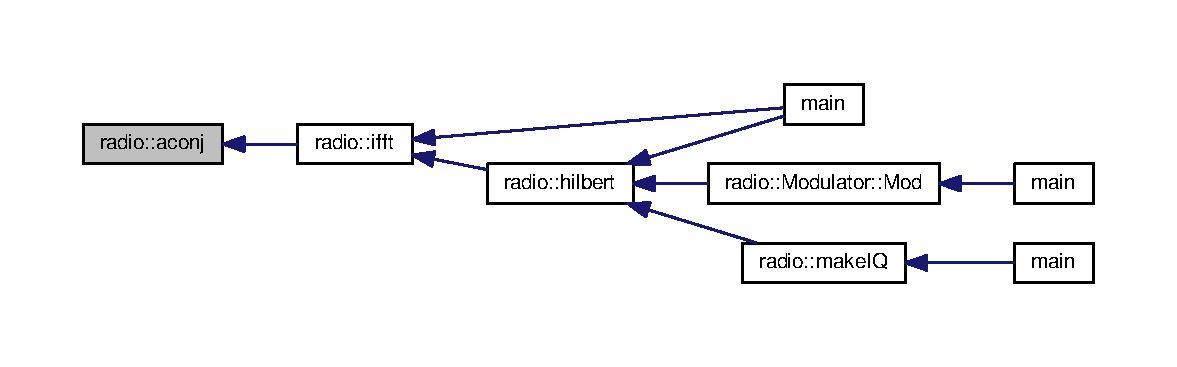
\includegraphics[width=350pt]{namespaceradio_aa04bb922c40cafb00a5603f1fc6d9c26_icgraph}
\end{center}
\end{figure}


\hypertarget{namespaceradio_ab146b5bf7f1c005939b024c9c4910a77}{\index{radio@{radio}!fft@{fft}}
\index{fft@{fft}!radio@{radio}}
\subsubsection[{fft}]{\setlength{\rightskip}{0pt plus 5cm}void radio\+::fft (
\begin{DoxyParamCaption}
\item[{{\bf cfloat32} $\ast$}]{data, }
\item[{{\bf uint32}}]{size}
\end{DoxyParamCaption}
)}}\label{namespaceradio_ab146b5bf7f1c005939b024c9c4910a77}
Replaces the values of an array of cfloat32's with the array's D\+F\+T using a decimation-\/in-\/frequency algorithm.

This code is based on code from \href{http://rosettacode.org/wiki/Fast_Fourier_transform#C.2B.2B}{\tt http\+://rosettacode.\+org/wiki/\+Fast\+\_\+\+Fourier\+\_\+transform\#\+C.\+2\+B.\+2\+B}.


\begin{DoxyParams}{Parameters}
{\em data} & the array whose values should be replaced with its D\+F\+T\\
\hline
{\em size} & the number of elements in the data array \\
\hline
\end{DoxyParams}


Definition at line 90 of file zdomain.\+hpp.



Here is the caller graph for this function\+:
\nopagebreak
\begin{figure}[H]
\begin{center}
\leavevmode
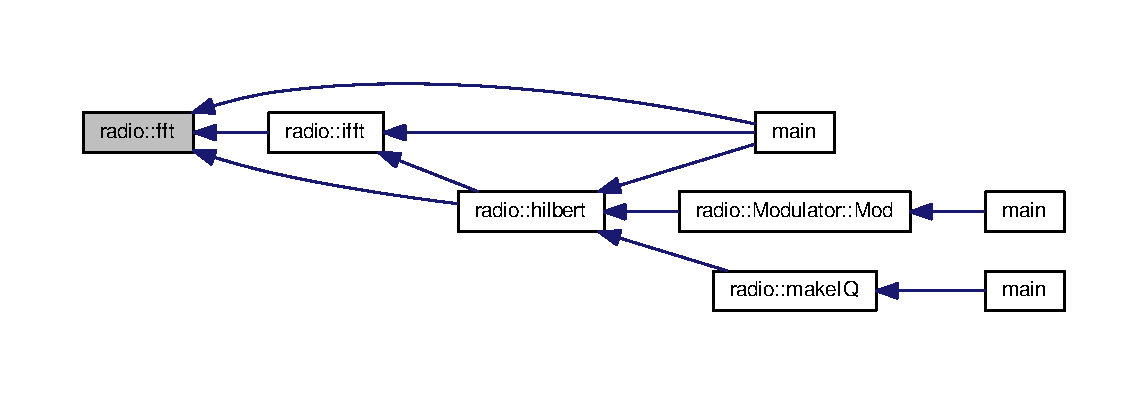
\includegraphics[width=350pt]{namespaceradio_ab146b5bf7f1c005939b024c9c4910a77_icgraph}
\end{center}
\end{figure}


\hypertarget{namespaceradio_a285a47b4ed81e5662d2b6b4bae0188d0}{\index{radio@{radio}!hilbert@{hilbert}}
\index{hilbert@{hilbert}!radio@{radio}}
\subsubsection[{hilbert}]{\setlength{\rightskip}{0pt plus 5cm}void radio\+::hilbert (
\begin{DoxyParamCaption}
\item[{{\bf float32} $\ast$}]{data, }
\item[{{\bf float32} $\ast$}]{dest, }
\item[{{\bf uint32}}]{size}
\end{DoxyParamCaption}
)}}\label{namespaceradio_a285a47b4ed81e5662d2b6b4bae0188d0}
Performs the hilbert transfor of an array of float32's.


\begin{DoxyParams}{Parameters}
{\em data} & the source array of the R\+E\+A\+L numbers of which to take the Hilbert transform\\
\hline
{\em dest} & the destination array of R\+E\+A\+L numbers for the results of the Hilbert transform\\
\hline
{\em size} & the number of elements in the data and dest arrays \\
\hline
\end{DoxyParams}


Definition at line 138 of file zdomain.\+hpp.



Here is the call graph for this function\+:
\nopagebreak
\begin{figure}[H]
\begin{center}
\leavevmode
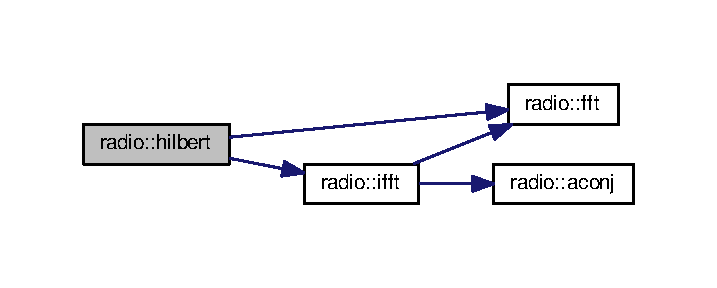
\includegraphics[width=344pt]{namespaceradio_a285a47b4ed81e5662d2b6b4bae0188d0_cgraph}
\end{center}
\end{figure}




Here is the caller graph for this function\+:
\nopagebreak
\begin{figure}[H]
\begin{center}
\leavevmode
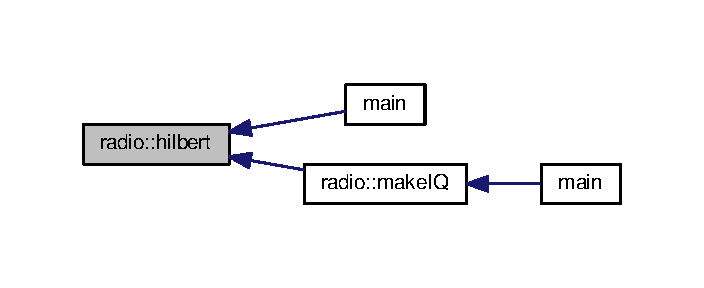
\includegraphics[width=350pt]{namespaceradio_a285a47b4ed81e5662d2b6b4bae0188d0_icgraph}
\end{center}
\end{figure}


\hypertarget{namespaceradio_a51add4e2faf6d58cabc3b4a3892420eb}{\index{radio@{radio}!ifft@{ifft}}
\index{ifft@{ifft}!radio@{radio}}
\subsubsection[{ifft}]{\setlength{\rightskip}{0pt plus 5cm}void radio\+::ifft (
\begin{DoxyParamCaption}
\item[{{\bf cfloat32} $\ast$}]{data, }
\item[{{\bf uint32}}]{size}
\end{DoxyParamCaption}
)}}\label{namespaceradio_a51add4e2faf6d58cabc3b4a3892420eb}
Replaces the values of an array of cfloat32's with the array's inverse D\+F\+T.

This code is based on code from \href{http://rosettacode.org/wiki/Fast_Fourier_transform#C.2B.2B}{\tt http\+://rosettacode.\+org/wiki/\+Fast\+\_\+\+Fourier\+\_\+transform\#\+C.\+2\+B.\+2\+B}.


\begin{DoxyParams}{Parameters}
{\em data} & the array whose values should be replaced with its inverse D\+F\+T\\
\hline
{\em size} & the number of elements in the data array \\
\hline
\end{DoxyParams}


Definition at line 158 of file zdomain.\+hpp.



Here is the call graph for this function\+:
\nopagebreak
\begin{figure}[H]
\begin{center}
\leavevmode
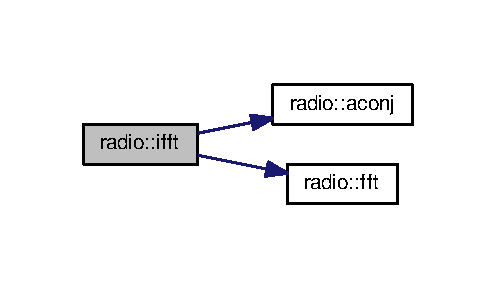
\includegraphics[width=238pt]{namespaceradio_a51add4e2faf6d58cabc3b4a3892420eb_cgraph}
\end{center}
\end{figure}




Here is the caller graph for this function\+:
\nopagebreak
\begin{figure}[H]
\begin{center}
\leavevmode
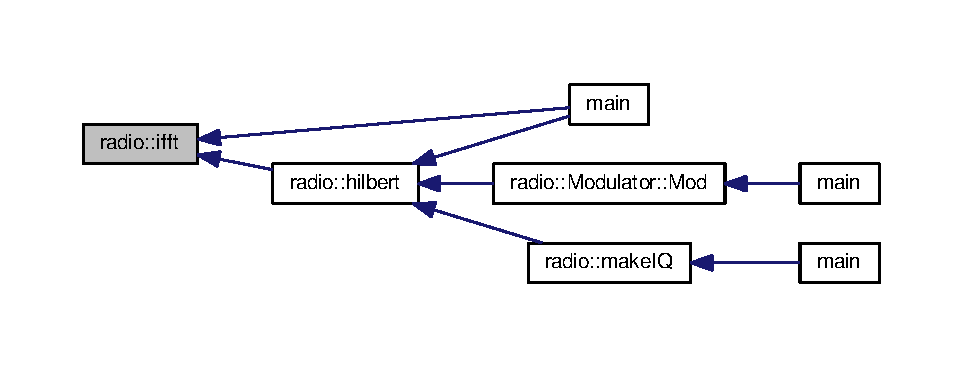
\includegraphics[width=350pt]{namespaceradio_a51add4e2faf6d58cabc3b4a3892420eb_icgraph}
\end{center}
\end{figure}


\hypertarget{namespaceradio_a7166522e76ff88e8d482491b1b6e2275}{\index{radio@{radio}!make\+I\+Q@{make\+I\+Q}}
\index{make\+I\+Q@{make\+I\+Q}!radio@{radio}}
\subsubsection[{make\+I\+Q}]{\setlength{\rightskip}{0pt plus 5cm}void radio\+::make\+I\+Q (
\begin{DoxyParamCaption}
\item[{{\bf float32} $\ast$}]{data, }
\item[{{\bf float32} $\ast$}]{dest, }
\item[{{\bf uint32}}]{size}
\end{DoxyParamCaption}
)}}\label{namespaceradio_a7166522e76ff88e8d482491b1b6e2275}
Produces an interleaved array of first an element from an original array of data and then an element from the original data's Hilbert transform. This function is intended to generate a two-\/channel output (I/\+Q output) for mixing applications.


\begin{DoxyParams}{Parameters}
{\em data} & the original data (left channel)\\
\hline
{\em dest} & the interleaved data (left channel original data, right channel transformed data) twice the size of the original data array\\
\hline
{\em size} & the number of elements in the data array (N\+O\+T in the destination array) \\
\hline
\end{DoxyParams}


Definition at line 168 of file zdomain.\+hpp.



Here is the call graph for this function\+:
\nopagebreak
\begin{figure}[H]
\begin{center}
\leavevmode
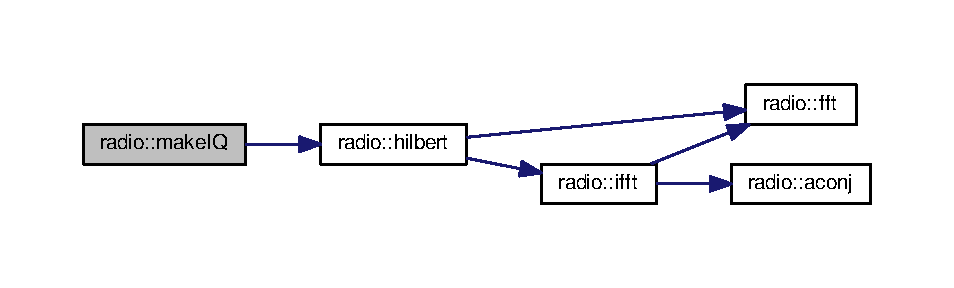
\includegraphics[width=350pt]{namespaceradio_a7166522e76ff88e8d482491b1b6e2275_cgraph}
\end{center}
\end{figure}




Here is the caller graph for this function\+:
\nopagebreak
\begin{figure}[H]
\begin{center}
\leavevmode
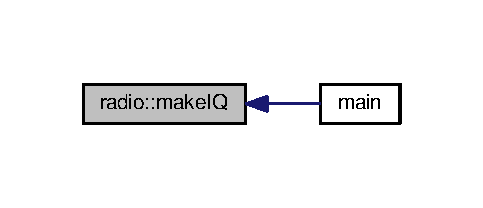
\includegraphics[width=232pt]{namespaceradio_a7166522e76ff88e8d482491b1b6e2275_icgraph}
\end{center}
\end{figure}


\hypertarget{namespaceradio_a6db7c682d0f9aeac8cb5042717b8ae7f}{\index{radio@{radio}!Show\+Help@{Show\+Help}}
\index{Show\+Help@{Show\+Help}!radio@{radio}}
\subsubsection[{Show\+Help}]{\setlength{\rightskip}{0pt plus 5cm}void radio\+::\+Show\+Help (
\begin{DoxyParamCaption}
{}
\end{DoxyParamCaption}
)}}\label{namespaceradio_a6db7c682d0f9aeac8cb5042717b8ae7f}
Displays the help information. 

Definition at line 20 of file auxiliary.\+hpp.



Here is the caller graph for this function\+:
\nopagebreak
\begin{figure}[H]
\begin{center}
\leavevmode
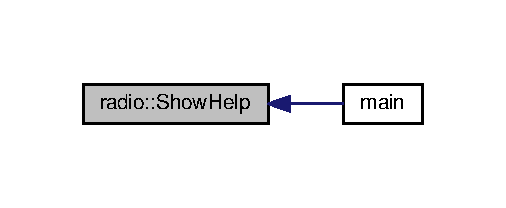
\includegraphics[width=243pt]{namespaceradio_a6db7c682d0f9aeac8cb5042717b8ae7f_icgraph}
\end{center}
\end{figure}


\hypertarget{namespaceradio_a402fe28e2e2bb2be7a0d2d9f74cc640d}{\index{radio@{radio}!to\+\_\+type@{to\+\_\+type}}
\index{to\+\_\+type@{to\+\_\+type}!radio@{radio}}
\subsubsection[{to\+\_\+type}]{\setlength{\rightskip}{0pt plus 5cm}{\bf Modulation\+Type} radio\+::to\+\_\+type (
\begin{DoxyParamCaption}
\item[{std\+::string}]{str}
\end{DoxyParamCaption}
)}}\label{namespaceradio_a402fe28e2e2bb2be7a0d2d9f74cc640d}
Converts a string representation of the supported modulation types (see \hyperlink{namespaceradio_a6db7c682d0f9aeac8cb5042717b8ae7f}{Show\+Help()} documentation) to the enum Modulation\+Type value.

This function is not as elegant as it could be. Ideally, I would have used a std\+::map$<$string, Modulation\+Type$>$ rather than a long series of if-\/else's.


\begin{DoxyParams}{Parameters}
{\em str} & type of modulation in typed form\\
\hline
\end{DoxyParams}
\begin{DoxyReturn}{Returns}
enum value of the type of modulation 
\end{DoxyReturn}


Definition at line 58 of file auxiliary.\+hpp.



Here is the caller graph for this function\+:
\nopagebreak
\begin{figure}[H]
\begin{center}
\leavevmode
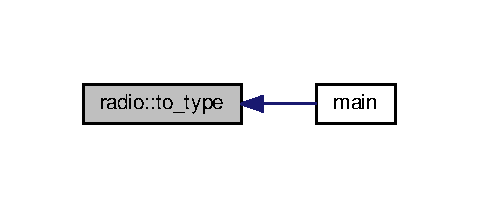
\includegraphics[width=230pt]{namespaceradio_a402fe28e2e2bb2be7a0d2d9f74cc640d_icgraph}
\end{center}
\end{figure}




\subsection{Variable Documentation}
\hypertarget{namespaceradio_a9bd902e9216499953a5906de73dc1796}{\index{radio@{radio}!F\+\_\+\+B\+A\+S\+E\+B\+A\+N\+D@{F\+\_\+\+B\+A\+S\+E\+B\+A\+N\+D}}
\index{F\+\_\+\+B\+A\+S\+E\+B\+A\+N\+D@{F\+\_\+\+B\+A\+S\+E\+B\+A\+N\+D}!radio@{radio}}
\subsubsection[{F\+\_\+\+B\+A\+S\+E\+B\+A\+N\+D}]{\setlength{\rightskip}{0pt plus 5cm}{\bf fparams} radio\+::\+F\+\_\+\+B\+A\+S\+E\+B\+A\+N\+D}}\label{namespaceradio_a9bd902e9216499953a5906de73dc1796}
{\bfseries Initial value\+:}
\begin{DoxyCode}
= \{ std::vector<float32> \{
        0.0008977019461,
            -0.002215694636,
            0.001372192986,
            0.001372192986,
            -0.002215694636,
            0.0008977019461 
    \}, std::vector<float32> \{
        1,
            -4.678616047,
            8.822912216,
            -8.379911423,
            4.007629871,
            -0.7719064355
    \} \}
\end{DoxyCode}
Baseband filter coefficients. Generated with M\+A\+T\+L\+A\+B 2015\+A. 

Definition at line 19 of file fvectors.\+hpp.

\hypertarget{namespaceradio_a0ffd57d5a11ff70a1f55dbdc8ebe098d}{\index{radio@{radio}!F\+\_\+\+L\+O\+W\+E\+R\+S\+I\+D\+E\+B\+A\+N\+D@{F\+\_\+\+L\+O\+W\+E\+R\+S\+I\+D\+E\+B\+A\+N\+D}}
\index{F\+\_\+\+L\+O\+W\+E\+R\+S\+I\+D\+E\+B\+A\+N\+D@{F\+\_\+\+L\+O\+W\+E\+R\+S\+I\+D\+E\+B\+A\+N\+D}!radio@{radio}}
\subsubsection[{F\+\_\+\+L\+O\+W\+E\+R\+S\+I\+D\+E\+B\+A\+N\+D}]{\setlength{\rightskip}{0pt plus 5cm}{\bf fparams} radio\+::\+F\+\_\+\+L\+O\+W\+E\+R\+S\+I\+D\+E\+B\+A\+N\+D}}\label{namespaceradio_a0ffd57d5a11ff70a1f55dbdc8ebe098d}
{\bfseries Initial value\+:}
\begin{DoxyCode}
= \{ std::vector<float32> \{
        0.2758038938,
            2.763578892,
            12.83915043,
            36.47584915,
            70.37084961,
            96.76893616,
            96.76893616,
            70.37084961,
            36.47584915,
            12.83915043,
            2.763578892,
            0.2758038938
    \}, std::vector<float32> \{
        1,
            7.605497837,
            27.34180641,
            60.83375549,
            92.60908508,
            100.8363876,
            79.74796295,
            45.49822617,
            18.1356678,
            4.690036297,
            0.6617552638,
            0.0281427335      
    \} \}
\end{DoxyCode}
Lower-\/sideband filter coefficients. Generated with M\+A\+T\+L\+A\+B 2015\+A. 

Definition at line 38 of file fvectors.\+hpp.

\hypertarget{namespaceradio_a0ec4548711b6d6ed6867c70b3fc2a413}{\index{radio@{radio}!F\+\_\+\+U\+P\+P\+E\+R\+S\+I\+D\+E\+B\+A\+N\+D@{F\+\_\+\+U\+P\+P\+E\+R\+S\+I\+D\+E\+B\+A\+N\+D}}
\index{F\+\_\+\+U\+P\+P\+E\+R\+S\+I\+D\+E\+B\+A\+N\+D@{F\+\_\+\+U\+P\+P\+E\+R\+S\+I\+D\+E\+B\+A\+N\+D}!radio@{radio}}
\subsubsection[{F\+\_\+\+U\+P\+P\+E\+R\+S\+I\+D\+E\+B\+A\+N\+D}]{\setlength{\rightskip}{0pt plus 5cm}{\bf fparams} radio\+::\+F\+\_\+\+U\+P\+P\+E\+R\+S\+I\+D\+E\+B\+A\+N\+D}}\label{namespaceradio_a0ec4548711b6d6ed6867c70b3fc2a413}
{\bfseries Initial value\+:}
\begin{DoxyCode}
= \{ std::vector<float32> \{
        0.001690387726,
            0.01145271584,
            0.03591799363,
            0.06576926261,
            0.0711934343,
            0.03156377375,
            -0.03156377375,
            -0.0711934343,
            -0.06576926261,
            -0.03591799363,
            -0.01145271584,
            -0.001690387726
    \}, std::vector<float32> \{
        1,
            9.465174675,
            41.62402725,
            112.0970993,
            205.2097626,
            267.9378662,
            254.4868011,
            175.7772827,
            86.5161972,
            28.89988136,
            5.897814751,
            0.5572910309
    \} \}
\end{DoxyCode}
Upper-\/sideband filter coefficients. Generated with M\+A\+T\+L\+A\+B 2015\+A. 

Definition at line 69 of file fvectors.\+hpp.

\hypertarget{namespaceradio_aa82ddc6ba206798fd70ffc25665b3cb6}{\index{radio@{radio}!F\+R\+E\+Q\+\_\+\+I\+N\+T\+E\+R\+M\+E\+D\+I\+A\+T\+E@{F\+R\+E\+Q\+\_\+\+I\+N\+T\+E\+R\+M\+E\+D\+I\+A\+T\+E}}
\index{F\+R\+E\+Q\+\_\+\+I\+N\+T\+E\+R\+M\+E\+D\+I\+A\+T\+E@{F\+R\+E\+Q\+\_\+\+I\+N\+T\+E\+R\+M\+E\+D\+I\+A\+T\+E}!radio@{radio}}
\subsubsection[{F\+R\+E\+Q\+\_\+\+I\+N\+T\+E\+R\+M\+E\+D\+I\+A\+T\+E}]{\setlength{\rightskip}{0pt plus 5cm}const {\bf uint32} radio\+::\+F\+R\+E\+Q\+\_\+\+I\+N\+T\+E\+R\+M\+E\+D\+I\+A\+T\+E = 20000}}\label{namespaceradio_aa82ddc6ba206798fd70ffc25665b3cb6}
The default intermediate carrier frequency 

Definition at line 26 of file Modulator.\+hpp.

\hypertarget{namespaceradio_a284213fea4beed2f74bb936927cbe654}{\index{radio@{radio}!S\+A\+M\+P\+L\+I\+N\+G\+\_\+\+R\+A\+T\+E@{S\+A\+M\+P\+L\+I\+N\+G\+\_\+\+R\+A\+T\+E}}
\index{S\+A\+M\+P\+L\+I\+N\+G\+\_\+\+R\+A\+T\+E@{S\+A\+M\+P\+L\+I\+N\+G\+\_\+\+R\+A\+T\+E}!radio@{radio}}
\subsubsection[{S\+A\+M\+P\+L\+I\+N\+G\+\_\+\+R\+A\+T\+E}]{\setlength{\rightskip}{0pt plus 5cm}const {\bf uint32} radio\+::\+S\+A\+M\+P\+L\+I\+N\+G\+\_\+\+R\+A\+T\+E = 48000}}\label{namespaceradio_a284213fea4beed2f74bb936927cbe654}
The default sampling rate (frequency) 

Definition at line 31 of file Modulator.\+hpp.


\chapter{Class Documentation}
\hypertarget{classradio_1_1Filter}{\section{radio\+:\+:Filter Class Reference}
\label{classradio_1_1Filter}\index{radio\+::\+Filter@{radio\+::\+Filter}}
}


{\ttfamily \#include $<$Filter.\+hpp$>$}

\subsection*{Public Member Functions}
\begin{DoxyCompactItemize}
\item 
\hyperlink{classradio_1_1Filter_a48ab268192e0135e5c9f74ad35a90fa1}{Filter} (\hyperlink{definitions_8hpp_aacdc525d6f7bddb3ae95d5c311bd06a1}{float32} $\ast$\hyperlink{classradio_1_1Filter_a25459a2b762120df0102f00553344be2}{data}, \hyperlink{definitions_8hpp_a1134b580f8da4de94ca6b1de4d37975e}{uint32} \hyperlink{classradio_1_1Filter_a7285b4c7263d8278e38abb14b5dca5d9}{size}, \hyperlink{definitions_8hpp_af19387f95516e2132a08cf60503f22a5}{fparams} \&\hyperlink{classradio_1_1Filter_abe705768a267844edfa2aaabfdac9f56}{diff\+Eq})
\item 
void \hyperlink{classradio_1_1Filter_ad2793821801780809af385463bf8f197}{Pass} ()
\end{DoxyCompactItemize}
\subsection*{Protected Attributes}
\begin{DoxyCompactItemize}
\item 
\hyperlink{definitions_8hpp_adde6aaee8457bee49c2a92621fe22b79}{uint8} \hyperlink{classradio_1_1Filter_a26a32320c4dffa8925ab5f0f06689e8d}{eq\+Length}
\item 
\hyperlink{definitions_8hpp_a1134b580f8da4de94ca6b1de4d37975e}{uint32} \hyperlink{classradio_1_1Filter_a7285b4c7263d8278e38abb14b5dca5d9}{size}
\item 
\hyperlink{definitions_8hpp_aacdc525d6f7bddb3ae95d5c311bd06a1}{float32} $\ast$ \hyperlink{classradio_1_1Filter_a25459a2b762120df0102f00553344be2}{data}
\item 
\hyperlink{definitions_8hpp_af19387f95516e2132a08cf60503f22a5}{fparams} \hyperlink{classradio_1_1Filter_abe705768a267844edfa2aaabfdac9f56}{diff\+Eq}
\item 
\hyperlink{definitions_8hpp_af19387f95516e2132a08cf60503f22a5}{fparams} \hyperlink{classradio_1_1Filter_ae7e324e76354063772bcb5f241a2eae9}{prev}
\end{DoxyCompactItemize}


\subsection{Detailed Description}
This class implements a z-\/domain filter on a specified array of float32'''s (a.\+k.\+a. singles, floats). It requires the transfer function coefficients already be calculated (i.\+e., it does not generate the coefficients based on desired filter characteristics). M\+A\+T\+L\+A\+B and its Signal Processing Toolbox can be used to generate the coefficients.

While this class is designed to implement a single-\/section filter, several instances of the class can be created and run over the data array sequentially to effectively implement a multi-\/section filter.

The class is designed (but not tested!) to allow for a z-\/domain transfer function with different orders of the zeros (numerator) and poles (denominator). 

Definition at line 31 of file Filter.\+hpp.



\subsection{Constructor \& Destructor Documentation}
\hypertarget{classradio_1_1Filter_a48ab268192e0135e5c9f74ad35a90fa1}{\index{radio\+::\+Filter@{radio\+::\+Filter}!Filter@{Filter}}
\index{Filter@{Filter}!radio\+::\+Filter@{radio\+::\+Filter}}
\subsubsection[{Filter}]{\setlength{\rightskip}{0pt plus 5cm}radio\+::\+Filter\+::\+Filter (
\begin{DoxyParamCaption}
\item[{{\bf float32} $\ast$}]{data, }
\item[{{\bf uint32}}]{size, }
\item[{{\bf fparams} \&}]{diff\+Eq}
\end{DoxyParamCaption}
)}}\label{classradio_1_1Filter_a48ab268192e0135e5c9f74ad35a90fa1}
Initializes \hyperlink{classradio_1_1Filter}{Filter} based on a difference equation.


\begin{DoxyParams}{Parameters}
{\em data} & array to be filtered. The filtered data will be placed here.\\
\hline
{\em size} & number of elements in the data array\\
\hline
{\em diff\+Eq} & a vector containing two vectors of float32'''s (a.\+k.\+a. singles, floats), containing the numerator and denominator coefficients, respectively, of the z-\/domain tranfer function of the filter in decending order (z$^\wedge$0, z$^\wedge$-\/1, z$^\wedge$-\/2, etc.). \\
\hline
\end{DoxyParams}


Definition at line 91 of file Filter.\+hpp.



\subsection{Member Function Documentation}
\hypertarget{classradio_1_1Filter_ad2793821801780809af385463bf8f197}{\index{radio\+::\+Filter@{radio\+::\+Filter}!Pass@{Pass}}
\index{Pass@{Pass}!radio\+::\+Filter@{radio\+::\+Filter}}
\subsubsection[{Pass}]{\setlength{\rightskip}{0pt plus 5cm}void radio\+::\+Filter\+::\+Pass (
\begin{DoxyParamCaption}
{}
\end{DoxyParamCaption}
)}}\label{classradio_1_1Filter_ad2793821801780809af385463bf8f197}
Passes the data array through the digital filter and accounts for x\mbox{[}n\mbox{]} and y\mbox{[}n\mbox{]} values from the previous call to \hyperlink{classradio_1_1Filter_ad2793821801780809af385463bf8f197}{Pass()}. 

Definition at line 111 of file Filter.\+hpp.



Here is the caller graph for this function\+:
\nopagebreak
\begin{figure}[H]
\begin{center}
\leavevmode
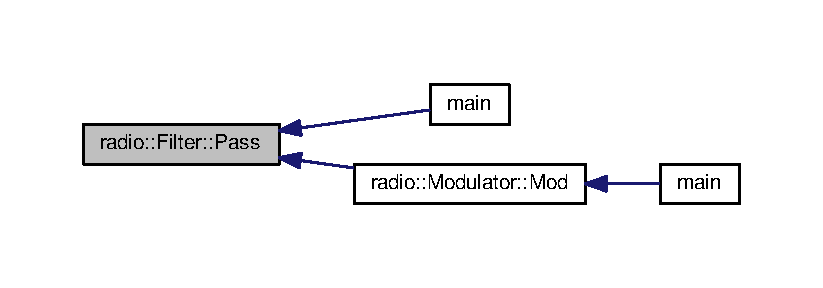
\includegraphics[width=248pt]{classradio_1_1Filter_ad2793821801780809af385463bf8f197_icgraph}
\end{center}
\end{figure}




\subsection{Member Data Documentation}
\hypertarget{classradio_1_1Filter_a25459a2b762120df0102f00553344be2}{\index{radio\+::\+Filter@{radio\+::\+Filter}!data@{data}}
\index{data@{data}!radio\+::\+Filter@{radio\+::\+Filter}}
\subsubsection[{data}]{\setlength{\rightskip}{0pt plus 5cm}{\bf float32}$\ast$ radio\+::\+Filter\+::data\hspace{0.3cm}{\ttfamily [protected]}}}\label{classradio_1_1Filter_a25459a2b762120df0102f00553344be2}
A pointer to the data array that should be filtered when \hyperlink{classradio_1_1Filter_ad2793821801780809af385463bf8f197}{Pass()} is called. 

Definition at line 71 of file Filter.\+hpp.

\hypertarget{classradio_1_1Filter_abe705768a267844edfa2aaabfdac9f56}{\index{radio\+::\+Filter@{radio\+::\+Filter}!diff\+Eq@{diff\+Eq}}
\index{diff\+Eq@{diff\+Eq}!radio\+::\+Filter@{radio\+::\+Filter}}
\subsubsection[{diff\+Eq}]{\setlength{\rightskip}{0pt plus 5cm}{\bf fparams} radio\+::\+Filter\+::diff\+Eq\hspace{0.3cm}{\ttfamily [protected]}}}\label{classradio_1_1Filter_abe705768a267844edfa2aaabfdac9f56}
A vector containing two vectors of float32'''s (a.\+k.\+a. singles, floats), containing the numerator and denominator coefficients, respectively, of the z-\/domain tranfer function of the filter in decending order (z$^\wedge$0, z$^\wedge$-\/1, z$^\wedge$-\/2, etc.). 

Definition at line 79 of file Filter.\+hpp.

\hypertarget{classradio_1_1Filter_a26a32320c4dffa8925ab5f0f06689e8d}{\index{radio\+::\+Filter@{radio\+::\+Filter}!eq\+Length@{eq\+Length}}
\index{eq\+Length@{eq\+Length}!radio\+::\+Filter@{radio\+::\+Filter}}
\subsubsection[{eq\+Length}]{\setlength{\rightskip}{0pt plus 5cm}{\bf uint8} radio\+::\+Filter\+::eq\+Length\hspace{0.3cm}{\ttfamily [protected]}}}\label{classradio_1_1Filter_a26a32320c4dffa8925ab5f0f06689e8d}
The order of the filter transfer function (i.\+e., the maximum of the orders of the numerator and denominator). 

Definition at line 60 of file Filter.\+hpp.

\hypertarget{classradio_1_1Filter_ae7e324e76354063772bcb5f241a2eae9}{\index{radio\+::\+Filter@{radio\+::\+Filter}!prev@{prev}}
\index{prev@{prev}!radio\+::\+Filter@{radio\+::\+Filter}}
\subsubsection[{prev}]{\setlength{\rightskip}{0pt plus 5cm}{\bf fparams} radio\+::\+Filter\+::prev\hspace{0.3cm}{\ttfamily [protected]}}}\label{classradio_1_1Filter_ae7e324e76354063772bcb5f241a2eae9}
Vectors of the original (x\mbox{[}n\mbox{]}) and filtered (y\mbox{[}n\mbox{]}) values of the data array used to calculate the first filtered values of the data array. In spite of the type name, this variable does N\+O\+T contains filter parameters but rather the same data type that fparams represents. 

Definition at line 88 of file Filter.\+hpp.

\hypertarget{classradio_1_1Filter_a7285b4c7263d8278e38abb14b5dca5d9}{\index{radio\+::\+Filter@{radio\+::\+Filter}!size@{size}}
\index{size@{size}!radio\+::\+Filter@{radio\+::\+Filter}}
\subsubsection[{size}]{\setlength{\rightskip}{0pt plus 5cm}{\bf uint32} radio\+::\+Filter\+::size\hspace{0.3cm}{\ttfamily [protected]}}}\label{classradio_1_1Filter_a7285b4c7263d8278e38abb14b5dca5d9}
The number of elements in the data array. 

Definition at line 65 of file Filter.\+hpp.



The documentation for this class was generated from the following file\+:\begin{DoxyCompactItemize}
\item 
src/\hyperlink{Filter_8hpp}{Filter.\+hpp}\end{DoxyCompactItemize}

\hypertarget{classradio_1_1Gain}{\section{radio\+:\+:Gain Class Reference}
\label{classradio_1_1Gain}\index{radio\+::\+Gain@{radio\+::\+Gain}}
}


{\ttfamily \#include $<$Gain.\+hpp$>$}

\subsection*{Public Member Functions}
\begin{DoxyCompactItemize}
\item 
\hyperlink{classradio_1_1Gain_a11f137515c0ecc04333c7d92eea2cf79}{Gain} (\hyperlink{definitions_8hpp_aacdc525d6f7bddb3ae95d5c311bd06a1}{float32} $\ast$data, \hyperlink{definitions_8hpp_a1134b580f8da4de94ca6b1de4d37975e}{uint32} size, \hyperlink{definitions_8hpp_aacdc525d6f7bddb3ae95d5c311bd06a1}{float32} gaind\+B)
\item 
void \hyperlink{classradio_1_1Gain_a8c6df2c5989da0e560c8f276e6138a2d}{Apply} ()
\end{DoxyCompactItemize}


\subsection{Detailed Description}
Applies a gain to a (baseband) signal. 

Definition at line \hyperlink{Gain_8hpp_source_l00018}{18} of file \hyperlink{Gain_8hpp_source}{Gain.\+hpp}.



\subsection{Constructor \& Destructor Documentation}
\hypertarget{classradio_1_1Gain_a11f137515c0ecc04333c7d92eea2cf79}{\index{radio\+::\+Gain@{radio\+::\+Gain}!Gain@{Gain}}
\index{Gain@{Gain}!radio\+::\+Gain@{radio\+::\+Gain}}
\subsubsection[{Gain}]{\setlength{\rightskip}{0pt plus 5cm}radio\+::\+Gain\+::\+Gain (
\begin{DoxyParamCaption}
\item[{{\bf float32} $\ast$}]{data, }
\item[{{\bf uint32}}]{size, }
\item[{{\bf float32}}]{gaind\+B}
\end{DoxyParamCaption}
)}}\label{classradio_1_1Gain_a11f137515c0ecc04333c7d92eea2cf79}
Initializes a \hyperlink{classradio_1_1Gain}{Gain} object and converts gain from decibels to a standard value.


\begin{DoxyParams}{Parameters}
{\em data} & the signal to which the gain is applied\\
\hline
{\em size} & the number of elements in the data array\\
\hline
{\em gaind\+B} & the desired gain in decibels (of power) \\
\hline
\end{DoxyParams}


Definition at line \hyperlink{Gain_8hpp_source_l00061}{61} of file \hyperlink{Gain_8hpp_source}{Gain.\+hpp}.


\begin{DoxyCode}
00061                                                          \{
00062         this->data = data;
00063         this->size = size;
00064         gainCoeff = pow(10, gaindB / 20);
00065     \}
\end{DoxyCode}


\subsection{Member Function Documentation}
\hypertarget{classradio_1_1Gain_a8c6df2c5989da0e560c8f276e6138a2d}{\index{radio\+::\+Gain@{radio\+::\+Gain}!Apply@{Apply}}
\index{Apply@{Apply}!radio\+::\+Gain@{radio\+::\+Gain}}
\subsubsection[{Apply}]{\setlength{\rightskip}{0pt plus 5cm}void radio\+::\+Gain\+::\+Apply (
\begin{DoxyParamCaption}
{}
\end{DoxyParamCaption}
)}}\label{classradio_1_1Gain_a8c6df2c5989da0e560c8f276e6138a2d}
Applies the gain to the signal contained in the data array 

Definition at line \hyperlink{Gain_8hpp_source_l00067}{67} of file \hyperlink{Gain_8hpp_source}{Gain.\+hpp}.


\begin{DoxyCode}
00067                      \{
00068         \textcolor{keywordflow}{for}(\hyperlink{definitions_8hpp_a1134b580f8da4de94ca6b1de4d37975e}{uint32} i = 0; i < size; i++) \{
00069             data[i] *= gainCoeff;
00070 
00071             \textcolor{keywordflow}{if}((data[i] > 1 || data[i] < -1) && !hasClipped) \{
00072                 hasClipped = \textcolor{keyword}{true};
00073                 std::cerr << \textcolor{stringliteral}{"Baseband clipping has occurred!"}
00074                     << std::endl;
00075             \}
00076         \}
00077     \}
\end{DoxyCode}


Here is the caller graph for this function\+:
\nopagebreak
\begin{figure}[H]
\begin{center}
\leavevmode
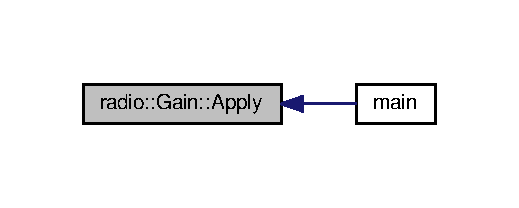
\includegraphics[width=249pt]{classradio_1_1Gain_a8c6df2c5989da0e560c8f276e6138a2d_icgraph}
\end{center}
\end{figure}




The documentation for this class was generated from the following file\+:\begin{DoxyCompactItemize}
\item 
src/\hyperlink{Gain_8hpp}{Gain.\+hpp}\end{DoxyCompactItemize}

\hypertarget{classradio_1_1Modulator}{\section{radio\+:\+:Modulator Class Reference}
\label{classradio_1_1Modulator}\index{radio\+::\+Modulator@{radio\+::\+Modulator}}
}


{\ttfamily \#include $<$modulation.\+hpp$>$}



Inheritance diagram for radio\+:\+:Modulator\+:
\nopagebreak
\begin{figure}[H]
\begin{center}
\leavevmode
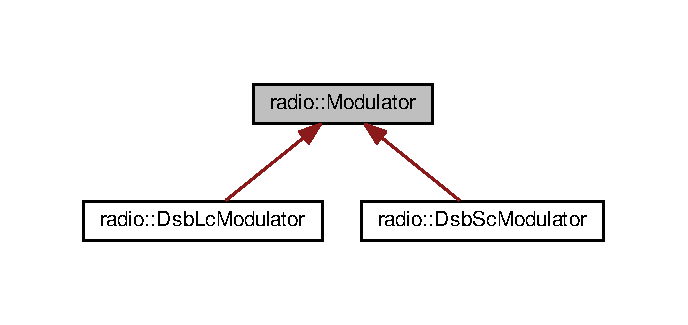
\includegraphics[width=330pt]{classradio_1_1Modulator__inherit__graph}
\end{center}
\end{figure}
\subsection*{Public Member Functions}
\begin{DoxyCompactItemize}
\item 
virtual void \hyperlink{classradio_1_1Modulator_a44e9de3acd9499b31da5064b039e7a15}{Mod} ()=0
\end{DoxyCompactItemize}
\subsection*{Protected Member Functions}
\begin{DoxyCompactItemize}
\item 
\hyperlink{classradio_1_1Modulator_a4ce73238d07f8703b7b905c9c6dba28e}{Modulator} (\hyperlink{definitions_8hpp_aacdc525d6f7bddb3ae95d5c311bd06a1}{float32} \hyperlink{classradio_1_1Modulator_a39d698f7720aa3677ecaf1baf83c8fa0}{data}\mbox{[}$\,$\mbox{]}, \hyperlink{definitions_8hpp_a1134b580f8da4de94ca6b1de4d37975e}{uint32} \hyperlink{classradio_1_1Modulator_ad1fbba4bdd6a8c8d2ff05cb7be60fc5c}{size})
\item 
\hyperlink{classradio_1_1Modulator_a07ffbd7e75e18027c60e77d4fc5b5e37}{Modulator} (\hyperlink{definitions_8hpp_aacdc525d6f7bddb3ae95d5c311bd06a1}{float32} freq\+Inter, \hyperlink{definitions_8hpp_a1134b580f8da4de94ca6b1de4d37975e}{uint32} \hyperlink{classradio_1_1Modulator_a8901a2170e850a767dd40f9494dd7536}{rate}, \hyperlink{definitions_8hpp_aacdc525d6f7bddb3ae95d5c311bd06a1}{float32} \hyperlink{classradio_1_1Modulator_a39d698f7720aa3677ecaf1baf83c8fa0}{data}\mbox{[}$\,$\mbox{]}, \hyperlink{definitions_8hpp_a1134b580f8da4de94ca6b1de4d37975e}{uint32} \hyperlink{classradio_1_1Modulator_ad1fbba4bdd6a8c8d2ff05cb7be60fc5c}{size})
\end{DoxyCompactItemize}
\subsection*{Protected Attributes}
\begin{DoxyCompactItemize}
\item 
\hyperlink{definitions_8hpp_aacdc525d6f7bddb3ae95d5c311bd06a1}{float32} $\ast$ \hyperlink{classradio_1_1Modulator_a42d68c4f2d9819ede178b9dea23fecee}{carrier}
\item 
\hyperlink{definitions_8hpp_a1134b580f8da4de94ca6b1de4d37975e}{uint32} \hyperlink{classradio_1_1Modulator_a9a4b25f4589e30915ef4836c8b01cd93}{carr\+Ind} = 0
\item 
\hyperlink{definitions_8hpp_aacdc525d6f7bddb3ae95d5c311bd06a1}{float32} $\ast$ \hyperlink{classradio_1_1Modulator_a39d698f7720aa3677ecaf1baf83c8fa0}{data}
\item 
\hyperlink{definitions_8hpp_aacdc525d6f7bddb3ae95d5c311bd06a1}{float32} \hyperlink{classradio_1_1Modulator_a8901a2170e850a767dd40f9494dd7536}{rate}
\item 
\hyperlink{definitions_8hpp_a1134b580f8da4de94ca6b1de4d37975e}{uint32} \hyperlink{classradio_1_1Modulator_ad1fbba4bdd6a8c8d2ff05cb7be60fc5c}{size}
\end{DoxyCompactItemize}


\subsection{Detailed Description}
This class, while not intended to be called directly, is a superclass for the classes of the modulation forms used in this project. 

Definition at line 24 of file modulation.\+hpp.



\subsection{Constructor \& Destructor Documentation}
\hypertarget{classradio_1_1Modulator_a4ce73238d07f8703b7b905c9c6dba28e}{\index{radio\+::\+Modulator@{radio\+::\+Modulator}!Modulator@{Modulator}}
\index{Modulator@{Modulator}!radio\+::\+Modulator@{radio\+::\+Modulator}}
\subsubsection[{Modulator}]{\setlength{\rightskip}{0pt plus 5cm}radio\+::\+Modulator\+::\+Modulator (
\begin{DoxyParamCaption}
\item[{{\bf float32}}]{data\mbox{[}$\,$\mbox{]}, }
\item[{{\bf uint32}}]{size}
\end{DoxyParamCaption}
)\hspace{0.3cm}{\ttfamily [inline]}, {\ttfamily [protected]}}}\label{classradio_1_1Modulator_a4ce73238d07f8703b7b905c9c6dba28e}
Creates a \hyperlink{classradio_1_1Modulator}{Modulator} with a default carrier intermediate frequency and default sampling rate. Intended to be called only by subclasses.


\begin{DoxyParams}{Parameters}
{\em data} & the data array initially containing the baseband signal\\
\hline
{\em size} & the number of elements in the data array \\
\hline
\end{DoxyParams}


Definition at line 69 of file modulation.\+hpp.

\hypertarget{classradio_1_1Modulator_a07ffbd7e75e18027c60e77d4fc5b5e37}{\index{radio\+::\+Modulator@{radio\+::\+Modulator}!Modulator@{Modulator}}
\index{Modulator@{Modulator}!radio\+::\+Modulator@{radio\+::\+Modulator}}
\subsubsection[{Modulator}]{\setlength{\rightskip}{0pt plus 5cm}radio\+::\+Modulator\+::\+Modulator (
\begin{DoxyParamCaption}
\item[{{\bf float32}}]{freq\+Inter, }
\item[{{\bf uint32}}]{rate, }
\item[{{\bf float32}}]{data\mbox{[}$\,$\mbox{]}, }
\item[{{\bf uint32}}]{size}
\end{DoxyParamCaption}
)\hspace{0.3cm}{\ttfamily [protected]}}}\label{classradio_1_1Modulator_a07ffbd7e75e18027c60e77d4fc5b5e37}
Creates a \hyperlink{classradio_1_1Modulator}{Modulator} with the specified parameters. Intended to be called only by subclasses.


\begin{DoxyParams}{Parameters}
{\em freq\+Inter} & the frequency of the I\+F carrier sinusoid\\
\hline
{\em rate} & the sampling rate of the baseband and I\+F signals\\
\hline
{\em data} & the array holding initially the baseband signal\\
\hline
{\em size} & the number of elements in data \\
\hline
\end{DoxyParams}


Definition at line 176 of file modulation.\+hpp.



\subsection{Member Function Documentation}
\hypertarget{classradio_1_1Modulator_a44e9de3acd9499b31da5064b039e7a15}{\index{radio\+::\+Modulator@{radio\+::\+Modulator}!Mod@{Mod}}
\index{Mod@{Mod}!radio\+::\+Modulator@{radio\+::\+Modulator}}
\subsubsection[{Mod}]{\setlength{\rightskip}{0pt plus 5cm}virtual void radio\+::\+Modulator\+::\+Mod (
\begin{DoxyParamCaption}
{}
\end{DoxyParamCaption}
)\hspace{0.3cm}{\ttfamily [pure virtual]}}}\label{classradio_1_1Modulator_a44e9de3acd9499b31da5064b039e7a15}
Requires subclasses to implement a \hyperlink{classradio_1_1Modulator_a44e9de3acd9499b31da5064b039e7a15}{Mod()} function. 

Implemented in \hyperlink{classradio_1_1DsbScModulator_a0925dbd82745c282a488a45b0ee1410b}{radio\+::\+Dsb\+Sc\+Modulator}, and \hyperlink{classradio_1_1DsbLcModulator_ad6b7f8af29cadd93ffa104e598485c25}{radio\+::\+Dsb\+Lc\+Modulator}.



\subsection{Member Data Documentation}
\hypertarget{classradio_1_1Modulator_a42d68c4f2d9819ede178b9dea23fecee}{\index{radio\+::\+Modulator@{radio\+::\+Modulator}!carrier@{carrier}}
\index{carrier@{carrier}!radio\+::\+Modulator@{radio\+::\+Modulator}}
\subsubsection[{carrier}]{\setlength{\rightskip}{0pt plus 5cm}{\bf float32}$\ast$ radio\+::\+Modulator\+::carrier\hspace{0.3cm}{\ttfamily [protected]}}}\label{classradio_1_1Modulator_a42d68c4f2d9819ede178b9dea23fecee}
An array of sinusoid values of the carrier wave 

Definition at line 35 of file modulation.\+hpp.

\hypertarget{classradio_1_1Modulator_a9a4b25f4589e30915ef4836c8b01cd93}{\index{radio\+::\+Modulator@{radio\+::\+Modulator}!carr\+Ind@{carr\+Ind}}
\index{carr\+Ind@{carr\+Ind}!radio\+::\+Modulator@{radio\+::\+Modulator}}
\subsubsection[{carr\+Ind}]{\setlength{\rightskip}{0pt plus 5cm}{\bf uint32} radio\+::\+Modulator\+::carr\+Ind = 0\hspace{0.3cm}{\ttfamily [protected]}}}\label{classradio_1_1Modulator_a9a4b25f4589e30915ef4836c8b01cd93}
The index tracking the value of the carrier sinusoid (held in carrier) to be used in the next calculation 

Definition at line 41 of file modulation.\+hpp.

\hypertarget{classradio_1_1Modulator_a39d698f7720aa3677ecaf1baf83c8fa0}{\index{radio\+::\+Modulator@{radio\+::\+Modulator}!data@{data}}
\index{data@{data}!radio\+::\+Modulator@{radio\+::\+Modulator}}
\subsubsection[{data}]{\setlength{\rightskip}{0pt plus 5cm}{\bf float32}$\ast$ radio\+::\+Modulator\+::data\hspace{0.3cm}{\ttfamily [protected]}}}\label{classradio_1_1Modulator_a39d698f7720aa3677ecaf1baf83c8fa0}
The data to modulate (i.\+e., baseband signal), which is then replaced by its modulated signal of the same sampling rate 

Definition at line 47 of file modulation.\+hpp.

\hypertarget{classradio_1_1Modulator_a8901a2170e850a767dd40f9494dd7536}{\index{radio\+::\+Modulator@{radio\+::\+Modulator}!rate@{rate}}
\index{rate@{rate}!radio\+::\+Modulator@{radio\+::\+Modulator}}
\subsubsection[{rate}]{\setlength{\rightskip}{0pt plus 5cm}{\bf float32} radio\+::\+Modulator\+::rate\hspace{0.3cm}{\ttfamily [protected]}}}\label{classradio_1_1Modulator_a8901a2170e850a767dd40f9494dd7536}
The sampling rate of the baseband and generated I\+F signals 

Definition at line 52 of file modulation.\+hpp.

\hypertarget{classradio_1_1Modulator_ad1fbba4bdd6a8c8d2ff05cb7be60fc5c}{\index{radio\+::\+Modulator@{radio\+::\+Modulator}!size@{size}}
\index{size@{size}!radio\+::\+Modulator@{radio\+::\+Modulator}}
\subsubsection[{size}]{\setlength{\rightskip}{0pt plus 5cm}{\bf uint32} radio\+::\+Modulator\+::size\hspace{0.3cm}{\ttfamily [protected]}}}\label{classradio_1_1Modulator_ad1fbba4bdd6a8c8d2ff05cb7be60fc5c}
The number of elements in the data array 

Definition at line 57 of file modulation.\+hpp.



The documentation for this class was generated from the following file\+:\begin{DoxyCompactItemize}
\item 
src/\hyperlink{modulation_8hpp}{modulation.\+hpp}\end{DoxyCompactItemize}

\hypertarget{classradio_1_1PlTone}{\section{radio\+:\+:Pl\+Tone Class Reference}
\label{classradio_1_1PlTone}\index{radio\+::\+Pl\+Tone@{radio\+::\+Pl\+Tone}}
}


{\ttfamily \#include $<$Pl\+Tone.\+hpp$>$}



Inheritance diagram for radio\+:\+:Pl\+Tone\+:
\nopagebreak
\begin{figure}[H]
\begin{center}
\leavevmode
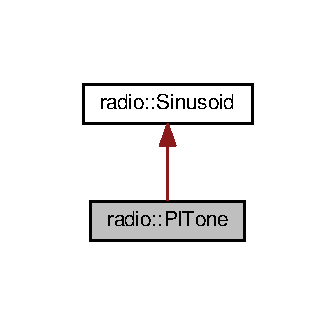
\includegraphics[width=161pt]{classradio_1_1PlTone__inherit__graph}
\end{center}
\end{figure}


Collaboration diagram for radio\+:\+:Pl\+Tone\+:
\nopagebreak
\begin{figure}[H]
\begin{center}
\leavevmode
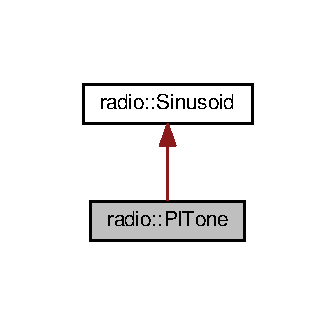
\includegraphics[width=161pt]{classradio_1_1PlTone__coll__graph}
\end{center}
\end{figure}
\subsection*{Public Member Functions}
\begin{DoxyCompactItemize}
\item 
\hyperlink{classradio_1_1PlTone_aaf1bc146478693f3e921bdc6f8ea2379}{Pl\+Tone} (\hyperlink{definitions_8hpp_aacdc525d6f7bddb3ae95d5c311bd06a1}{float32} amplitude, \hyperlink{definitions_8hpp_aacdc525d6f7bddb3ae95d5c311bd06a1}{float32} $\ast$data, \hyperlink{definitions_8hpp_a1134b580f8da4de94ca6b1de4d37975e}{uint32} size, \hyperlink{definitions_8hpp_aacdc525d6f7bddb3ae95d5c311bd06a1}{float32} \hyperlink{classradio_1_1Sinusoid_ad429b5dd330e96aaf89a0d48ef59d3f2}{frequency}, \hyperlink{definitions_8hpp_a1134b580f8da4de94ca6b1de4d37975e}{uint32} \hyperlink{classradio_1_1Sinusoid_a964d64aae9acc4ea5d752534a33d76b8}{sampling\+Rate})
\item 
void \hyperlink{classradio_1_1PlTone_a9e19b2d5106b35626d4839f04f9b9f95}{Add} ()
\end{DoxyCompactItemize}


\subsection{Detailed Description}
This class creates a C\+T\+C\+S\+S subcarrier (P\+L tone) at a specified frequency in a baseband signal. 

Definition at line \hyperlink{PlTone_8hpp_source_l00018}{18} of file \hyperlink{PlTone_8hpp_source}{Pl\+Tone.\+hpp}.



\subsection{Constructor \& Destructor Documentation}
\hypertarget{classradio_1_1PlTone_aaf1bc146478693f3e921bdc6f8ea2379}{\index{radio\+::\+Pl\+Tone@{radio\+::\+Pl\+Tone}!Pl\+Tone@{Pl\+Tone}}
\index{Pl\+Tone@{Pl\+Tone}!radio\+::\+Pl\+Tone@{radio\+::\+Pl\+Tone}}
\subsubsection[{Pl\+Tone}]{\setlength{\rightskip}{0pt plus 5cm}radio\+::\+Pl\+Tone\+::\+Pl\+Tone (
\begin{DoxyParamCaption}
\item[{{\bf float32}}]{amplitude, }
\item[{{\bf float32} $\ast$}]{data, }
\item[{{\bf uint32}}]{size, }
\item[{{\bf float32}}]{frequency, }
\item[{{\bf uint32}}]{sampling\+Rate}
\end{DoxyParamCaption}
)}}\label{classradio_1_1PlTone_aaf1bc146478693f3e921bdc6f8ea2379}
Creates a \hyperlink{classradio_1_1PlTone}{Pl\+Tone} object.


\begin{DoxyParams}{Parameters}
{\em amplitude} & the amplitude (0-\/1) of the subcarrier. Assumes baseband signal has a peak-\/to-\/peak range of -\/1 to 1.\\
\hline
{\em data} & an array containing a portion of the discrete baseband signal\\
\hline
{\em size} & the number of elemeents in the data array\\
\hline
{\em frequency} & the frequency of the C\+T\+C\+S\+S tone in the baseband (not in the I\+F or R\+F signals)\\
\hline
{\em sampling\+Rate} & the sampling frequency of the baseband signal \\
\hline
\end{DoxyParams}


Definition at line \hyperlink{PlTone_8hpp_source_l00063}{63} of file \hyperlink{PlTone_8hpp_source}{Pl\+Tone.\+hpp}.



\subsection{Member Function Documentation}
\hypertarget{classradio_1_1PlTone_a9e19b2d5106b35626d4839f04f9b9f95}{\index{radio\+::\+Pl\+Tone@{radio\+::\+Pl\+Tone}!Add@{Add}}
\index{Add@{Add}!radio\+::\+Pl\+Tone@{radio\+::\+Pl\+Tone}}
\subsubsection[{Add}]{\setlength{\rightskip}{0pt plus 5cm}void radio\+::\+Pl\+Tone\+::\+Add (
\begin{DoxyParamCaption}
{}
\end{DoxyParamCaption}
)}}\label{classradio_1_1PlTone_a9e19b2d5106b35626d4839f04f9b9f95}
Adds the C\+T\+C\+S\+S tone to the baseband signal. 

Definition at line \hyperlink{PlTone_8hpp_source_l00075}{75} of file \hyperlink{PlTone_8hpp_source}{Pl\+Tone.\+hpp}.



Here is the call graph for this function\+:
\nopagebreak
\begin{figure}[H]
\begin{center}
\leavevmode
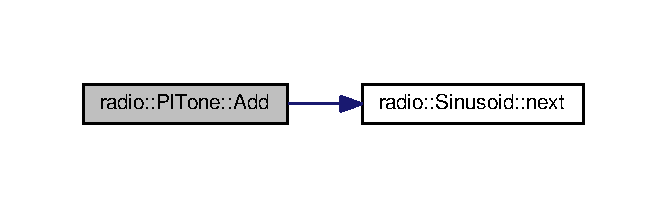
\includegraphics[width=320pt]{classradio_1_1PlTone_a9e19b2d5106b35626d4839f04f9b9f95_cgraph}
\end{center}
\end{figure}




Here is the caller graph for this function\+:
\nopagebreak
\begin{figure}[H]
\begin{center}
\leavevmode
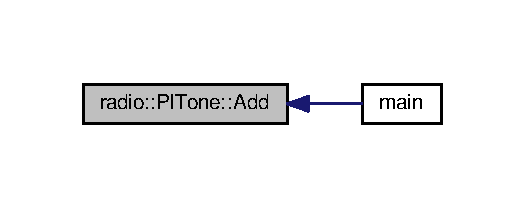
\includegraphics[width=252pt]{classradio_1_1PlTone_a9e19b2d5106b35626d4839f04f9b9f95_icgraph}
\end{center}
\end{figure}




The documentation for this class was generated from the following file\+:\begin{DoxyCompactItemize}
\item 
src/\hyperlink{PlTone_8hpp}{Pl\+Tone.\+hpp}\end{DoxyCompactItemize}

\hypertarget{classradio_1_1Sinusoid}{\section{radio\+:\+:Sinusoid Class Reference}
\label{classradio_1_1Sinusoid}\index{radio\+::\+Sinusoid@{radio\+::\+Sinusoid}}
}


{\ttfamily \#include $<$Sinusoid.\+hpp$>$}



Inheritance diagram for radio\+:\+:Sinusoid\+:
\nopagebreak
\begin{figure}[H]
\begin{center}
\leavevmode
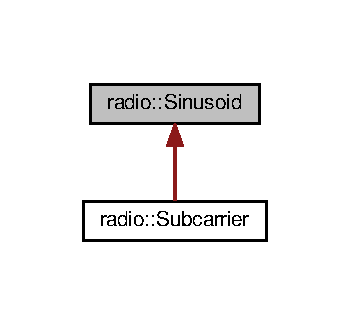
\includegraphics[width=161pt]{classradio_1_1Sinusoid__inherit__graph}
\end{center}
\end{figure}
\subsection*{Public Member Functions}
\begin{DoxyCompactItemize}
\item 
\hyperlink{classradio_1_1Sinusoid_a9494c3cb2bca12effdf770e10dfbe8a5}{Sinusoid} (\hyperlink{definitions_8hpp_aacdc525d6f7bddb3ae95d5c311bd06a1}{float32} \hyperlink{classradio_1_1Sinusoid_ad429b5dd330e96aaf89a0d48ef59d3f2}{frequency}, \hyperlink{definitions_8hpp_a1134b580f8da4de94ca6b1de4d37975e}{uint32} \hyperlink{classradio_1_1Sinusoid_a964d64aae9acc4ea5d752534a33d76b8}{sampling\+Rate}=48000)
\item 
\hyperlink{classradio_1_1Sinusoid_ad9e8edf233f8146891a14f20d1c903d2}{$\sim$\+Sinusoid} ()
\item 
\hyperlink{definitions_8hpp_aacdc525d6f7bddb3ae95d5c311bd06a1}{float32} \hyperlink{classradio_1_1Sinusoid_aab44298ea1bd5cb175d5826243cf56f2}{next} ()
\item 
\hyperlink{definitions_8hpp_aacdc525d6f7bddb3ae95d5c311bd06a1}{float32} \hyperlink{classradio_1_1Sinusoid_a3f2741e9dd30291e5fa87f2eb2243e7c}{next\+Shifted} ()
\end{DoxyCompactItemize}
\subsection*{Protected Attributes}
\begin{DoxyCompactItemize}
\item 
\hyperlink{definitions_8hpp_aacdc525d6f7bddb3ae95d5c311bd06a1}{float32} \hyperlink{classradio_1_1Sinusoid_ad429b5dd330e96aaf89a0d48ef59d3f2}{frequency}
\item 
\hyperlink{definitions_8hpp_a1134b580f8da4de94ca6b1de4d37975e}{uint32} \hyperlink{classradio_1_1Sinusoid_a2e7d029c5e7307967c77959367cc0224}{sin\+Index} = 0
\item 
\hyperlink{definitions_8hpp_a1134b580f8da4de94ca6b1de4d37975e}{uint32} \hyperlink{classradio_1_1Sinusoid_a4acf2add824249c39046fe87f9a64f93}{sin\+Index\+Shifted} = 0
\item 
\hyperlink{definitions_8hpp_a1134b580f8da4de94ca6b1de4d37975e}{uint32} \hyperlink{classradio_1_1Sinusoid_a964d64aae9acc4ea5d752534a33d76b8}{sampling\+Rate}
\item 
\hyperlink{definitions_8hpp_aacdc525d6f7bddb3ae95d5c311bd06a1}{float32} $\ast$ \hyperlink{classradio_1_1Sinusoid_a56556c3d3e08d1c9481c18e087ff1c85}{sinusoid}
\item 
\hyperlink{definitions_8hpp_aacdc525d6f7bddb3ae95d5c311bd06a1}{float32} $\ast$ \hyperlink{classradio_1_1Sinusoid_a556db1dca1d5af3d9c6ba2d51f9e3cf8}{sinusoid\+Shift90}
\end{DoxyCompactItemize}


\subsection{Detailed Description}
This class creates an easy-\/to-\/call pair of sinusoids, pi/2 radians out of phase with each other, that will preserve its phase throughout its lifespan. Essentially, it is a ring buffer. 

Definition at line \hyperlink{Sinusoid_8hpp_source_l00021}{21} of file \hyperlink{Sinusoid_8hpp_source}{Sinusoid.\+hpp}.



\subsection{Constructor \& Destructor Documentation}
\hypertarget{classradio_1_1Sinusoid_a9494c3cb2bca12effdf770e10dfbe8a5}{\index{radio\+::\+Sinusoid@{radio\+::\+Sinusoid}!Sinusoid@{Sinusoid}}
\index{Sinusoid@{Sinusoid}!radio\+::\+Sinusoid@{radio\+::\+Sinusoid}}
\subsubsection[{Sinusoid}]{\setlength{\rightskip}{0pt plus 5cm}radio\+::\+Sinusoid\+::\+Sinusoid (
\begin{DoxyParamCaption}
\item[{{\bf float32}}]{frequency, }
\item[{{\bf uint32}}]{sampling\+Rate = {\ttfamily 48000}}
\end{DoxyParamCaption}
)}}\label{classradio_1_1Sinusoid_a9494c3cb2bca12effdf770e10dfbe8a5}
Creates two ring-\/buffer sinusoids. 

Definition at line \hyperlink{Sinusoid_8hpp_source_l00078}{78} of file \hyperlink{Sinusoid_8hpp_source}{Sinusoid.\+hpp}.

\hypertarget{classradio_1_1Sinusoid_ad9e8edf233f8146891a14f20d1c903d2}{\index{radio\+::\+Sinusoid@{radio\+::\+Sinusoid}!````~Sinusoid@{$\sim$\+Sinusoid}}
\index{````~Sinusoid@{$\sim$\+Sinusoid}!radio\+::\+Sinusoid@{radio\+::\+Sinusoid}}
\subsubsection[{$\sim$\+Sinusoid}]{\setlength{\rightskip}{0pt plus 5cm}radio\+::\+Sinusoid\+::$\sim$\+Sinusoid (
\begin{DoxyParamCaption}
{}
\end{DoxyParamCaption}
)}}\label{classradio_1_1Sinusoid_ad9e8edf233f8146891a14f20d1c903d2}
Frees arrays malloc'ed in the constructor. 

Definition at line \hyperlink{Sinusoid_8hpp_source_l00093}{93} of file \hyperlink{Sinusoid_8hpp_source}{Sinusoid.\+hpp}.



\subsection{Member Function Documentation}
\hypertarget{classradio_1_1Sinusoid_aab44298ea1bd5cb175d5826243cf56f2}{\index{radio\+::\+Sinusoid@{radio\+::\+Sinusoid}!next@{next}}
\index{next@{next}!radio\+::\+Sinusoid@{radio\+::\+Sinusoid}}
\subsubsection[{next}]{\setlength{\rightskip}{0pt plus 5cm}{\bf float32} radio\+::\+Sinusoid\+::next (
\begin{DoxyParamCaption}
{}
\end{DoxyParamCaption}
)}}\label{classradio_1_1Sinusoid_aab44298ea1bd5cb175d5826243cf56f2}
Provides the next value of the sinusoid in a manner consistant with a ring buffer. 

Definition at line \hyperlink{Sinusoid_8hpp_source_l00098}{98} of file \hyperlink{Sinusoid_8hpp_source}{Sinusoid.\+hpp}.



Here is the caller graph for this function\+:
\nopagebreak
\begin{figure}[H]
\begin{center}
\leavevmode
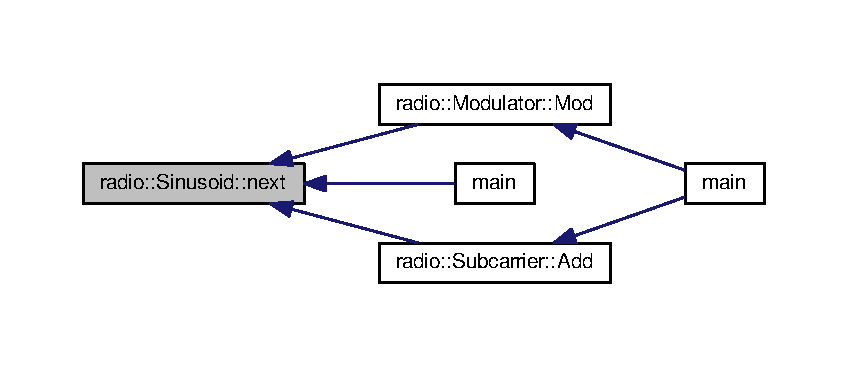
\includegraphics[width=350pt]{classradio_1_1Sinusoid_aab44298ea1bd5cb175d5826243cf56f2_icgraph}
\end{center}
\end{figure}


\hypertarget{classradio_1_1Sinusoid_a3f2741e9dd30291e5fa87f2eb2243e7c}{\index{radio\+::\+Sinusoid@{radio\+::\+Sinusoid}!next\+Shifted@{next\+Shifted}}
\index{next\+Shifted@{next\+Shifted}!radio\+::\+Sinusoid@{radio\+::\+Sinusoid}}
\subsubsection[{next\+Shifted}]{\setlength{\rightskip}{0pt plus 5cm}{\bf float32} radio\+::\+Sinusoid\+::next\+Shifted (
\begin{DoxyParamCaption}
{}
\end{DoxyParamCaption}
)}}\label{classradio_1_1Sinusoid_a3f2741e9dd30291e5fa87f2eb2243e7c}
Provides the next value of the shifted sinusoid in a manner consistant with a ring buffer. 

Definition at line \hyperlink{Sinusoid_8hpp_source_l00103}{103} of file \hyperlink{Sinusoid_8hpp_source}{Sinusoid.\+hpp}.



Here is the caller graph for this function\+:
\nopagebreak
\begin{figure}[H]
\begin{center}
\leavevmode
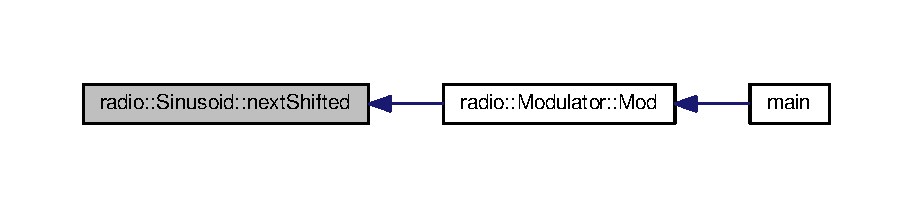
\includegraphics[width=350pt]{classradio_1_1Sinusoid_a3f2741e9dd30291e5fa87f2eb2243e7c_icgraph}
\end{center}
\end{figure}




\subsection{Member Data Documentation}
\hypertarget{classradio_1_1Sinusoid_ad429b5dd330e96aaf89a0d48ef59d3f2}{\index{radio\+::\+Sinusoid@{radio\+::\+Sinusoid}!frequency@{frequency}}
\index{frequency@{frequency}!radio\+::\+Sinusoid@{radio\+::\+Sinusoid}}
\subsubsection[{frequency}]{\setlength{\rightskip}{0pt plus 5cm}{\bf float32} radio\+::\+Sinusoid\+::frequency\hspace{0.3cm}{\ttfamily [protected]}}}\label{classradio_1_1Sinusoid_ad429b5dd330e96aaf89a0d48ef59d3f2}
The frequency of the sinusoid. 

Definition at line \hyperlink{Sinusoid_8hpp_source_l00049}{49} of file \hyperlink{Sinusoid_8hpp_source}{Sinusoid.\+hpp}.

\hypertarget{classradio_1_1Sinusoid_a964d64aae9acc4ea5d752534a33d76b8}{\index{radio\+::\+Sinusoid@{radio\+::\+Sinusoid}!sampling\+Rate@{sampling\+Rate}}
\index{sampling\+Rate@{sampling\+Rate}!radio\+::\+Sinusoid@{radio\+::\+Sinusoid}}
\subsubsection[{sampling\+Rate}]{\setlength{\rightskip}{0pt plus 5cm}{\bf uint32} radio\+::\+Sinusoid\+::sampling\+Rate\hspace{0.3cm}{\ttfamily [protected]}}}\label{classradio_1_1Sinusoid_a964d64aae9acc4ea5d752534a33d76b8}
The sampling rate. 

Definition at line \hyperlink{Sinusoid_8hpp_source_l00064}{64} of file \hyperlink{Sinusoid_8hpp_source}{Sinusoid.\+hpp}.

\hypertarget{classradio_1_1Sinusoid_a2e7d029c5e7307967c77959367cc0224}{\index{radio\+::\+Sinusoid@{radio\+::\+Sinusoid}!sin\+Index@{sin\+Index}}
\index{sin\+Index@{sin\+Index}!radio\+::\+Sinusoid@{radio\+::\+Sinusoid}}
\subsubsection[{sin\+Index}]{\setlength{\rightskip}{0pt plus 5cm}{\bf uint32} radio\+::\+Sinusoid\+::sin\+Index = 0\hspace{0.3cm}{\ttfamily [protected]}}}\label{classradio_1_1Sinusoid_a2e7d029c5e7307967c77959367cc0224}
The current index of the sinusoid's unshifted array. 

Definition at line \hyperlink{Sinusoid_8hpp_source_l00054}{54} of file \hyperlink{Sinusoid_8hpp_source}{Sinusoid.\+hpp}.

\hypertarget{classradio_1_1Sinusoid_a4acf2add824249c39046fe87f9a64f93}{\index{radio\+::\+Sinusoid@{radio\+::\+Sinusoid}!sin\+Index\+Shifted@{sin\+Index\+Shifted}}
\index{sin\+Index\+Shifted@{sin\+Index\+Shifted}!radio\+::\+Sinusoid@{radio\+::\+Sinusoid}}
\subsubsection[{sin\+Index\+Shifted}]{\setlength{\rightskip}{0pt plus 5cm}{\bf uint32} radio\+::\+Sinusoid\+::sin\+Index\+Shifted = 0\hspace{0.3cm}{\ttfamily [protected]}}}\label{classradio_1_1Sinusoid_a4acf2add824249c39046fe87f9a64f93}
The current index of the shifted sinusoid's array. 

Definition at line \hyperlink{Sinusoid_8hpp_source_l00059}{59} of file \hyperlink{Sinusoid_8hpp_source}{Sinusoid.\+hpp}.

\hypertarget{classradio_1_1Sinusoid_a56556c3d3e08d1c9481c18e087ff1c85}{\index{radio\+::\+Sinusoid@{radio\+::\+Sinusoid}!sinusoid@{sinusoid}}
\index{sinusoid@{sinusoid}!radio\+::\+Sinusoid@{radio\+::\+Sinusoid}}
\subsubsection[{sinusoid}]{\setlength{\rightskip}{0pt plus 5cm}{\bf float32}$\ast$ radio\+::\+Sinusoid\+::sinusoid\hspace{0.3cm}{\ttfamily [protected]}}}\label{classradio_1_1Sinusoid_a56556c3d3e08d1c9481c18e087ff1c85}
Initialized as an array of the sinusoid values. 

Definition at line \hyperlink{Sinusoid_8hpp_source_l00069}{69} of file \hyperlink{Sinusoid_8hpp_source}{Sinusoid.\+hpp}.

\hypertarget{classradio_1_1Sinusoid_a556db1dca1d5af3d9c6ba2d51f9e3cf8}{\index{radio\+::\+Sinusoid@{radio\+::\+Sinusoid}!sinusoid\+Shift90@{sinusoid\+Shift90}}
\index{sinusoid\+Shift90@{sinusoid\+Shift90}!radio\+::\+Sinusoid@{radio\+::\+Sinusoid}}
\subsubsection[{sinusoid\+Shift90}]{\setlength{\rightskip}{0pt plus 5cm}{\bf float32}$\ast$ radio\+::\+Sinusoid\+::sinusoid\+Shift90\hspace{0.3cm}{\ttfamily [protected]}}}\label{classradio_1_1Sinusoid_a556db1dca1d5af3d9c6ba2d51f9e3cf8}
Initialized as an array of the sinusoid values shifted 90 degrees. 

Definition at line \hyperlink{Sinusoid_8hpp_source_l00075}{75} of file \hyperlink{Sinusoid_8hpp_source}{Sinusoid.\+hpp}.



The documentation for this class was generated from the following file\+:\begin{DoxyCompactItemize}
\item 
src/\hyperlink{Sinusoid_8hpp}{Sinusoid.\+hpp}\end{DoxyCompactItemize}

\chapter{File Documentation}
\hypertarget{bbftest}{\section{bin/bbftest File Reference}
\label{bbftest}\index{bin/bbftest@{bin/bbftest}}
}


\subsection{Detailed Description}
\begin{DoxyAuthor}{Author}
Samuel Andrew Wisner, \href{mailto:awisner94@gmail.com}{\tt awisner94@gmail.\+com} 
\end{DoxyAuthor}


Definition in file \hyperlink{bbftest_source}{bbftest}.


\hypertarget{bbftest_source}{\section{bbftest}
\label{bbftest_source}\index{bin/bbftest@{bin/bbftest}}
}

\begin{DoxyCode}
00001 basebandfiltertest | aplay -c 2 -r 48000 -t raw -f S32\_LE
\end{DoxyCode}

\hypertarget{lsbftest}{\section{bin/lsbftest File Reference}
\label{lsbftest}\index{bin/lsbftest@{bin/lsbftest}}
}


Runs test on the L\+S\+B filter.  




\subsection{Detailed Description}
Runs test on the L\+S\+B filter. 

\begin{DoxyAuthor}{Author}
Samuel Andrew Wisner, \href{mailto:awisner94@gmail.com}{\tt awisner94@gmail.\+com} 
\end{DoxyAuthor}


Definition in file \hyperlink{lsbftest_source}{lsbftest}.


\hypertarget{lsbftest_source}{\section{lsbftest}
\label{lsbftest_source}\index{bin/lsbftest@{bin/lsbftest}}
}

\begin{DoxyCode}
00001 lowersidebandftest | aplay -c 2 -r 48000 -t raw -f S32\_LE
\end{DoxyCode}

\hypertarget{modtest}{\section{bin/modtest File Reference}
\label{modtest}\index{bin/modtest@{bin/modtest}}
}


Runs test on the modulation of a simple sinusoid.  




\subsection{Detailed Description}
Runs test on the modulation of a simple sinusoid. 

\begin{DoxyAuthor}{Author}
Samuel Andrew Wisner, \href{mailto:awisner94@gmail.com}{\tt awisner94@gmail.\+com} 
\end{DoxyAuthor}


Definition in file \hyperlink{modtest_source}{modtest}.


\hypertarget{modtest_source}{\section{modtest}
\label{modtest_source}\index{bin/modtest@{bin/modtest}}
}

\begin{DoxyCode}
00001 OPTIONS="-c 2 -r 48000 -t raw -f S32\_LE -q"
00002 modulatortest $1 $2 $3 | aplay $OPTIONS -D plughw:0,0
\end{DoxyCode}

\hypertarget{msintest}{\section{bin/msintest File Reference}
\label{msintest}\index{bin/msintest@{bin/msintest}}
}


Runs test involving the generation of many sinusoids.  




\subsection{Detailed Description}
Runs test involving the generation of many sinusoids. 

\begin{DoxyAuthor}{Author}
Samuel Andrew Wisner, \href{mailto:awisner94@gmail.com}{\tt awisner94@gmail.\+com} 
\end{DoxyAuthor}


Definition in file \hyperlink{msintest_source}{msintest}.


\hypertarget{msintest_source}{\section{msintest}
\label{msintest_source}\index{bin/msintest@{bin/msintest}}
}

\begin{DoxyCode}
00001 multisinusoidtest | aplay -c 2 -r 48000 -t raw -f S32\_LE
\end{DoxyCode}

\hypertarget{pltest}{\section{bin/pltest File Reference}
\label{pltest}\index{bin/pltest@{bin/pltest}}
}


\subsection{Detailed Description}
\begin{DoxyAuthor}{Author}
Samuel Andrew Wisner, \href{mailto:awisner94@gmail.com}{\tt awisner94@gmail.\+com} 
\end{DoxyAuthor}


Definition in file \hyperlink{pltest_source}{pltest}.


\hypertarget{pltest_source}{\section{pltest}
\label{pltest_source}\index{bin/pltest@{bin/pltest}}
}

\begin{DoxyCode}
00001 OPTIONS="-c 2 -r 48000 -t raw -f S32\_LE"
00002 pltonetest $1 | aplay $OPTIONS
\end{DoxyCode}

\hypertarget{radio}{\section{bin/radio File Reference}
\label{radio}\index{bin/radio@{bin/radio}}
}


The main program's script. Call this script to modulate audio!  




\subsection{Detailed Description}
The main program's script. Call this script to modulate audio! 

\begin{DoxyAuthor}{Author}
Samuel Andrew Wisner, \href{mailto:awisner94@gmail.com}{\tt awisner94@gmail.\+com} 
\end{DoxyAuthor}


Definition in file \hyperlink{radio_source}{radio}.


\hypertarget{radio_source}{\section{radio}
\label{radio_source}\index{bin/radio@{bin/radio}}
}

\begin{DoxyCode}
00001 OPTIONS="-r 48000 -t raw -q"
00002 arecord $OPTIONS -c 1 -D plughw:1,0 -f FLOAT\_LE | sdr $1 $2 $3 | \(\backslash\)
00003 aplay $OPTIONS -c 2 -f S32\_LE -D plughw:0,0
\end{DoxyCode}

\hypertarget{sintest}{\section{bin/sintest File Reference}
\label{sintest}\index{bin/sintest@{bin/sintest}}
}


Runs a test on the Sinusoid class.  




\subsection{Detailed Description}
Runs a test on the Sinusoid class. 

\begin{DoxyAuthor}{Author}
Samuel Andrew Wisner, \href{mailto:awisner94@gmail.com}{\tt awisner94@gmail.\+com} 
\end{DoxyAuthor}


Definition in file \hyperlink{sintest_source}{sintest}.


\hypertarget{sintest_source}{\section{sintest}
\label{sintest_source}\index{bin/sintest@{bin/sintest}}
}

\begin{DoxyCode}
00001 OPTIONS="-c 2 -r 48000 -t raw -f S32\_LE"
00002 sinusoidtest $1 | aplay $OPTIONS
\end{DoxyCode}

\hypertarget{usbftest}{\section{bin/usbftest File Reference}
\label{usbftest}\index{bin/usbftest@{bin/usbftest}}
}


\subsection{Detailed Description}
\begin{DoxyAuthor}{Author}
Samuel Andrew Wisner, \href{mailto:awisner94@gmail.com}{\tt awisner94@gmail.\+com} 
\end{DoxyAuthor}


Definition in file \hyperlink{usbftest_source}{usbftest}.


\hypertarget{usbftest_source}{\section{usbftest}
\label{usbftest_source}\index{bin/usbftest@{bin/usbftest}}
}

\begin{DoxyCode}
00001 uppersidebandftest | aplay -c 2 -r 48000 -t raw -f S32\_LE
\end{DoxyCode}

\hypertarget{doxygen_8config}{\section{etc/doxygen.config File Reference}
\label{doxygen_8config}\index{etc/doxygen.\+config@{etc/doxygen.\+config}}
}


Contains doxygen configuration.  




\subsection{Detailed Description}
Contains doxygen configuration. 

\begin{DoxyAuthor}{Author}
Samuel Andrew Wisner, \href{mailto:awisner94@gmail.com}{\tt awisner94@gmail.\+com} 
\end{DoxyAuthor}


Definition in file \hyperlink{doxygen_8config_source}{doxygen.\+config}.


\hypertarget{doxygen_8config_source}{\section{doxygen.\+config}
\label{doxygen_8config_source}\index{etc/doxygen.\+config@{etc/doxygen.\+config}}
}

\begin{DoxyCode}
00001 PROJECT\_NAME = "An Inexpensive, Software-Defined IF Modulator"
00002 
00003 INPUT = makefile src/ etc/doxygen.config bin/bbftest bin/modtest bin/msintest bin/lsbftest bin/pltest
       bin/radio bin/sintest bin/usbftest
00004 OUTPUT\_DIRECTORY = doc/
00005 
00006 GENERATE\_HTML = YES
00007 GENERATE\_RTF = YES
00008 GENERATE\_LATEX = YES
00009 GENERATE\_MAN = YES
00010 GENERATE\_XML = NO
00011 GENERATE\_DOCBOOK = NO
00012 
00013 USE\_PDF\_LATEX = YES
00014 USE\_PDF\_HYPERLINKS = YES
00015 
00016 RECURSIVE = YES
00017 SOURCE\_BROWSER = YES
00018 SOURCE\_TOOLTIPS = YES
00019 EXTRACT\_ALL = YES
00020 DISABLE\_INDEX = NO
00021 GENERATE\_TREEVIEW = YES
00022 SEARCHENGINE = YES
00023 SERVER\_BASED\_SEARCH = NO
00024 
00025 LATEX\_SOURCE\_CODE = YES
00026 STRIP\_CODE\_COMMENTS = YES
00027 INLINE\_SOURCES = NO
00028 
00029 HAVE\_DOT = YES
00030 CALL\_GRAPH = YES
00031 CALLER\_GRAPH = YES
\end{DoxyCode}

\hypertarget{makefile}{\section{makefile File Reference}
\label{makefile}\index{makefile@{makefile}}
}

\hypertarget{makefile_source}{\section{makefile}
}

\begin{DoxyCode}
00001 GCC = g++ -g -std=gnu++14
00002 
00003 alsa-test:
00004    $(GCC) src/alsa\_test.cpp -o bin/alsatest -O0 -lasound
00005 
00006 baseband-filter-test:
00007    $(GCC) src/baseband\_filter\_test.cpp -o bin/basebandfiltertest
00008 
00009 count:
00010    grep -r "src/" -e "Samuel Andrew Wisner" -l | xargs wc -l
00011 
00012 docs:
00013    rm -r doc/
00014    doxygen etc/doxygen.config
00015    cd doc/latex; make pdf;
00016    git reset
00017    git add doc/.
00018    git --no-pager log > etc/log.txt
00019    git add etc/log.txt
00020    git commit -m "Updated documentation."
00021    git push
00022 
00023 fft-test:
00024    $(GCC) src/fft\_test.cpp -o bin/fft-test
00025 
00026 fft-test2:
00027    $(GCC) src/fft\_test2.cpp -o bin/fft-test2
00028 
00029 iq-test:
00030    $(GCC) src/iq\_test.cpp -o bin/iqtest
00031 
00032 multi-sinusoid-test:
00033    $(GCC) src/multi\_sinusoid\_test.cpp -o bin/multisinusoidtest
00034 
00035 modulator-test:
00036    $(GCC) src/modulator\_test.cpp -o bin/modulatortest
00037 
00038 lsb-filter-test:
00039    $(GCC) src/lsb\_filter\_test.cpp -o bin/lowersidebandftest
00040 
00041 pl-tone-test:
00042    $(GCC) src/pl\_tone\_test.cpp -o bin/pltonetest
00043 
00044 radio:
00045    $(GCC) src/main.cpp -o bin/sdr
00046 
00047 sinusoid-test:
00048    $(GCC) src/sinusoid\_test.cpp -o bin/sinusoidtest
00049 
00050 usb-filter-test:
00051    $(GCC) src/usb\_filter\_test.cpp -o bin/uppersidebandftest
00052 
00053 
\end{DoxyCode}

\hypertarget{alsa__test_8cpp}{\section{src/alsa\+\_\+test.cpp File Reference}
\label{alsa__test_8cpp}\index{src/alsa\+\_\+test.\+cpp@{src/alsa\+\_\+test.\+cpp}}
}


Tests sinusoidal tone generation.  


{\ttfamily \#include $<$cmath$>$}\\*
{\ttfamily \#include $<$climits$>$}\\*
{\ttfamily \#include $<$iostream$>$}\\*
{\ttfamily \#include $<$alsa/asoundlib.\+h$>$}\\*
{\ttfamily \#include \char`\"{}definitions.\+hpp\char`\"{}}\\*
Include dependency graph for alsa\+\_\+test.\+cpp\+:
\nopagebreak
\begin{figure}[H]
\begin{center}
\leavevmode
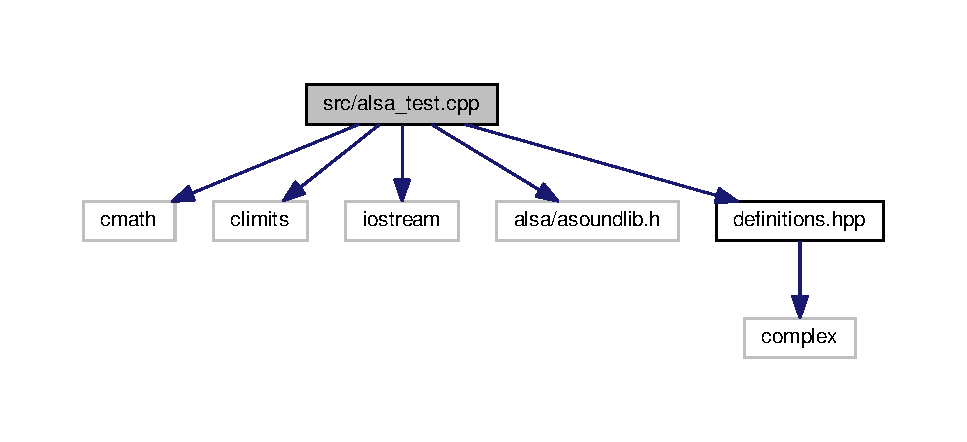
\includegraphics[width=350pt]{alsa__test_8cpp__incl}
\end{center}
\end{figure}
\subsection*{Functions}
\begin{DoxyCompactItemize}
\item 
int \hyperlink{alsa__test_8cpp_ae66f6b31b5ad750f1fe042a706a4e3d4}{main} ()
\end{DoxyCompactItemize}


\subsection{Detailed Description}
Tests sinusoidal tone generation. 

\begin{DoxyAuthor}{Author}
Samuel Andrew Wisner, \href{mailto:awisner94@gmail.com}{\tt awisner94@gmail.\+com} 
\end{DoxyAuthor}
\begin{DoxyRefDesc}{Bug}
\item[\hyperlink{bug__bug000001}{Bug}]Clicking noise from sinusoidal discontinuity \end{DoxyRefDesc}


Definition in file \hyperlink{alsa__test_8cpp_source}{alsa\+\_\+test.\+cpp}.



\subsection{Function Documentation}
\hypertarget{alsa__test_8cpp_ae66f6b31b5ad750f1fe042a706a4e3d4}{\index{alsa\+\_\+test.\+cpp@{alsa\+\_\+test.\+cpp}!main@{main}}
\index{main@{main}!alsa\+\_\+test.\+cpp@{alsa\+\_\+test.\+cpp}}
\subsubsection[{main}]{\setlength{\rightskip}{0pt plus 5cm}int main (
\begin{DoxyParamCaption}
{}
\end{DoxyParamCaption}
)}}\label{alsa__test_8cpp_ae66f6b31b5ad750f1fe042a706a4e3d4}
This program tests sinusoidal speaker output through the A\+L\+S\+A A\+P\+I. Not sure if it works. When it did at least compile and run, it produced a sinusoid with an approximately twice-\/per-\/second clicking noise. 

Definition at line \hyperlink{alsa__test_8cpp_source_l00022}{22} of file \hyperlink{alsa__test_8cpp_source}{alsa\+\_\+test.\+cpp}.


\hypertarget{alsa__test_8cpp_source}{\section{alsa\+\_\+test.\+cpp}
\label{alsa__test_8cpp_source}\index{src/alsa\+\_\+test.\+cpp@{src/alsa\+\_\+test.\+cpp}}
}

\begin{DoxyCode}
00001 
00008 \textcolor{preprocessor}{#include <cmath>}
00009 \textcolor{preprocessor}{#include <climits>}
00010 \textcolor{preprocessor}{#include <iostream>}
00011 \textcolor{preprocessor}{#include <alsa/asoundlib.h>}
00012 
00013 \textcolor{preprocessor}{#include "\hyperlink{definitions_8hpp}{definitions.hpp}"}
00014 
00015 \textcolor{keyword}{using namespace }\hyperlink{namespacestd}{std};
00016 
\hypertarget{alsa__test_8cpp_source_l00022}{}\hyperlink{alsa__test_8cpp_ae66f6b31b5ad750f1fe042a706a4e3d4}{00022} \textcolor{keywordtype}{int} \hyperlink{alsa__test_8cpp_ae66f6b31b5ad750f1fe042a706a4e3d4}{main}() \{
00023     \textcolor{keywordtype}{int} ret;
00024 
00025     snd\_pcm\_t* pcm\_handle;  \textcolor{comment}{// device handle}
00026     snd\_pcm\_stream\_t stream = SND\_PCM\_STREAM\_PLAYBACK;
00027     snd\_pcm\_hw\_params\_t* hwparams;  \textcolor{comment}{// hardware information}
00028     \textcolor{keywordtype}{char}* pcm\_name = strdup(\textcolor{stringliteral}{"plughw:1,0"});  \textcolor{comment}{// on-board audio jack}
00029     \textcolor{keywordtype}{int} rate = 48000;
00030 
00031     \textcolor{keyword}{const} \hyperlink{definitions_8hpp_a05f6b0ae8f6a6e135b0e290c25fe0e4e}{uint16} freq = 440;
00032     \textcolor{keywordtype}{long} \textcolor{keywordtype}{unsigned} \textcolor{keywordtype}{int} bufferSize = 4096*4;  \textcolor{comment}{// anything >8192 causes seg fault}
00033     \textcolor{keyword}{const} \hyperlink{definitions_8hpp_a1134b580f8da4de94ca6b1de4d37975e}{uint32} len = bufferSize*100;
00034     \textcolor{keyword}{const} \hyperlink{definitions_8hpp_aacdc525d6f7bddb3ae95d5c311bd06a1}{float32} arg = 2 * 3.141592 * freq / rate;
00035     \hyperlink{definitions_8hpp_a74df79fde3c518e55b29ce6360a9c76e}{sint16} vals[len];
00036 
00037     \textcolor{keywordtype}{long} \textcolor{keywordtype}{unsigned} \textcolor{keywordtype}{int} count = 0;
00038 
00039     \textcolor{keywordflow}{for}(\hyperlink{definitions_8hpp_a1134b580f8da4de94ca6b1de4d37975e}{uint32} i = 0; i < len; i = i + 2) \{
00040         vals[i] = (\hyperlink{definitions_8hpp_a74df79fde3c518e55b29ce6360a9c76e}{sint16})(SHRT\_MAX * cos(arg * i/2) + 0.5);
00041         vals[i+1] = vals[i];
00042     \}
00043 
00044     ret = snd\_pcm\_open(&pcm\_handle, pcm\_name, stream, 0);
00045     cout << \textcolor{stringliteral}{"Opening: "} << snd\_strerror(ret) << endl;
00046 
00047     ret = snd\_pcm\_hw\_params\_any(pcm\_handle, hwparams);
00048     cout << \textcolor{stringliteral}{"Initializing hwparams structure: "} << snd\_strerror(ret) << endl;   
00049 
00050     ret = snd\_pcm\_hw\_params\_set\_access(pcm\_handle, hwparams,
00051             SND\_PCM\_ACCESS\_RW\_INTERLEAVED);
00052     cout << \textcolor{stringliteral}{"Setting access: "} << snd\_strerror(ret) << endl;
00053 
00054     ret = snd\_pcm\_hw\_params\_set\_format(pcm\_handle, hwparams,
00055             SND\_PCM\_FORMAT\_S16\_LE);
00056     cout << \textcolor{stringliteral}{"Setting format: "} << snd\_strerror(ret) << endl;
00057 
00058     ret = snd\_pcm\_hw\_params\_set\_rate(pcm\_handle, hwparams,
00059             rate, (\textcolor{keywordtype}{int})0);
00060     cout << \textcolor{stringliteral}{"Setting rate: "} << snd\_strerror(ret) << endl;
00061 
00062     ret = snd\_pcm\_hw\_params\_set\_channels(pcm\_handle, hwparams, 2); 
00063     cout << \textcolor{stringliteral}{"Setting channels: "} << snd\_strerror(ret) << endl;
00064 
00065     ret = snd\_pcm\_hw\_params\_set\_periods(pcm\_handle, hwparams, 2, 0);
00066     cout << \textcolor{stringliteral}{"Setting periods: "} << snd\_strerror(ret) << endl;
00067 
00068     ret = snd\_pcm\_hw\_params\_set\_buffer\_size\_near(pcm\_handle, hwparams,
00069             &bufferSize);
00070     cout << \textcolor{stringliteral}{"Setting buffer size: "} << snd\_strerror(ret) << endl;
00071 
00072     ret = snd\_pcm\_hw\_params(pcm\_handle, hwparams);
00073     cout << \textcolor{stringliteral}{"Applying parameters: "} << snd\_strerror(ret) << endl;
00074 
00075 \textcolor{comment}{//  ret = snd\_pcm\_hw\_params\_get\_period\_size(hwparams, &count, 0);}
00076     cout << \textcolor{stringliteral}{"Actual period size: "} << count << endl;
00077     cout << \textcolor{stringliteral}{"Returned: "} << snd\_strerror(ret) << endl;
00078 
00079 
00080 
00081     cout << endl << endl;
00082 
00083 
00084     \textcolor{keyword}{const} \textcolor{keywordtype}{void}* ptr[100];
00085 
00086     \textcolor{keywordflow}{for}(\textcolor{keywordtype}{int} i = 0; i < 100; i++) \{
00087         ptr[i] = (\textcolor{keyword}{const} \textcolor{keywordtype}{void}*)&vals + bufferSize*i;
00088     \}
00089 
00090     \textcolor{keywordtype}{int} err;
00091 
00092     \textcolor{keywordflow}{for}(\textcolor{keywordtype}{int} i = 0; i < 100; i++) \{
00093         \textcolor{keywordflow}{do} \{
00094             ret = snd\_pcm\_writei(pcm\_handle,
00095                     ptr[i], count);
00096 
00097             \textcolor{keywordflow}{if}(ret < 0) \{
00098                 err = snd\_pcm\_prepare(pcm\_handle);
00099                 cout << \textcolor{stringliteral}{"Preparing: "} << snd\_strerror(err)
00100                     << endl;
00101             \}
00102         \} \textcolor{keywordflow}{while}(ret < 0);
00103 
00104         cout << \textcolor{stringliteral}{"Writing data: "} << ret << endl;
00105     \}
00106 \}
\end{DoxyCode}

\hypertarget{auxiliary_8hpp}{\section{src/auxiliary.hpp File Reference}
\label{auxiliary_8hpp}\index{src/auxiliary.\+hpp@{src/auxiliary.\+hpp}}
}


Contains helper-\/functions for \hyperlink{alsa__test_8cpp_ae66f6b31b5ad750f1fe042a706a4e3d4}{main()}.  


{\ttfamily \#include $<$climits$>$}\\*
{\ttfamily \#include $<$iostream$>$}\\*
{\ttfamily \#include $<$stdexcept$>$}\\*
{\ttfamily \#include $<$string$>$}\\*
{\ttfamily \#include \char`\"{}definitions.\+hpp\char`\"{}}\\*
Include dependency graph for auxiliary.\+hpp\+:
\nopagebreak
\begin{figure}[H]
\begin{center}
\leavevmode
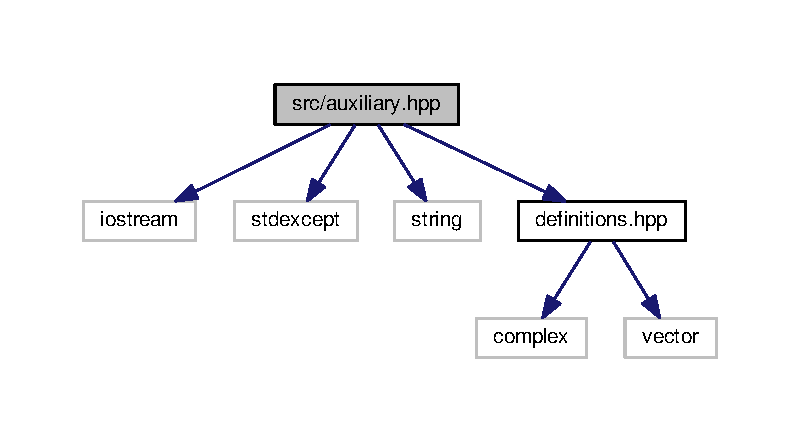
\includegraphics[width=350pt]{auxiliary_8hpp__incl}
\end{center}
\end{figure}
This graph shows which files directly or indirectly include this file\+:
\nopagebreak
\begin{figure}[H]
\begin{center}
\leavevmode
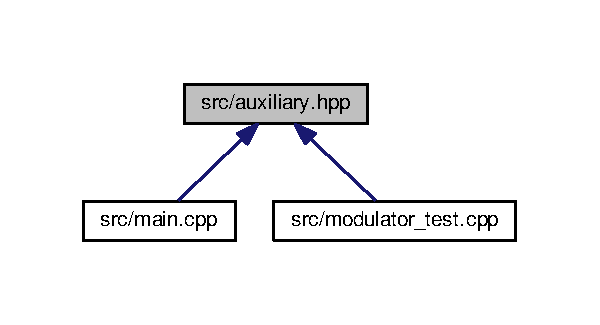
\includegraphics[width=350pt]{auxiliary_8hpp__dep__incl}
\end{center}
\end{figure}
\subsection*{Namespaces}
\begin{DoxyCompactItemize}
\item 
 \hyperlink{namespaceradio}{radio}
\end{DoxyCompactItemize}
\subsection*{Functions}
\begin{DoxyCompactItemize}
\item 
void \hyperlink{namespaceradio_a6db7c682d0f9aeac8cb5042717b8ae7f}{radio\+::\+Show\+Help} ()
\item 
void \hyperlink{namespaceradio_ae4b2334c4366dcdf0311ad79d2067945}{radio\+::to\+\_\+sint32} (\hyperlink{definitions_8hpp_aacdc525d6f7bddb3ae95d5c311bd06a1}{float32} $\ast$data, \hyperlink{definitions_8hpp_a1134b580f8da4de94ca6b1de4d37975e}{uint32} size)
\item 
Modulation\+Type \hyperlink{namespaceradio_a402fe28e2e2bb2be7a0d2d9f74cc640d}{radio\+::to\+\_\+type} (std\+::string str)
\end{DoxyCompactItemize}


\subsection{Detailed Description}
Contains helper-\/functions for \hyperlink{alsa__test_8cpp_ae66f6b31b5ad750f1fe042a706a4e3d4}{main()}. 

\begin{DoxyAuthor}{Author}
Samuel Andrew Wisner, \href{mailto:awisner94@gmail.com}{\tt awisner94@gmail.\+com} 
\end{DoxyAuthor}


Definition in file \hyperlink{auxiliary_8hpp_source}{auxiliary.\+hpp}.


\hypertarget{auxiliary_8hpp_source}{\section{auxiliary.\+hpp}
\label{auxiliary_8hpp_source}\index{src/auxiliary.\+hpp@{src/auxiliary.\+hpp}}
}

\begin{DoxyCode}
00001 
00007 \textcolor{preprocessor}{#ifndef auxiliary\_H}
00008 \textcolor{preprocessor}{#define auxiliary\_H}
00009 
00010 \textcolor{preprocessor}{#include <climits>}
00011 \textcolor{preprocessor}{#include <iostream>}
00012 \textcolor{preprocessor}{#include <stdexcept>}
00013 \textcolor{preprocessor}{#include <string>}
00014 
00015 \textcolor{preprocessor}{#include "\hyperlink{definitions_8hpp}{definitions.hpp}"}
00016 
\hypertarget{auxiliary_8hpp_source_l00017}{}\hyperlink{namespaceradio}{00017} \textcolor{keyword}{namespace }\hyperlink{namespaceradio}{radio} \{
00018 
\hypertarget{auxiliary_8hpp_source_l00022}{}\hyperlink{namespaceradio_a6db7c682d0f9aeac8cb5042717b8ae7f}{00022}     \textcolor{keywordtype}{void} \hyperlink{namespaceradio_a6db7c682d0f9aeac8cb5042717b8ae7f}{ShowHelp}() \{
00023         std::cerr << std::endl << \textcolor{stringliteral}{"Usage: radio [MODE] [MIC GAIN] "}
00024             \textcolor{stringliteral}{"[PL TONE]"} << std::endl << std::endl
00025             << \textcolor{stringliteral}{"MODE: one of the following types "}
00026             \textcolor{stringliteral}{"of modulation"} << std::endl << std::endl;
00027 
00028         std::cerr << \textcolor{stringliteral}{"dsblc\(\backslash\)t\(\backslash\)tDouble sideband, large carrier"} << std::endl
00029             << \textcolor{stringliteral}{"am\(\backslash\)t\(\backslash\)tAlias for dsblc"} << std::endl
00030             << \textcolor{stringliteral}{"dsbsc\(\backslash\)t\(\backslash\)tDouble sideband, suppressed carrier"} << std::endl
00031             << \textcolor{stringliteral}{"lsbhil\(\backslash\)t\(\backslash\)tLower sideband created via Hilbert transform"}
00032             << std::endl
00033             << \textcolor{stringliteral}{"lsbfilt\(\backslash\)t\(\backslash\)tLower sideband created via digital low-pass filter"}
00034             << std::endl
00035             << \textcolor{stringliteral}{"usbhil\(\backslash\)t\(\backslash\)tUpper sideband created via Hilbert transform"}
00036             << std::endl
00037             << \textcolor{stringliteral}{"usbfilt\(\backslash\)t\(\backslash\)tUpper sideband created via digital high-pass filter"}
00038             << std::endl
00039 \textcolor{comment}{//          << "nfm\(\backslash\)t\(\backslash\)tFrequency modulation, 2.5 kHz bandwidth"}
00040             << std::endl;
00041 \textcolor{comment}{//          << "wfm\(\backslash\)t\(\backslash\)tFrequency modulation, 5 kHz bandwidth" << std::endl}
00042 \textcolor{comment}{//          << "fm\(\backslash\)t\(\backslash\)talias for wfm" << std::endl << std::endl;}
00043 
00044         std::cerr << \textcolor{stringliteral}{"MIC GAIN: Microphone power gain expressed in decibels"}
00045         << std::endl << std::endl;
00046 
00047         std::cerr << \textcolor{stringliteral}{"PL TONE: Optional specification for CTCSS tone from "}
00048             \textcolor{stringliteral}{"60-260 Hz"} << std::endl << std::endl;
00049 
00050         std::exit(\hyperlink{definitions_8hpp_a8fe83ac76edc595f6b98cd4a4127aed5}{ERROR});
00051     \}
00052 
\hypertarget{auxiliary_8hpp_source_l00062}{}\hyperlink{namespaceradio_ae4b2334c4366dcdf0311ad79d2067945}{00062}     \textcolor{keywordtype}{void} \hyperlink{namespaceradio_ae4b2334c4366dcdf0311ad79d2067945}{to\_sint32}(\hyperlink{definitions_8hpp_aacdc525d6f7bddb3ae95d5c311bd06a1}{float32}* data, \hyperlink{definitions_8hpp_a1134b580f8da4de94ca6b1de4d37975e}{uint32} size) \{
00063         \textcolor{keywordflow}{for}(\hyperlink{definitions_8hpp_a1134b580f8da4de94ca6b1de4d37975e}{uint32} i = 0; i < size; i++) \{
00064             ((\hyperlink{definitions_8hpp_a0573de65958b4fda3a0460ed417dafb8}{sint32}*)data)[i] = (\hyperlink{definitions_8hpp_a0573de65958b4fda3a0460ed417dafb8}{sint32})(data[i] * INT\_MAX + 0.5);
00065         \}
00066     \}
00067 
\hypertarget{auxiliary_8hpp_source_l00080}{}\hyperlink{namespaceradio_a402fe28e2e2bb2be7a0d2d9f74cc640d}{00080}     \hyperlink{namespaceradio_a46fb7299001138f28b7f69975c58399e}{ModulationType} \hyperlink{namespaceradio_a402fe28e2e2bb2be7a0d2d9f74cc640d}{to\_type}(std::string str) \{
00081         \hyperlink{namespaceradio_a46fb7299001138f28b7f69975c58399e}{ModulationType} type;
00082 
00083         \textcolor{keywordflow}{if}(str == \textcolor{stringliteral}{"dsblc"} || str == \textcolor{stringliteral}{"am"}) \{
00084             type = \hyperlink{namespaceradio_a46fb7299001138f28b7f69975c58399eaf180dafbc98f54c6382ae29243cec902}{ModulationType::DSB\_LC};
00085         \} \textcolor{keywordflow}{else} \textcolor{keywordflow}{if}(str == \textcolor{stringliteral}{"dsbsc"}) \{
00086             type = \hyperlink{namespaceradio_a46fb7299001138f28b7f69975c58399ea92c257208ae8b0c6d88c80abcf15ec31}{ModulationType::DSB\_SC};
00087         \} \textcolor{keywordflow}{else} \textcolor{keywordflow}{if}(str == \textcolor{stringliteral}{"lsbhil"}) \{
00088             type = \hyperlink{namespaceradio_a46fb7299001138f28b7f69975c58399ea18f970daa5b5a8f72cbd45f7b49a6b6a}{ModulationType::LSB\_HILBERT};
00089         \} \textcolor{keywordflow}{else} \textcolor{keywordflow}{if}(str == \textcolor{stringliteral}{"lsbfilt"}) \{
00090             type = \hyperlink{namespaceradio_a46fb7299001138f28b7f69975c58399eaa6fd9ffa81c9d5e4a255b0c3b2336bd8}{ModulationType::LSB\_FILTERED};
00091         \} \textcolor{keywordflow}{else} \textcolor{keywordflow}{if}(str == \textcolor{stringliteral}{"usbhil"}) \{
00092             type = \hyperlink{namespaceradio_a46fb7299001138f28b7f69975c58399ea1b14284e455bf5c311de662665312d13}{ModulationType::USB\_HILBERT};
00093         \} \textcolor{keywordflow}{else} \textcolor{keywordflow}{if}(str == \textcolor{stringliteral}{"usbfilt"}) \{
00094             type = \hyperlink{namespaceradio_a46fb7299001138f28b7f69975c58399ea9d8eca0470206cddb0dd0297717eb876}{ModulationType::USB\_FILTERED};
00095         \} \textcolor{keywordflow}{else} \textcolor{keywordflow}{if}(str == \textcolor{stringliteral}{"wfm"} || str == \textcolor{stringliteral}{"fm"}) \{
00096             type = \hyperlink{namespaceradio_a46fb7299001138f28b7f69975c58399ea7b4b1e7876b8d9de5b77b9264fbe556a}{ModulationType::FM\_NARROW};
00097         \} \textcolor{keywordflow}{else} \textcolor{keywordflow}{if}(str == \textcolor{stringliteral}{"nfm"}) \{
00098             type = \hyperlink{namespaceradio_a46fb7299001138f28b7f69975c58399eafabee3b32b363b14950cb5f5b61e998c}{ModulationType::FM\_WIDE};
00099         \} \textcolor{keywordflow}{else} \{
00100             \textcolor{keywordflow}{throw} std::logic\_error(\textcolor{stringliteral}{"The given modulation type is invalid!"});
00101         \}
00102 
00103         \textcolor{keywordflow}{return} type;
00104     \}
00105 \}
00106 
00107 \textcolor{preprocessor}{#endif}
\end{DoxyCode}

\hypertarget{baseband__filter__test_8cpp}{\section{src/baseband\+\_\+filter\+\_\+test.cpp File Reference}
\label{baseband__filter__test_8cpp}\index{src/baseband\+\_\+filter\+\_\+test.\+cpp@{src/baseband\+\_\+filter\+\_\+test.\+cpp}}
}


Tests sinusoidal tone generation.  


{\ttfamily \#include $<$iostream$>$}\\*
{\ttfamily \#include $<$cmath$>$}\\*
{\ttfamily \#include $<$cstdio$>$}\\*
{\ttfamily \#include $<$unistd.\+h$>$}\\*
{\ttfamily \#include \char`\"{}definitions.\+hpp\char`\"{}}\\*
{\ttfamily \#include \char`\"{}Filter.\+hpp\char`\"{}}\\*
{\ttfamily \#include \char`\"{}fvectors.\+hpp\char`\"{}}\\*
{\ttfamily \#include \char`\"{}zdomain.\+hpp\char`\"{}}\\*
Include dependency graph for baseband\+\_\+filter\+\_\+test.\+cpp\+:
\nopagebreak
\begin{figure}[H]
\begin{center}
\leavevmode
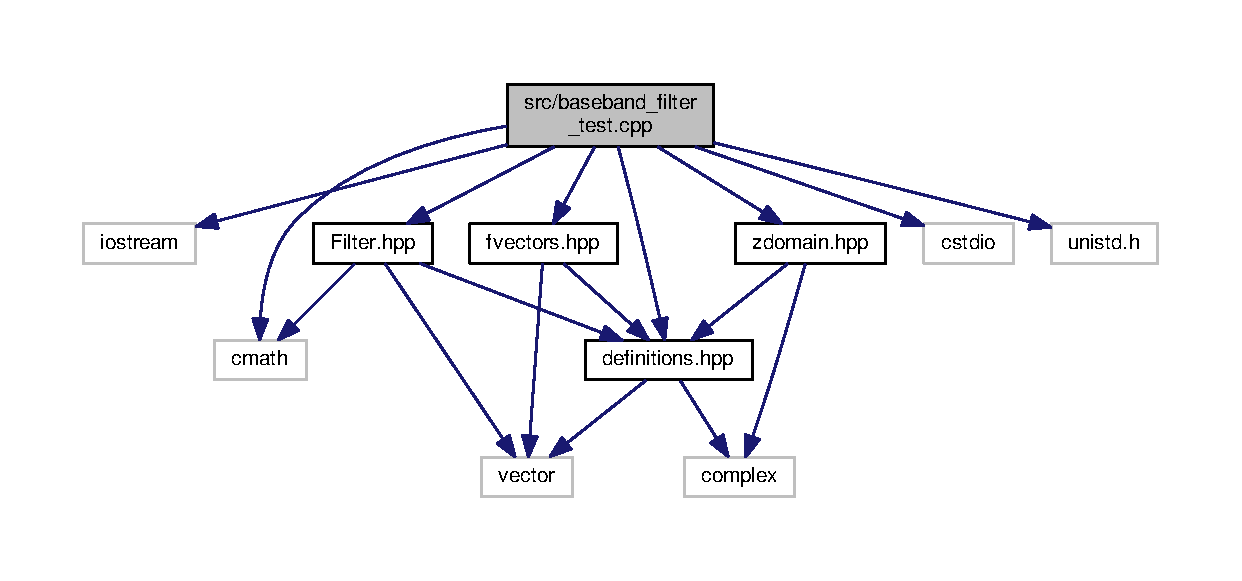
\includegraphics[width=350pt]{baseband__filter__test_8cpp__incl}
\end{center}
\end{figure}
\subsection*{Functions}
\begin{DoxyCompactItemize}
\item 
int \hyperlink{baseband__filter__test_8cpp_ae66f6b31b5ad750f1fe042a706a4e3d4}{main} ()
\end{DoxyCompactItemize}


\subsection{Detailed Description}
Tests sinusoidal tone generation. 

\begin{DoxyAuthor}{Author}
Samuel Andrew Wisner, \href{mailto:awisner94@gmail.com}{\tt awisner94@gmail.\+com} 
\end{DoxyAuthor}


Definition in file \hyperlink{baseband__filter__test_8cpp_source}{baseband\+\_\+filter\+\_\+test.\+cpp}.



\subsection{Function Documentation}
\hypertarget{baseband__filter__test_8cpp_ae66f6b31b5ad750f1fe042a706a4e3d4}{\index{baseband\+\_\+filter\+\_\+test.\+cpp@{baseband\+\_\+filter\+\_\+test.\+cpp}!main@{main}}
\index{main@{main}!baseband\+\_\+filter\+\_\+test.\+cpp@{baseband\+\_\+filter\+\_\+test.\+cpp}}
\subsubsection[{main}]{\setlength{\rightskip}{0pt plus 5cm}int main (
\begin{DoxyParamCaption}
{}
\end{DoxyParamCaption}
)}}\label{baseband__filter__test_8cpp_ae66f6b31b5ad750f1fe042a706a4e3d4}
This prgram tests and demonstrates the Filter class and the baseband low-\/pass filter (fp = 1.\+7 k\+Hz, fs = 3 k\+Hz, Ap = 0.\+5 d\+B, As = 60 d\+B). 

Definition at line 24 of file baseband\+\_\+filter\+\_\+test.\+cpp.



Here is the call graph for this function\+:
\nopagebreak
\begin{figure}[H]
\begin{center}
\leavevmode
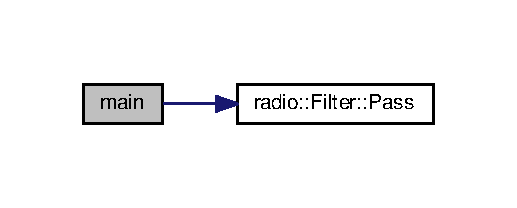
\includegraphics[width=248pt]{baseband__filter__test_8cpp_ae66f6b31b5ad750f1fe042a706a4e3d4_cgraph}
\end{center}
\end{figure}



\hypertarget{baseband__filter__test_8cpp_source}{\section{baseband\+\_\+filter\+\_\+test.\+cpp}
\label{baseband__filter__test_8cpp_source}\index{src/baseband\+\_\+filter\+\_\+test.\+cpp@{src/baseband\+\_\+filter\+\_\+test.\+cpp}}
}

\begin{DoxyCode}
00001 
00007 \textcolor{preprocessor}{#include <cstdio>}
00008 \textcolor{preprocessor}{#include <cstdlib>}
00009 \textcolor{preprocessor}{#include <iostream>}
00010 \textcolor{preprocessor}{#include <unistd.h>}
00011 
00012 \textcolor{preprocessor}{#include "\hyperlink{auxiliary_8hpp}{auxiliary.hpp}"}
00013 \textcolor{preprocessor}{#include "\hyperlink{definitions_8hpp}{definitions.hpp}"}
00014 \textcolor{preprocessor}{#include "\hyperlink{Filter_8hpp}{Filter.hpp}"}
00015 \textcolor{preprocessor}{#include "\hyperlink{fvectors_8hpp}{fvectors.hpp}"}
00016 \textcolor{preprocessor}{#include "\hyperlink{Sinusoid_8hpp}{Sinusoid.hpp}"}
00017 \textcolor{preprocessor}{#include "\hyperlink{zdomain_8hpp}{zdomain.hpp}"}
00018 
00019 \textcolor{keyword}{using namespace }\hyperlink{namespacestd}{std};
00020 \textcolor{keyword}{using namespace }\hyperlink{namespaceradio}{radio};
00021 
\hypertarget{baseband__filter__test_8cpp_source_l00025}{}\hyperlink{baseband__filter__test_8cpp_a0ddf1224851353fc92bfbff6f499fa97}{00025} \textcolor{keywordtype}{int} \hyperlink{baseband__filter__test_8cpp_a0ddf1224851353fc92bfbff6f499fa97}{main}(\textcolor{keywordtype}{int} argc, \textcolor{keywordtype}{char}* argv[]) \{
00026 
00027     \textcolor{comment}{// Constants}
00028     \textcolor{keyword}{const} \hyperlink{definitions_8hpp_a05f6b0ae8f6a6e135b0e290c25fe0e4e}{uint16} BUFFER\_SIZE = 48000;
00029 
00030     \textcolor{comment}{// Declare primative Variables}
00031     \hyperlink{definitions_8hpp_adde6aaee8457bee49c2a92621fe22b79}{uint8} i = 0;
00032     \hyperlink{definitions_8hpp_adde6aaee8457bee49c2a92621fe22b79}{uint8} size = 0;
00033     \hyperlink{definitions_8hpp_a05f6b0ae8f6a6e135b0e290c25fe0e4e}{uint16} delta = 250;
00034     \hyperlink{definitions_8hpp_aacdc525d6f7bddb3ae95d5c311bd06a1}{float32} dataBuffer[BUFFER\_SIZE];
00035     \hyperlink{definitions_8hpp_aacdc525d6f7bddb3ae95d5c311bd06a1}{float32} iqBuffer[2 * BUFFER\_SIZE];
00036 
00037     \textcolor{comment}{// create 1 sec of audio}
00038     \textcolor{keywordflow}{for}(\hyperlink{definitions_8hpp_a05f6b0ae8f6a6e135b0e290c25fe0e4e}{uint16} f = delta; f <= 3000; f += delta, i++) \{
00039         \hyperlink{classradio_1_1Sinusoid}{Sinusoid} sinusoid(f);
00040 
00041         \textcolor{keywordflow}{for}(\hyperlink{definitions_8hpp_a05f6b0ae8f6a6e135b0e290c25fe0e4e}{uint16} i = 0; i < BUFFER\_SIZE; i++) \{
00042             dataBuffer[i] += sinusoid.\hyperlink{classradio_1_1Sinusoid_aab44298ea1bd5cb175d5826243cf56f2}{next}();
00043         \}
00044     \}
00045 
00046     size = i;
00047     
00048     \textcolor{comment}{// adjust dataBuffer so values are between -1 and 1}
00049     \textcolor{keywordflow}{for}(\hyperlink{definitions_8hpp_a05f6b0ae8f6a6e135b0e290c25fe0e4e}{uint16} i = 0; i < BUFFER\_SIZE; i++) \{
00050         dataBuffer[i] /= size;
00051     \}
00052     
00053     \hyperlink{classradio_1_1Filter}{Filter} filter(dataBuffer, BUFFER\_SIZE, \hyperlink{namespaceradio_a9bd902e9216499953a5906de73dc1796}{F\_BASEBAND});
00054     filter.\hyperlink{classradio_1_1Filter_ad2793821801780809af385463bf8f197}{Pass}();
00055     \hyperlink{namespaceradio_a7166522e76ff88e8d482491b1b6e2275}{makeIQ}(dataBuffer, iqBuffer, BUFFER\_SIZE);
00056     \hyperlink{namespaceradio_ae4b2334c4366dcdf0311ad79d2067945}{to\_sint32}(iqBuffer, 2 * BUFFER\_SIZE);
00057 
00058     \textcolor{keywordflow}{while}(\textcolor{keyword}{true}) \{
00059         write(STDOUT\_FILENO, &iqBuffer, 2 * BUFFER\_SIZE * \textcolor{keyword}{sizeof}(\hyperlink{definitions_8hpp_a0573de65958b4fda3a0460ed417dafb8}{sint32}));
00060     \}
00061 \}
\end{DoxyCode}

\hypertarget{definitions_8hpp}{\section{src/definitions.hpp File Reference}
\label{definitions_8hpp}\index{src/definitions.\+hpp@{src/definitions.\+hpp}}
}


Contains declarations of system-\/independant (universal size) integers and float types, shortened type names for some commonly used types, and enumerations.  


{\ttfamily \#include $<$complex$>$}\\*
Include dependency graph for definitions.\+hpp\+:
\nopagebreak
\begin{figure}[H]
\begin{center}
\leavevmode
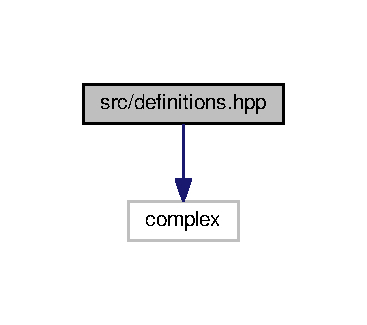
\includegraphics[width=176pt]{definitions_8hpp__incl}
\end{center}
\end{figure}
This graph shows which files directly or indirectly include this file\+:
\nopagebreak
\begin{figure}[H]
\begin{center}
\leavevmode
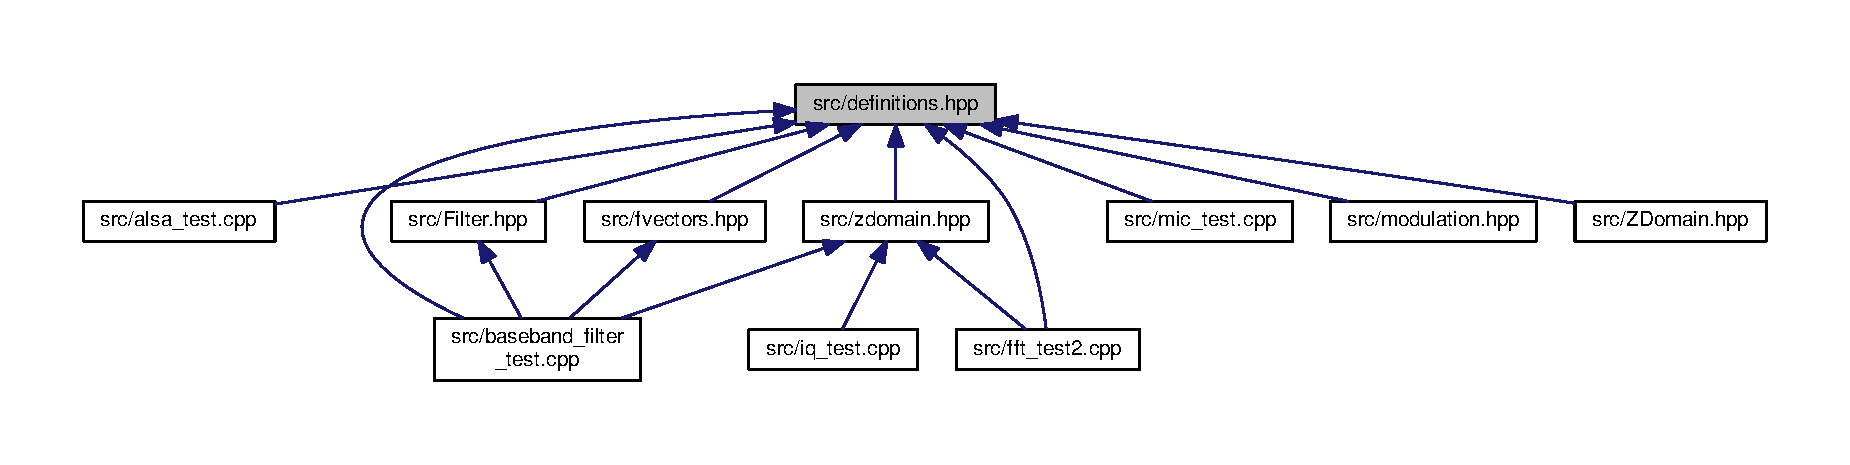
\includegraphics[width=350pt]{definitions_8hpp__dep__incl}
\end{center}
\end{figure}
\subsection*{Namespaces}
\begin{DoxyCompactItemize}
\item 
 \hyperlink{namespaceradio}{radio}
\end{DoxyCompactItemize}
\subsection*{Macros}
\begin{DoxyCompactItemize}
\item 
\#define \hyperlink{definitions_8hpp_a378181c29a641d58f55d647b5a9599f2}{E\+N\+U\+M}~signed char
\end{DoxyCompactItemize}
\subsection*{Typedefs}
\begin{DoxyCompactItemize}
\item 
typedef unsigned char \hyperlink{definitions_8hpp_a0c8186d9b9b7880309c27230bbb5e69d}{byte}
\item 
typedef unsigned char \hyperlink{definitions_8hpp_adde6aaee8457bee49c2a92621fe22b79}{uint8}
\item 
typedef signed char \hyperlink{definitions_8hpp_a1a6408291ee3cfd0760a61ac64084154}{sint8}
\item 
typedef unsigned short \hyperlink{definitions_8hpp_a05f6b0ae8f6a6e135b0e290c25fe0e4e}{uint16}
\item 
typedef signed short \hyperlink{definitions_8hpp_a74df79fde3c518e55b29ce6360a9c76e}{sint16}
\item 
typedef unsigned int \hyperlink{definitions_8hpp_a1134b580f8da4de94ca6b1de4d37975e}{uint32}
\item 
typedef signed int \hyperlink{definitions_8hpp_a0573de65958b4fda3a0460ed417dafb8}{sint32}
\item 
typedef unsigned long long \hyperlink{definitions_8hpp_a29940ae63ec06c9998bba873e25407ad}{uint64}
\item 
typedef signed long long \hyperlink{definitions_8hpp_ad91d7e42d1c1abce1d9eeacd54cc0497}{sint64}
\item 
typedef float \hyperlink{definitions_8hpp_aacdc525d6f7bddb3ae95d5c311bd06a1}{float32}
\item 
typedef double \hyperlink{definitions_8hpp_a232fad1b0d6dcc7c16aabde98b2e2a80}{float64}
\item 
typedef std\+::complex$<$ \hyperlink{definitions_8hpp_aacdc525d6f7bddb3ae95d5c311bd06a1}{float32} $>$ \hyperlink{definitions_8hpp_a960be6b6614c08090c16574dba10a421}{cfloat32}
\item 
typedef std\+::vector\\*
$<$ std\+::vector$<$ \hyperlink{definitions_8hpp_aacdc525d6f7bddb3ae95d5c311bd06a1}{float32} $>$ $>$ \hyperlink{definitions_8hpp_af19387f95516e2132a08cf60503f22a5}{fparams}
\end{DoxyCompactItemize}
\subsection*{Enumerations}
\begin{DoxyCompactItemize}
\item 
enum \hyperlink{namespaceradio_a90839d95c13fa21f45e9cd380e38f1f3}{radio\+::\+Age} \{ \hyperlink{namespaceradio_a90839d95c13fa21f45e9cd380e38f1f3afbe8ecd067dc1095175b7cdc7cecbb82}{radio\+::\+O\+L\+D}, 
\hyperlink{namespaceradio_a90839d95c13fa21f45e9cd380e38f1f3ac1a7d3b0b6d1c9639e94bdd8c8692686}{radio\+::\+N\+E\+W}
 \}
\item 
enum \hyperlink{namespaceradio_aa2a4fb91116a2b9a094776a29cce0dac}{radio\+::\+Fractional} \{ \hyperlink{namespaceradio_aa2a4fb91116a2b9a094776a29cce0daca7436a425f0fd0f72aa39de328f2bdd48}{radio\+::\+N\+U\+M}, 
\hyperlink{namespaceradio_aa2a4fb91116a2b9a094776a29cce0daca2fd2fe719e453d2bda50a402c0f49abe}{radio\+::\+D\+E\+N}
 \}
\end{DoxyCompactItemize}


\subsection{Detailed Description}
Contains declarations of system-\/independant (universal size) integers and float types, shortened type names for some commonly used types, and enumerations. 

\begin{DoxyAuthor}{Author}
Samuel Andrew Wisner, \href{mailto:awisner94@gmail.com}{\tt awisner94@gmail.\+com} 
\end{DoxyAuthor}


Definition in file \hyperlink{definitions_8hpp_source}{definitions.\+hpp}.



\subsection{Macro Definition Documentation}
\hypertarget{definitions_8hpp_a378181c29a641d58f55d647b5a9599f2}{\index{definitions.\+hpp@{definitions.\+hpp}!E\+N\+U\+M@{E\+N\+U\+M}}
\index{E\+N\+U\+M@{E\+N\+U\+M}!definitions.\+hpp@{definitions.\+hpp}}
\subsubsection[{E\+N\+U\+M}]{\setlength{\rightskip}{0pt plus 5cm}\#define E\+N\+U\+M~signed char}}\label{definitions_8hpp_a378181c29a641d58f55d647b5a9599f2}


Definition at line 14 of file definitions.\+hpp.



\subsection{Typedef Documentation}
\hypertarget{definitions_8hpp_a0c8186d9b9b7880309c27230bbb5e69d}{\index{definitions.\+hpp@{definitions.\+hpp}!byte@{byte}}
\index{byte@{byte}!definitions.\+hpp@{definitions.\+hpp}}
\subsubsection[{byte}]{\setlength{\rightskip}{0pt plus 5cm}typedef unsigned char {\bf byte}}}\label{definitions_8hpp_a0c8186d9b9b7880309c27230bbb5e69d}


Definition at line 16 of file definitions.\+hpp.

\hypertarget{definitions_8hpp_a960be6b6614c08090c16574dba10a421}{\index{definitions.\+hpp@{definitions.\+hpp}!cfloat32@{cfloat32}}
\index{cfloat32@{cfloat32}!definitions.\+hpp@{definitions.\+hpp}}
\subsubsection[{cfloat32}]{\setlength{\rightskip}{0pt plus 5cm}typedef std\+::complex$<${\bf float32}$>$ {\bf cfloat32}}}\label{definitions_8hpp_a960be6b6614c08090c16574dba10a421}
Defines a type for complex float32's. 

Definition at line 35 of file definitions.\+hpp.

\hypertarget{definitions_8hpp_aacdc525d6f7bddb3ae95d5c311bd06a1}{\index{definitions.\+hpp@{definitions.\+hpp}!float32@{float32}}
\index{float32@{float32}!definitions.\+hpp@{definitions.\+hpp}}
\subsubsection[{float32}]{\setlength{\rightskip}{0pt plus 5cm}typedef float {\bf float32}}}\label{definitions_8hpp_aacdc525d6f7bddb3ae95d5c311bd06a1}


Definition at line 29 of file definitions.\+hpp.

\hypertarget{definitions_8hpp_a232fad1b0d6dcc7c16aabde98b2e2a80}{\index{definitions.\+hpp@{definitions.\+hpp}!float64@{float64}}
\index{float64@{float64}!definitions.\+hpp@{definitions.\+hpp}}
\subsubsection[{float64}]{\setlength{\rightskip}{0pt plus 5cm}typedef double {\bf float64}}}\label{definitions_8hpp_a232fad1b0d6dcc7c16aabde98b2e2a80}


Definition at line 30 of file definitions.\+hpp.

\hypertarget{definitions_8hpp_af19387f95516e2132a08cf60503f22a5}{\index{definitions.\+hpp@{definitions.\+hpp}!fparams@{fparams}}
\index{fparams@{fparams}!definitions.\+hpp@{definitions.\+hpp}}
\subsubsection[{fparams}]{\setlength{\rightskip}{0pt plus 5cm}typedef std\+::vector$<$std\+::vector$<${\bf float32}$>$ $>$ {\bf fparams}}}\label{definitions_8hpp_af19387f95516e2132a08cf60503f22a5}
Defines a type for the filter coefficients. 

Definition at line 40 of file definitions.\+hpp.

\hypertarget{definitions_8hpp_a74df79fde3c518e55b29ce6360a9c76e}{\index{definitions.\+hpp@{definitions.\+hpp}!sint16@{sint16}}
\index{sint16@{sint16}!definitions.\+hpp@{definitions.\+hpp}}
\subsubsection[{sint16}]{\setlength{\rightskip}{0pt plus 5cm}typedef signed short {\bf sint16}}}\label{definitions_8hpp_a74df79fde3c518e55b29ce6360a9c76e}


Definition at line 21 of file definitions.\+hpp.

\hypertarget{definitions_8hpp_a0573de65958b4fda3a0460ed417dafb8}{\index{definitions.\+hpp@{definitions.\+hpp}!sint32@{sint32}}
\index{sint32@{sint32}!definitions.\+hpp@{definitions.\+hpp}}
\subsubsection[{sint32}]{\setlength{\rightskip}{0pt plus 5cm}typedef signed int {\bf sint32}}}\label{definitions_8hpp_a0573de65958b4fda3a0460ed417dafb8}


Definition at line 24 of file definitions.\+hpp.

\hypertarget{definitions_8hpp_ad91d7e42d1c1abce1d9eeacd54cc0497}{\index{definitions.\+hpp@{definitions.\+hpp}!sint64@{sint64}}
\index{sint64@{sint64}!definitions.\+hpp@{definitions.\+hpp}}
\subsubsection[{sint64}]{\setlength{\rightskip}{0pt plus 5cm}typedef signed long long {\bf sint64}}}\label{definitions_8hpp_ad91d7e42d1c1abce1d9eeacd54cc0497}


Definition at line 27 of file definitions.\+hpp.

\hypertarget{definitions_8hpp_a1a6408291ee3cfd0760a61ac64084154}{\index{definitions.\+hpp@{definitions.\+hpp}!sint8@{sint8}}
\index{sint8@{sint8}!definitions.\+hpp@{definitions.\+hpp}}
\subsubsection[{sint8}]{\setlength{\rightskip}{0pt plus 5cm}typedef signed char {\bf sint8}}}\label{definitions_8hpp_a1a6408291ee3cfd0760a61ac64084154}


Definition at line 18 of file definitions.\+hpp.

\hypertarget{definitions_8hpp_a05f6b0ae8f6a6e135b0e290c25fe0e4e}{\index{definitions.\+hpp@{definitions.\+hpp}!uint16@{uint16}}
\index{uint16@{uint16}!definitions.\+hpp@{definitions.\+hpp}}
\subsubsection[{uint16}]{\setlength{\rightskip}{0pt plus 5cm}typedef unsigned short {\bf uint16}}}\label{definitions_8hpp_a05f6b0ae8f6a6e135b0e290c25fe0e4e}


Definition at line 20 of file definitions.\+hpp.

\hypertarget{definitions_8hpp_a1134b580f8da4de94ca6b1de4d37975e}{\index{definitions.\+hpp@{definitions.\+hpp}!uint32@{uint32}}
\index{uint32@{uint32}!definitions.\+hpp@{definitions.\+hpp}}
\subsubsection[{uint32}]{\setlength{\rightskip}{0pt plus 5cm}typedef unsigned int {\bf uint32}}}\label{definitions_8hpp_a1134b580f8da4de94ca6b1de4d37975e}


Definition at line 23 of file definitions.\+hpp.

\hypertarget{definitions_8hpp_a29940ae63ec06c9998bba873e25407ad}{\index{definitions.\+hpp@{definitions.\+hpp}!uint64@{uint64}}
\index{uint64@{uint64}!definitions.\+hpp@{definitions.\+hpp}}
\subsubsection[{uint64}]{\setlength{\rightskip}{0pt plus 5cm}typedef unsigned long long {\bf uint64}}}\label{definitions_8hpp_a29940ae63ec06c9998bba873e25407ad}


Definition at line 26 of file definitions.\+hpp.

\hypertarget{definitions_8hpp_adde6aaee8457bee49c2a92621fe22b79}{\index{definitions.\+hpp@{definitions.\+hpp}!uint8@{uint8}}
\index{uint8@{uint8}!definitions.\+hpp@{definitions.\+hpp}}
\subsubsection[{uint8}]{\setlength{\rightskip}{0pt plus 5cm}typedef unsigned char {\bf uint8}}}\label{definitions_8hpp_adde6aaee8457bee49c2a92621fe22b79}


Definition at line 17 of file definitions.\+hpp.


\hypertarget{definitions_8hpp_source}{\section{definitions.\+hpp}
\label{definitions_8hpp_source}\index{src/definitions.\+hpp@{src/definitions.\+hpp}}
}

\begin{DoxyCode}
00001 
00009 \textcolor{preprocessor}{#ifndef definitions\_H}
00010 \textcolor{preprocessor}{#define definitions\_H}
00011 
00012 \textcolor{preprocessor}{#include <complex>}
00013 \textcolor{preprocessor}{#include <vector>}
00014 
\hypertarget{definitions_8hpp_source_l00018}{}\hyperlink{definitions_8hpp_a378181c29a641d58f55d647b5a9599f2}{00018} \textcolor{preprocessor}{#define ENUM signed char}
00019 
\hypertarget{definitions_8hpp_source_l00023}{}\hyperlink{definitions_8hpp_a8fe83ac76edc595f6b98cd4a4127aed5}{00023} \textcolor{preprocessor}{#define ERROR -1}
00024 
\hypertarget{definitions_8hpp_source_l00025}{}\hyperlink{definitions_8hpp_a0c8186d9b9b7880309c27230bbb5e69d}{00025} \textcolor{keyword}{typedef} \textcolor{keywordtype}{unsigned} \textcolor{keywordtype}{char} \hyperlink{definitions_8hpp_a0c8186d9b9b7880309c27230bbb5e69d}{byte};
\hypertarget{definitions_8hpp_source_l00026}{}\hyperlink{definitions_8hpp_adde6aaee8457bee49c2a92621fe22b79}{00026} \textcolor{keyword}{typedef} \textcolor{keywordtype}{unsigned} \textcolor{keywordtype}{char} \hyperlink{definitions_8hpp_adde6aaee8457bee49c2a92621fe22b79}{uint8};
\hypertarget{definitions_8hpp_source_l00027}{}\hyperlink{definitions_8hpp_a1a6408291ee3cfd0760a61ac64084154}{00027} \textcolor{keyword}{typedef} \textcolor{keywordtype}{signed} \textcolor{keywordtype}{char} \hyperlink{definitions_8hpp_a1a6408291ee3cfd0760a61ac64084154}{sint8};
00028 
\hypertarget{definitions_8hpp_source_l00029}{}\hyperlink{definitions_8hpp_a05f6b0ae8f6a6e135b0e290c25fe0e4e}{00029} \textcolor{keyword}{typedef} \textcolor{keywordtype}{unsigned} \textcolor{keywordtype}{short} \hyperlink{definitions_8hpp_a05f6b0ae8f6a6e135b0e290c25fe0e4e}{uint16};
\hypertarget{definitions_8hpp_source_l00030}{}\hyperlink{definitions_8hpp_a74df79fde3c518e55b29ce6360a9c76e}{00030} \textcolor{keyword}{typedef} \textcolor{keywordtype}{signed} \textcolor{keywordtype}{short} \hyperlink{definitions_8hpp_a74df79fde3c518e55b29ce6360a9c76e}{sint16};
00031 
\hypertarget{definitions_8hpp_source_l00032}{}\hyperlink{definitions_8hpp_a1134b580f8da4de94ca6b1de4d37975e}{00032} \textcolor{keyword}{typedef} \textcolor{keywordtype}{unsigned} \textcolor{keywordtype}{int} \hyperlink{definitions_8hpp_a1134b580f8da4de94ca6b1de4d37975e}{uint32};
\hypertarget{definitions_8hpp_source_l00033}{}\hyperlink{definitions_8hpp_a0573de65958b4fda3a0460ed417dafb8}{00033} \textcolor{keyword}{typedef} \textcolor{keywordtype}{signed} \textcolor{keywordtype}{int} \hyperlink{definitions_8hpp_a0573de65958b4fda3a0460ed417dafb8}{sint32};
00034 
\hypertarget{definitions_8hpp_source_l00035}{}\hyperlink{definitions_8hpp_a29940ae63ec06c9998bba873e25407ad}{00035} \textcolor{keyword}{typedef} \textcolor{keywordtype}{unsigned} \textcolor{keywordtype}{long} \textcolor{keywordtype}{long} \hyperlink{definitions_8hpp_a29940ae63ec06c9998bba873e25407ad}{uint64};
\hypertarget{definitions_8hpp_source_l00036}{}\hyperlink{definitions_8hpp_ad91d7e42d1c1abce1d9eeacd54cc0497}{00036} \textcolor{keyword}{typedef} \textcolor{keywordtype}{signed} \textcolor{keywordtype}{long} \textcolor{keywordtype}{long} \hyperlink{definitions_8hpp_ad91d7e42d1c1abce1d9eeacd54cc0497}{sint64};
00037 
\hypertarget{definitions_8hpp_source_l00038}{}\hyperlink{definitions_8hpp_aacdc525d6f7bddb3ae95d5c311bd06a1}{00038} \textcolor{keyword}{typedef} \textcolor{keywordtype}{float} \hyperlink{definitions_8hpp_aacdc525d6f7bddb3ae95d5c311bd06a1}{float32};
\hypertarget{definitions_8hpp_source_l00039}{}\hyperlink{definitions_8hpp_a232fad1b0d6dcc7c16aabde98b2e2a80}{00039} \textcolor{keyword}{typedef} \textcolor{keywordtype}{double} \hyperlink{definitions_8hpp_a232fad1b0d6dcc7c16aabde98b2e2a80}{float64};
00040 
\hypertarget{definitions_8hpp_source_l00044}{}\hyperlink{definitions_8hpp_a960be6b6614c08090c16574dba10a421}{00044} \textcolor{keyword}{typedef} std::complex<float32> \hyperlink{definitions_8hpp_a960be6b6614c08090c16574dba10a421}{cfloat32};
00045 
\hypertarget{definitions_8hpp_source_l00049}{}\hyperlink{definitions_8hpp_a7615684c2af56be5f302c5b367d71f6b}{00049} \textcolor{keyword}{typedef} std::vector<std::vector<float64>> \hyperlink{definitions_8hpp_a7615684c2af56be5f302c5b367d71f6b}{fparams};
00050 
00055 \textcolor{keyword}{namespace }\hyperlink{namespaceradio}{radio} \{
\hypertarget{definitions_8hpp_source_l00060}{}\hyperlink{namespaceradio_a90839d95c13fa21f45e9cd380e38f1f3afbe8ecd067dc1095175b7cdc7cecbb82}{00060}     \textcolor{keyword}{enum} \hyperlink{namespaceradio_a90839d95c13fa21f45e9cd380e38f1f3}{Age} \{ \hyperlink{namespaceradio_a90839d95c13fa21f45e9cd380e38f1f3afbe8ecd067dc1095175b7cdc7cecbb82}{OLD}, \hyperlink{namespaceradio_a90839d95c13fa21f45e9cd380e38f1f3ac1a7d3b0b6d1c9639e94bdd8c8692686}{NEW} \};
00061 
\hypertarget{definitions_8hpp_source_l00065}{}\hyperlink{namespaceradio_aa2a4fb91116a2b9a094776a29cce0daca7436a425f0fd0f72aa39de328f2bdd48}{00065}     \textcolor{keyword}{enum} \hyperlink{namespaceradio_aa2a4fb91116a2b9a094776a29cce0dac}{Fractional} \{ \hyperlink{namespaceradio_aa2a4fb91116a2b9a094776a29cce0daca7436a425f0fd0f72aa39de328f2bdd48}{NUM}, \hyperlink{namespaceradio_aa2a4fb91116a2b9a094776a29cce0daca2fd2fe719e453d2bda50a402c0f49abe}{DEN} \};
00066 
\hypertarget{definitions_8hpp_source_l00070}{}\hyperlink{namespaceradio_adf83fa57d52181b9779a376c3a98b4f5a145a49f0c5e95c6f59e51825a5a4817d}{00070}     \textcolor{keyword}{enum} \hyperlink{namespaceradio_adf83fa57d52181b9779a376c3a98b4f5}{Argument} \{ \hyperlink{namespaceradio_adf83fa57d52181b9779a376c3a98b4f5a47cc56722e29261caff496eb98ff3d88}{FREQ} = 1, \hyperlink{namespaceradio_adf83fa57d52181b9779a376c3a98b4f5a70b58e67bda4ad9bd46e010e1f090c7b}{MODE}, \hyperlink{namespaceradio_adf83fa57d52181b9779a376c3a98b4f5a145a49f0c5e95c6f59e51825a5a4817d}{PL\_TONE} \};
00071     
\hypertarget{definitions_8hpp_source_l00075}{}\hyperlink{namespaceradio_a46fb7299001138f28b7f69975c58399e}{00075}     \textcolor{keyword}{enum class} \hyperlink{namespaceradio_a46fb7299001138f28b7f69975c58399e}{ModulationType} \{
00076         \hyperlink{namespaceradio_a46fb7299001138f28b7f69975c58399eaf180dafbc98f54c6382ae29243cec902}{DSB\_LC}, \hyperlink{namespaceradio_a46fb7299001138f28b7f69975c58399ea92c257208ae8b0c6d88c80abcf15ec31}{DSB\_SC},
00077         \hyperlink{namespaceradio_a46fb7299001138f28b7f69975c58399ea9d8eca0470206cddb0dd0297717eb876}{USB\_FILTERED},
00078         \hyperlink{namespaceradio_a46fb7299001138f28b7f69975c58399ea1b14284e455bf5c311de662665312d13}{USB\_HILBERT},
00079         \hyperlink{namespaceradio_a46fb7299001138f28b7f69975c58399eaa6fd9ffa81c9d5e4a255b0c3b2336bd8}{LSB\_FILTERED},
00080         \hyperlink{namespaceradio_a46fb7299001138f28b7f69975c58399ea18f970daa5b5a8f72cbd45f7b49a6b6a}{LSB\_HILBERT},
00081         \hyperlink{namespaceradio_a46fb7299001138f28b7f69975c58399ea7b4b1e7876b8d9de5b77b9264fbe556a}{FM\_NARROW},
00082         \hyperlink{namespaceradio_a46fb7299001138f28b7f69975c58399eafabee3b32b363b14950cb5f5b61e998c}{FM\_WIDE}
00083     \};
00084 \}
00085 
00086 \textcolor{preprocessor}{#endif}
00087 
00088 \textcolor{comment}{// Doxygen descriptions for non-code files}
00089 
\end{DoxyCode}

\hypertarget{fft__test_8cpp}{\section{src/fft\+\_\+test.cpp File Reference}
\label{fft__test_8cpp}\index{src/fft\+\_\+test.\+cpp@{src/fft\+\_\+test.\+cpp}}
}


Tests F\+F\+T, I\+F\+F\+T, and Hilbert implementations.  


{\ttfamily \#include $<$complex$>$}\\*
{\ttfamily \#include $<$functional$>$}\\*
{\ttfamily \#include $<$iostream$>$}\\*
{\ttfamily \#include $<$valarray$>$}\\*
Include dependency graph for fft\+\_\+test.\+cpp\+:
\nopagebreak
\begin{figure}[H]
\begin{center}
\leavevmode
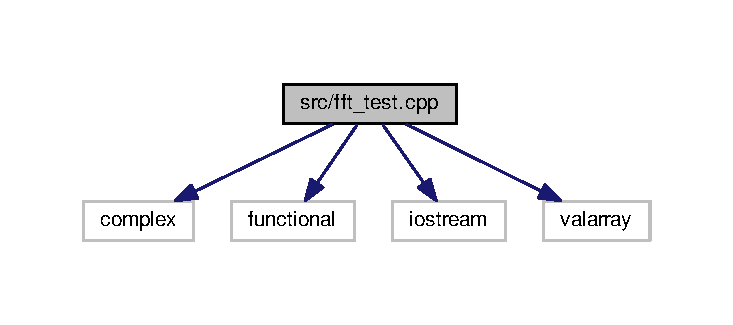
\includegraphics[width=350pt]{fft__test_8cpp__incl}
\end{center}
\end{figure}
\subsection*{Typedefs}
\begin{DoxyCompactItemize}
\item 
typedef std\+::valarray\\*
$<$ std\+::complex$<$ double $>$ $>$ \hyperlink{fft__test_8cpp_ac43c8a7b2d97f3ccbd6f7a48beaa472c}{C\+Array}
\end{DoxyCompactItemize}
\subsection*{Functions}
\begin{DoxyCompactItemize}
\item 
void \hyperlink{fft__test_8cpp_a22051cd252d576aec530227d32d95bdd}{fft} (\hyperlink{fft__test_8cpp_ac43c8a7b2d97f3ccbd6f7a48beaa472c}{C\+Array} \&x)
\item 
void \hyperlink{fft__test_8cpp_a6234aee8acb83780e803805365617f36}{ifft} (\hyperlink{fft__test_8cpp_ac43c8a7b2d97f3ccbd6f7a48beaa472c}{C\+Array} \&x)
\item 
std\+::complex$<$ double $>$ \hyperlink{fft__test_8cpp_adc49b5a69e64611f421bbefee39a4d15}{hilbert} (std\+::complex$<$ double $>$ n)
\item 
int \hyperlink{fft__test_8cpp_ae66f6b31b5ad750f1fe042a706a4e3d4}{main} ()
\end{DoxyCompactItemize}
\subsection*{Variables}
\begin{DoxyCompactItemize}
\item 
const double \hyperlink{fft__test_8cpp_a952eac791b596a61bba0a133a3bb439f}{P\+I} = 3.\+141592653589793238460
\end{DoxyCompactItemize}


\subsection{Detailed Description}
Tests F\+F\+T, I\+F\+F\+T, and Hilbert implementations. 

\begin{DoxyAuthor}{Author}
Samuel Andrew Wisner, \href{mailto:awisner94@gmail.com}{\tt awisner94@gmail.\+com} 
\end{DoxyAuthor}


Definition in file \hyperlink{fft__test_8cpp_source}{fft\+\_\+test.\+cpp}.



\subsection{Typedef Documentation}
\hypertarget{fft__test_8cpp_ac43c8a7b2d97f3ccbd6f7a48beaa472c}{\index{fft\+\_\+test.\+cpp@{fft\+\_\+test.\+cpp}!C\+Array@{C\+Array}}
\index{C\+Array@{C\+Array}!fft\+\_\+test.\+cpp@{fft\+\_\+test.\+cpp}}
\subsubsection[{C\+Array}]{\setlength{\rightskip}{0pt plus 5cm}typedef std\+::valarray$<$std\+::complex$<$double$>$ $>$ {\bf C\+Array}}}\label{fft__test_8cpp_ac43c8a7b2d97f3ccbd6f7a48beaa472c}


Definition at line \hyperlink{fft__test_8cpp_source_l00014}{14} of file \hyperlink{fft__test_8cpp_source}{fft\+\_\+test.\+cpp}.



\subsection{Function Documentation}
\hypertarget{fft__test_8cpp_a22051cd252d576aec530227d32d95bdd}{\index{fft\+\_\+test.\+cpp@{fft\+\_\+test.\+cpp}!fft@{fft}}
\index{fft@{fft}!fft\+\_\+test.\+cpp@{fft\+\_\+test.\+cpp}}
\subsubsection[{fft}]{\setlength{\rightskip}{0pt plus 5cm}void fft (
\begin{DoxyParamCaption}
\item[{{\bf C\+Array} \&}]{x}
\end{DoxyParamCaption}
)}}\label{fft__test_8cpp_a22051cd252d576aec530227d32d95bdd}
This code was taken from \href{http://rosettacode.org/wiki/Fast_Fourier_transform#C.2B.2B}{\tt http\+://rosettacode.\+org/wiki/\+Fast\+\_\+\+Fourier\+\_\+transform\#\+C.\+2\+B.\+2\+B}. 

Definition at line \hyperlink{fft__test_8cpp_source_l00023}{23} of file \hyperlink{fft__test_8cpp_source}{fft\+\_\+test.\+cpp}.


\begin{DoxyCode}
00024 \{
00025     \textcolor{comment}{// DFT}
00026     \textcolor{keywordtype}{unsigned} \textcolor{keywordtype}{int} N = x.size(), k = N, n;
00027     \textcolor{keywordtype}{double} thetaT = 3.14159265358979323846264338328L / N;
00028     std::complex<double> phiT(cos(thetaT), sin(thetaT)), T;
00029     \textcolor{keywordflow}{while} (k > 1)
00030     \{
00031         n = k;
00032         k >>= 1;
00033         phiT = phiT * phiT;
00034         T = 1.0L;
00035         \textcolor{keywordflow}{for} (\textcolor{keywordtype}{unsigned} \textcolor{keywordtype}{int} l = 0; l < k; l++)
00036         \{
00037             \textcolor{keywordflow}{for} (\textcolor{keywordtype}{unsigned} \textcolor{keywordtype}{int} a = l; a < N; a += n)
00038             \{
00039                 \textcolor{keywordtype}{unsigned} \textcolor{keywordtype}{int} b = a + k;
00040                 std::complex<double> t = x[a] - x[b];
00041                 x[a] += x[b];
00042                 x[b] = t * T;
00043             \}
00044             T *= phiT;
00045         \}
00046     \}
00047     \textcolor{comment}{// Decimate}
00048     \textcolor{keywordtype}{unsigned} \textcolor{keywordtype}{int} m = (\textcolor{keywordtype}{unsigned} int)log2(N);
00049     \textcolor{keywordflow}{for} (\textcolor{keywordtype}{unsigned} \textcolor{keywordtype}{int} a = 0; a < N; a++)
00050     \{
00051         \textcolor{keywordtype}{unsigned} \textcolor{keywordtype}{int} b = a;
00052         \textcolor{comment}{// Reverse bits}
00053         b = (((b & 0xaaaaaaaa) >> 1) | ((b & 0x55555555) << 1));
00054         b = (((b & 0xcccccccc) >> 2) | ((b & 0x33333333) << 2));
00055         b = (((b & 0xf0f0f0f0) >> 4) | ((b & 0x0f0f0f0f) << 4));
00056         b = (((b & 0xff00ff00) >> 8) | ((b & 0x00ff00ff) << 8));
00057         b = ((b >> 16) | (b << 16)) >> (32 - m);
00058         \textcolor{keywordflow}{if} (b > a)
00059         \{
00060             std::complex<double> t = x[a];
00061             x[a] = x[b];
00062             x[b] = t;
00063         \}
00064     \}
00066     \textcolor{comment}{//std::complex<double> f = 1.0 / sqrt(N);}
00067     \textcolor{comment}{//for (unsigned int i = 0; i < N; i++)}
00068     \textcolor{comment}{//  x[i] *= f;}
00069 \}
\end{DoxyCode}


Here is the caller graph for this function\+:
\nopagebreak
\begin{figure}[H]
\begin{center}
\leavevmode
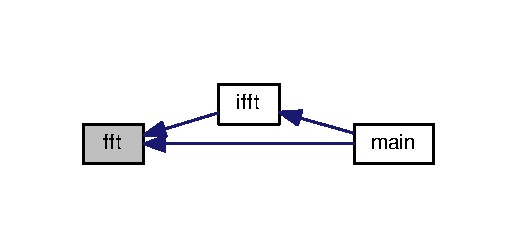
\includegraphics[width=248pt]{fft__test_8cpp_a22051cd252d576aec530227d32d95bdd_icgraph}
\end{center}
\end{figure}


\hypertarget{fft__test_8cpp_adc49b5a69e64611f421bbefee39a4d15}{\index{fft\+\_\+test.\+cpp@{fft\+\_\+test.\+cpp}!hilbert@{hilbert}}
\index{hilbert@{hilbert}!fft\+\_\+test.\+cpp@{fft\+\_\+test.\+cpp}}
\subsubsection[{hilbert}]{\setlength{\rightskip}{0pt plus 5cm}std\+::complex$<$double$>$ hilbert (
\begin{DoxyParamCaption}
\item[{std\+::complex$<$ double $>$}]{n}
\end{DoxyParamCaption}
)}}\label{fft__test_8cpp_adc49b5a69e64611f421bbefee39a4d15}


Definition at line \hyperlink{fft__test_8cpp_source_l00087}{87} of file \hyperlink{fft__test_8cpp_source}{fft\+\_\+test.\+cpp}.


\begin{DoxyCode}
00087                                                  \{
00088     \textcolor{keywordflow}{return} std::complex<double>(-2 * n.imag(), 0);
00089 \}
\end{DoxyCode}


Here is the caller graph for this function\+:
\nopagebreak
\begin{figure}[H]
\begin{center}
\leavevmode
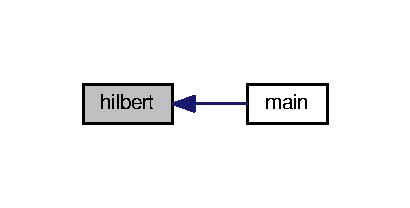
\includegraphics[width=197pt]{fft__test_8cpp_adc49b5a69e64611f421bbefee39a4d15_icgraph}
\end{center}
\end{figure}


\hypertarget{fft__test_8cpp_a6234aee8acb83780e803805365617f36}{\index{fft\+\_\+test.\+cpp@{fft\+\_\+test.\+cpp}!ifft@{ifft}}
\index{ifft@{ifft}!fft\+\_\+test.\+cpp@{fft\+\_\+test.\+cpp}}
\subsubsection[{ifft}]{\setlength{\rightskip}{0pt plus 5cm}void ifft (
\begin{DoxyParamCaption}
\item[{{\bf C\+Array} \&}]{x}
\end{DoxyParamCaption}
)}}\label{fft__test_8cpp_a6234aee8acb83780e803805365617f36}


Definition at line \hyperlink{fft__test_8cpp_source_l00072}{72} of file \hyperlink{fft__test_8cpp_source}{fft\+\_\+test.\+cpp}.


\begin{DoxyCode}
00073 \{
00074     \textcolor{comment}{// conjugate the complex numbers}
00075     x = x.apply(std::conj);
00076 
00077     \textcolor{comment}{// forward fft}
00078     \hyperlink{fft__test_8cpp_a22051cd252d576aec530227d32d95bdd}{fft}( x );
00079 
00080     \textcolor{comment}{// conjugate the complex numbers again}
00081     x = x.apply(std::conj);
00082 
00083     \textcolor{comment}{// scale the numbers}
00084     x /= x.size();
00085 \}
\end{DoxyCode}


Here is the call graph for this function\+:
\nopagebreak
\begin{figure}[H]
\begin{center}
\leavevmode
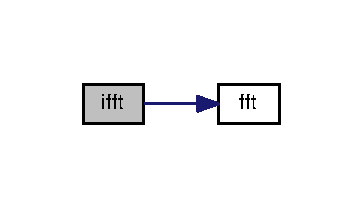
\includegraphics[width=174pt]{fft__test_8cpp_a6234aee8acb83780e803805365617f36_cgraph}
\end{center}
\end{figure}




Here is the caller graph for this function\+:
\nopagebreak
\begin{figure}[H]
\begin{center}
\leavevmode
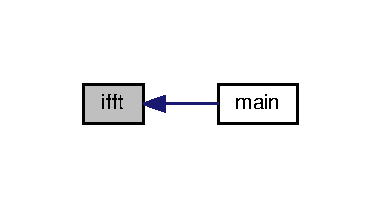
\includegraphics[width=183pt]{fft__test_8cpp_a6234aee8acb83780e803805365617f36_icgraph}
\end{center}
\end{figure}


\hypertarget{fft__test_8cpp_ae66f6b31b5ad750f1fe042a706a4e3d4}{\index{fft\+\_\+test.\+cpp@{fft\+\_\+test.\+cpp}!main@{main}}
\index{main@{main}!fft\+\_\+test.\+cpp@{fft\+\_\+test.\+cpp}}
\subsubsection[{main}]{\setlength{\rightskip}{0pt plus 5cm}int main (
\begin{DoxyParamCaption}
{}
\end{DoxyParamCaption}
)}}\label{fft__test_8cpp_ae66f6b31b5ad750f1fe042a706a4e3d4}


Definition at line \hyperlink{fft__test_8cpp_source_l00091}{91} of file \hyperlink{fft__test_8cpp_source}{fft\+\_\+test.\+cpp}.


\begin{DoxyCode}
00092 \{
00093     \textcolor{keyword}{const} std::complex<double> test[] = \{ 1,2,3,4,5,6,7,8,9,10,11,12,13,14,15,16 \};
00094     \hyperlink{fft__test_8cpp_ac43c8a7b2d97f3ccbd6f7a48beaa472c}{CArray} data(test, 16);
00095 
00096     \textcolor{comment}{// forward fft}
00097     \hyperlink{fft__test_8cpp_a22051cd252d576aec530227d32d95bdd}{fft}(data);
00098 
00099     std::cout << \textcolor{stringliteral}{"fft"} << std::endl;
00100     \textcolor{keywordflow}{for} (\textcolor{keywordtype}{int} i = 0; i < 16; ++i)
00101     \{
00102     \textcolor{comment}{//  std::cout << data[i] << std::endl;}
00103     \}
00104 
00105     \textcolor{keywordflow}{for}(\textcolor{keywordtype}{int} i = 8; i < 16; i++) \{
00106         data[i] = 0;
00107     \}
00108 
00109     \textcolor{comment}{// inverse fft}
00110     \hyperlink{fft__test_8cpp_a6234aee8acb83780e803805365617f36}{ifft}(data);
00111     std::cout << std::endl << \textcolor{stringliteral}{"ifft"} << std::endl;
00112 
00113     \textcolor{keywordflow}{for} (\textcolor{keywordtype}{int} i = 0; i < 16; ++i)
00114     \{
00115     \textcolor{comment}{//  std::cout << data[i] << std::endl;}
00116     \}
00117 
00118     data = data.apply(\hyperlink{fft__test_8cpp_adc49b5a69e64611f421bbefee39a4d15}{hilbert});
00119 
00120     std::cout << std::endl;
00121 
00122     \textcolor{keywordflow}{for}(\textcolor{keywordtype}{int} i = 0; i < 16; i++) \{
00123         std::cout << data[i].real() << std::endl;
00124     \}
00125 
00126     \textcolor{keywordflow}{return} 0;
00127 \}
\end{DoxyCode}


Here is the call graph for this function\+:
\nopagebreak
\begin{figure}[H]
\begin{center}
\leavevmode
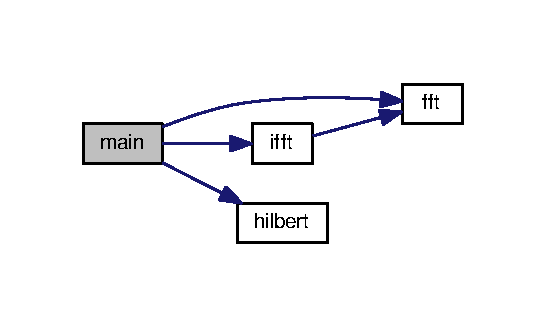
\includegraphics[width=262pt]{fft__test_8cpp_ae66f6b31b5ad750f1fe042a706a4e3d4_cgraph}
\end{center}
\end{figure}




\subsection{Variable Documentation}
\hypertarget{fft__test_8cpp_a952eac791b596a61bba0a133a3bb439f}{\index{fft\+\_\+test.\+cpp@{fft\+\_\+test.\+cpp}!P\+I@{P\+I}}
\index{P\+I@{P\+I}!fft\+\_\+test.\+cpp@{fft\+\_\+test.\+cpp}}
\subsubsection[{P\+I}]{\setlength{\rightskip}{0pt plus 5cm}const double P\+I = 3.\+141592653589793238460}}\label{fft__test_8cpp_a952eac791b596a61bba0a133a3bb439f}


Definition at line \hyperlink{fft__test_8cpp_source_l00012}{12} of file \hyperlink{fft__test_8cpp_source}{fft\+\_\+test.\+cpp}.


\hypertarget{fft__test_8cpp_source}{\section{fft\+\_\+test.\+cpp}
\label{fft__test_8cpp_source}\index{src/fft\+\_\+test.\+cpp@{src/fft\+\_\+test.\+cpp}}
}

\begin{DoxyCode}
00001 
00007 \textcolor{preprocessor}{#include <complex>}
00008 \textcolor{preprocessor}{#include <functional>}
00009 \textcolor{preprocessor}{#include <iostream>}
00010 \textcolor{preprocessor}{#include <valarray>}
00011 
\hypertarget{fft__test_8cpp_source_l00012}{}\hyperlink{fft__test_8cpp_a952eac791b596a61bba0a133a3bb439f}{00012} \textcolor{keyword}{const} \textcolor{keywordtype}{double} \hyperlink{fft__test_8cpp_a952eac791b596a61bba0a133a3bb439f}{PI} = 3.141592653589793238460;
00013 
\hypertarget{fft__test_8cpp_source_l00014}{}\hyperlink{fft__test_8cpp_ac43c8a7b2d97f3ccbd6f7a48beaa472c}{00014} \textcolor{keyword}{typedef} std::valarray<std::complex<double>> \hyperlink{fft__test_8cpp_ac43c8a7b2d97f3ccbd6f7a48beaa472c}{CArray};
00015 
00021 \textcolor{comment}{// Cooley-Tukey FFT (in-place, breadth-first, decimation-in-frequency)}
00022 \textcolor{comment}{// Better optimized but less intuitive}
\hypertarget{fft__test_8cpp_source_l00023}{}\hyperlink{fft__test_8cpp_a22051cd252d576aec530227d32d95bdd}{00023} \textcolor{keywordtype}{void} \hyperlink{fft__test_8cpp_a22051cd252d576aec530227d32d95bdd}{fft}(\hyperlink{fft__test_8cpp_ac43c8a7b2d97f3ccbd6f7a48beaa472c}{CArray} &x)
00024 \{
00025     \textcolor{comment}{// DFT}
00026     \textcolor{keywordtype}{unsigned} \textcolor{keywordtype}{int} N = x.size(), k = N, n;
00027     \textcolor{keywordtype}{double} thetaT = 3.14159265358979323846264338328L / N;
00028     std::complex<double> phiT(cos(thetaT), sin(thetaT)), T;
00029     \textcolor{keywordflow}{while} (k > 1)
00030     \{
00031         n = k;
00032         k >>= 1;
00033         phiT = phiT * phiT;
00034         T = 1.0L;
00035         \textcolor{keywordflow}{for} (\textcolor{keywordtype}{unsigned} \textcolor{keywordtype}{int} l = 0; l < k; l++)
00036         \{
00037             \textcolor{keywordflow}{for} (\textcolor{keywordtype}{unsigned} \textcolor{keywordtype}{int} a = l; a < N; a += n)
00038             \{
00039                 \textcolor{keywordtype}{unsigned} \textcolor{keywordtype}{int} b = a + k;
00040                 std::complex<double> t = x[a] - x[b];
00041                 x[a] += x[b];
00042                 x[b] = t * T;
00043             \}
00044             T *= phiT;
00045         \}
00046     \}
00047     \textcolor{comment}{// Decimate}
00048     \textcolor{keywordtype}{unsigned} \textcolor{keywordtype}{int} m = (\textcolor{keywordtype}{unsigned} int)log2(N);
00049     \textcolor{keywordflow}{for} (\textcolor{keywordtype}{unsigned} \textcolor{keywordtype}{int} a = 0; a < N; a++)
00050     \{
00051         \textcolor{keywordtype}{unsigned} \textcolor{keywordtype}{int} b = a;
00052         \textcolor{comment}{// Reverse bits}
00053         b = (((b & 0xaaaaaaaa) >> 1) | ((b & 0x55555555) << 1));
00054         b = (((b & 0xcccccccc) >> 2) | ((b & 0x33333333) << 2));
00055         b = (((b & 0xf0f0f0f0) >> 4) | ((b & 0x0f0f0f0f) << 4));
00056         b = (((b & 0xff00ff00) >> 8) | ((b & 0x00ff00ff) << 8));
00057         b = ((b >> 16) | (b << 16)) >> (32 - m);
00058         \textcolor{keywordflow}{if} (b > a)
00059         \{
00060             std::complex<double> t = x[a];
00061             x[a] = x[b];
00062             x[b] = t;
00063         \}
00064     \}
00066     \textcolor{comment}{//std::complex<double> f = 1.0 / sqrt(N);}
00067     \textcolor{comment}{//for (unsigned int i = 0; i < N; i++)}
00068     \textcolor{comment}{//  x[i] *= f;}
00069 \}
00070 
00071 \textcolor{comment}{// inverse fft (in-place)}
\hypertarget{fft__test_8cpp_source_l00072}{}\hyperlink{fft__test_8cpp_a6234aee8acb83780e803805365617f36}{00072} \textcolor{keywordtype}{void} \hyperlink{fft__test_8cpp_a6234aee8acb83780e803805365617f36}{ifft}(\hyperlink{fft__test_8cpp_ac43c8a7b2d97f3ccbd6f7a48beaa472c}{CArray}& x)
00073 \{
00074     \textcolor{comment}{// conjugate the complex numbers}
00075     x = x.apply(std::conj);
00076 
00077     \textcolor{comment}{// forward fft}
00078     \hyperlink{fft__test_8cpp_a22051cd252d576aec530227d32d95bdd}{fft}( x );
00079 
00080     \textcolor{comment}{// conjugate the complex numbers again}
00081     x = x.apply(std::conj);
00082 
00083     \textcolor{comment}{// scale the numbers}
00084     x /= x.size();
00085 \}
00086 
\hypertarget{fft__test_8cpp_source_l00087}{}\hyperlink{fft__test_8cpp_adc49b5a69e64611f421bbefee39a4d15}{00087} std::complex<double> \hyperlink{fft__test_8cpp_adc49b5a69e64611f421bbefee39a4d15}{hilbert}(std::complex<double> n) \{
00088     \textcolor{keywordflow}{return} std::complex<double>(-2 * n.imag(), 0);
00089 \}
00090 
\hypertarget{fft__test_8cpp_source_l00091}{}\hyperlink{fft__test_8cpp_ae66f6b31b5ad750f1fe042a706a4e3d4}{00091} \textcolor{keywordtype}{int} \hyperlink{fft__test_8cpp_ae66f6b31b5ad750f1fe042a706a4e3d4}{main}()
00092 \{
00093     \textcolor{keyword}{const} std::complex<double> test[] = \{ 1,2,3,4,5,6,7,8,9,10,11,12,13,14,15,16 \};
00094     \hyperlink{fft__test_8cpp_ac43c8a7b2d97f3ccbd6f7a48beaa472c}{CArray} data(test, 16);
00095 
00096     \textcolor{comment}{// forward fft}
00097     \hyperlink{fft__test_8cpp_a22051cd252d576aec530227d32d95bdd}{fft}(data);
00098 
00099     std::cout << \textcolor{stringliteral}{"fft"} << std::endl;
00100     \textcolor{keywordflow}{for} (\textcolor{keywordtype}{int} i = 0; i < 16; ++i)
00101     \{
00102     \textcolor{comment}{//  std::cout << data[i] << std::endl;}
00103     \}
00104 
00105     \textcolor{keywordflow}{for}(\textcolor{keywordtype}{int} i = 8; i < 16; i++) \{
00106         data[i] = 0;
00107     \}
00108 
00109     \textcolor{comment}{// inverse fft}
00110     \hyperlink{fft__test_8cpp_a6234aee8acb83780e803805365617f36}{ifft}(data);
00111     std::cout << std::endl << \textcolor{stringliteral}{"ifft"} << std::endl;
00112 
00113     \textcolor{keywordflow}{for} (\textcolor{keywordtype}{int} i = 0; i < 16; ++i)
00114     \{
00115     \textcolor{comment}{//  std::cout << data[i] << std::endl;}
00116     \}
00117 
00118     data = data.apply(\hyperlink{fft__test_8cpp_adc49b5a69e64611f421bbefee39a4d15}{hilbert});
00119 
00120     std::cout << std::endl;
00121 
00122     \textcolor{keywordflow}{for}(\textcolor{keywordtype}{int} i = 0; i < 16; i++) \{
00123         std::cout << data[i].real() << std::endl;
00124     \}
00125 
00126     \textcolor{keywordflow}{return} 0;
00127 \}
\end{DoxyCode}

\hypertarget{fft__test2_8cpp}{\section{src/fft\+\_\+test2.cpp File Reference}
\label{fft__test2_8cpp}\index{src/fft\+\_\+test2.\+cpp@{src/fft\+\_\+test2.\+cpp}}
}


Tests F\+F\+T, I\+F\+F\+T, and Hilbert implementations in \hyperlink{zdomain_8hpp}{zdomain.\+hpp}.  


{\ttfamily \#include $<$complex$>$}\\*
{\ttfamily \#include $<$iostream$>$}\\*
{\ttfamily \#include \char`\"{}definitions.\+hpp\char`\"{}}\\*
{\ttfamily \#include \char`\"{}zdomain.\+hpp\char`\"{}}\\*
Include dependency graph for fft\+\_\+test2.\+cpp\+:
\nopagebreak
\begin{figure}[H]
\begin{center}
\leavevmode
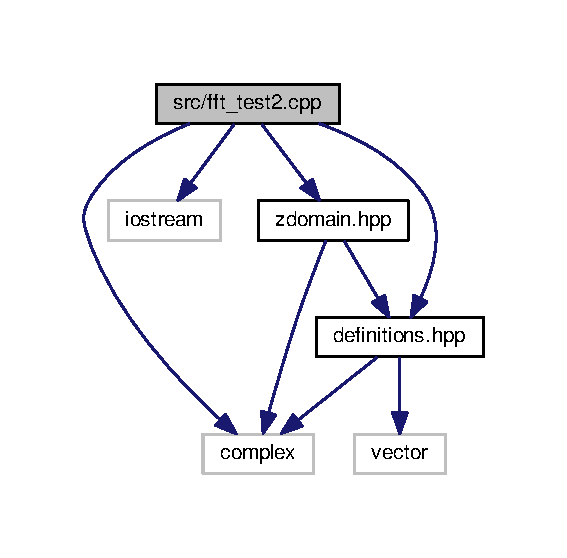
\includegraphics[width=272pt]{fft__test2_8cpp__incl}
\end{center}
\end{figure}
\subsection*{Functions}
\begin{DoxyCompactItemize}
\item 
int \hyperlink{fft__test2_8cpp_ae66f6b31b5ad750f1fe042a706a4e3d4}{main} ()
\end{DoxyCompactItemize}


\subsection{Detailed Description}
Tests F\+F\+T, I\+F\+F\+T, and Hilbert implementations in \hyperlink{zdomain_8hpp}{zdomain.\+hpp}. 

\begin{DoxyAuthor}{Author}
Samuel Andrew Wisner, \href{mailto:awisner94@gmail.com}{\tt awisner94@gmail.\+com} 
\end{DoxyAuthor}


Definition in file \hyperlink{fft__test2_8cpp_source}{fft\+\_\+test2.\+cpp}.



\subsection{Function Documentation}
\hypertarget{fft__test2_8cpp_ae66f6b31b5ad750f1fe042a706a4e3d4}{\index{fft\+\_\+test2.\+cpp@{fft\+\_\+test2.\+cpp}!main@{main}}
\index{main@{main}!fft\+\_\+test2.\+cpp@{fft\+\_\+test2.\+cpp}}
\subsubsection[{main}]{\setlength{\rightskip}{0pt plus 5cm}int main (
\begin{DoxyParamCaption}
{}
\end{DoxyParamCaption}
)}}\label{fft__test2_8cpp_ae66f6b31b5ad750f1fe042a706a4e3d4}
This program tests the \hyperlink{fft__test_8cpp_a22051cd252d576aec530227d32d95bdd}{fft()}, \hyperlink{fft__test_8cpp_a6234aee8acb83780e803805365617f36}{ifft()}, and \hyperlink{fft__test_8cpp_adc49b5a69e64611f421bbefee39a4d15}{hilbert()} functions in the \hyperlink{zdomain_8hpp}{zdomain.\+hpp} file.

This code is based on code from \href{http://rosettacode.org/wiki/Fast_Fourier_transform#C.2B.2B}{\tt http\+://rosettacode.\+org/wiki/\+Fast\+\_\+\+Fourier\+\_\+transform\#\+C.\+2\+B.\+2\+B}. 

Definition at line \hyperlink{fft__test2_8cpp_source_l00022}{22} of file \hyperlink{fft__test2_8cpp_source}{fft\+\_\+test2.\+cpp}.


\begin{DoxyCode}
00023 \{
00024     std::complex<float32> test[] = \{ 1,2,3,4,5,6,7,8,9,10,11,12,13,14,15,16 \};
00025     \hyperlink{definitions_8hpp_aacdc525d6f7bddb3ae95d5c311bd06a1}{float32} ftest[16];   
00026     \hyperlink{definitions_8hpp_aacdc525d6f7bddb3ae95d5c311bd06a1}{float32} dest[16];
00027 
00028     \textcolor{keywordflow}{for}(\textcolor{keywordtype}{int} i = 0; i < 16; i++) \{
00029         ftest[i] = test[i].real();
00030     \}
00031 
00032     \textcolor{comment}{// forward fft}
00033     \hyperlink{fft__test_8cpp_a22051cd252d576aec530227d32d95bdd}{fft}(test, 16);
00034 
00035     std::cout << \textcolor{stringliteral}{"fft"} << std::endl;
00036 
00037     \textcolor{keywordflow}{for} (\textcolor{keywordtype}{int} i = 0; i < 16; ++i)
00038     \{
00039     \textcolor{comment}{//  std::cout << test[i] << std::endl;}
00040     \}
00041 
00042     \textcolor{comment}{// inverse fft}
00043     \hyperlink{fft__test_8cpp_a6234aee8acb83780e803805365617f36}{ifft}(test, 16);
00044     std::cout << std::endl << \textcolor{stringliteral}{"ifft"} << std::endl;
00045 
00046     \textcolor{keywordflow}{for} (\textcolor{keywordtype}{int} i = 0; i < 16; ++i)
00047     \{
00048         std::cout << test[i] << std::endl;
00049     \}
00050 
00051     \hyperlink{fft__test_8cpp_adc49b5a69e64611f421bbefee39a4d15}{hilbert}(ftest, dest, 16);
00052     std::cout << std::endl << \textcolor{stringliteral}{"hilbert"} << std::endl;
00053 
00054     \textcolor{keywordflow}{for}(\textcolor{keywordtype}{int} i = 0; i < 16; i++) \{
00055         std::cout << dest[i] << std::endl;
00056     \}
00057 
00058     \textcolor{keywordflow}{return} 0;
00059 \}
\end{DoxyCode}


Here is the call graph for this function\+:
\nopagebreak
\begin{figure}[H]
\begin{center}
\leavevmode
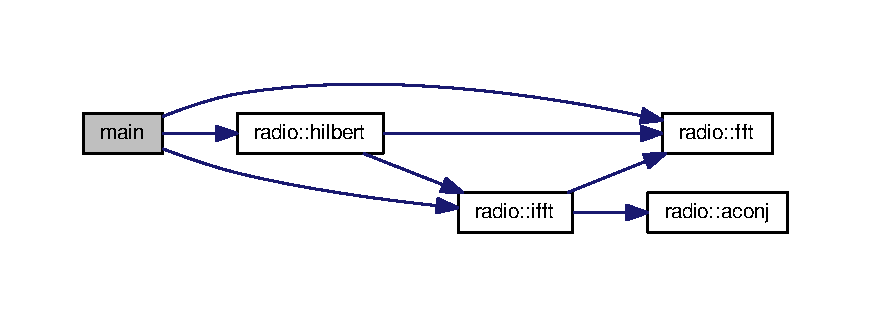
\includegraphics[width=350pt]{fft__test2_8cpp_ae66f6b31b5ad750f1fe042a706a4e3d4_cgraph}
\end{center}
\end{figure}



\hypertarget{fft__test2_8cpp_source}{\section{fft\+\_\+test2.\+cpp}
\label{fft__test2_8cpp_source}\index{src/fft\+\_\+test2.\+cpp@{src/fft\+\_\+test2.\+cpp}}
}

\begin{DoxyCode}
00001 
00007 \textcolor{preprocessor}{#include <complex>}
00008 \textcolor{preprocessor}{#include <iostream>}
00009 
00010 \textcolor{preprocessor}{#include "\hyperlink{definitions_8hpp}{definitions.hpp}"}
00011 \textcolor{preprocessor}{#include "\hyperlink{zdomain_8hpp}{zdomain.hpp}"}
00012 
00013 \textcolor{keyword}{using namespace }\hyperlink{namespaceradio}{radio};
00014 
\hypertarget{fft__test2_8cpp_source_l00022}{}\hyperlink{fft__test2_8cpp_ae66f6b31b5ad750f1fe042a706a4e3d4}{00022} \textcolor{keywordtype}{int} \hyperlink{fft__test2_8cpp_ae66f6b31b5ad750f1fe042a706a4e3d4}{main}()
00023 \{
00024     std::complex<float32> test[] = \{ 1,2,3,4,5,6,7,8,9,10,11,12,13,14,15,16 \};
00025     \hyperlink{definitions_8hpp_aacdc525d6f7bddb3ae95d5c311bd06a1}{float32} ftest[16];   
00026     \hyperlink{definitions_8hpp_aacdc525d6f7bddb3ae95d5c311bd06a1}{float32} dest[16];
00027 
00028     \textcolor{keywordflow}{for}(\textcolor{keywordtype}{int} i = 0; i < 16; i++) \{
00029         ftest[i] = test[i].real();
00030     \}
00031 
00032     \textcolor{comment}{// forward fft}
00033     \hyperlink{namespaceradio_ab146b5bf7f1c005939b024c9c4910a77}{fft}(test, 16);
00034 
00035     std::cout << \textcolor{stringliteral}{"fft"} << std::endl;
00036 
00037     \textcolor{keywordflow}{for} (\textcolor{keywordtype}{int} i = 0; i < 16; ++i)
00038     \{
00039     \textcolor{comment}{//  std::cout << test[i] << std::endl;}
00040     \}
00041 
00042     \textcolor{comment}{// inverse fft}
00043     \hyperlink{namespaceradio_a51add4e2faf6d58cabc3b4a3892420eb}{ifft}(test, 16);
00044     std::cout << std::endl << \textcolor{stringliteral}{"ifft"} << std::endl;
00045 
00046     \textcolor{keywordflow}{for} (\textcolor{keywordtype}{int} i = 0; i < 16; ++i)
00047     \{
00048         std::cout << test[i] << std::endl;
00049     \}
00050 
00051     \hyperlink{namespaceradio_a285a47b4ed81e5662d2b6b4bae0188d0}{hilbert}(ftest, dest, 16);
00052     std::cout << std::endl << \textcolor{stringliteral}{"hilbert"} << std::endl;
00053 
00054     \textcolor{keywordflow}{for}(\textcolor{keywordtype}{int} i = 0; i < 16; i++) \{
00055         std::cout << dest[i] << std::endl;
00056     \}
00057 
00058     \textcolor{keywordflow}{return} 0;
00059 \}
\end{DoxyCode}

\hypertarget{Filter_8hpp}{\section{src/\+Filter.hpp File Reference}
\label{Filter_8hpp}\index{src/\+Filter.\+hpp@{src/\+Filter.\+hpp}}
}


Defines the Filter class.  


{\ttfamily \#include $<$cmath$>$}\\*
{\ttfamily \#include $<$vector$>$}\\*
{\ttfamily \#include \char`\"{}definitions.\+hpp\char`\"{}}\\*
Include dependency graph for Filter.\+hpp\+:
\nopagebreak
\begin{figure}[H]
\begin{center}
\leavevmode
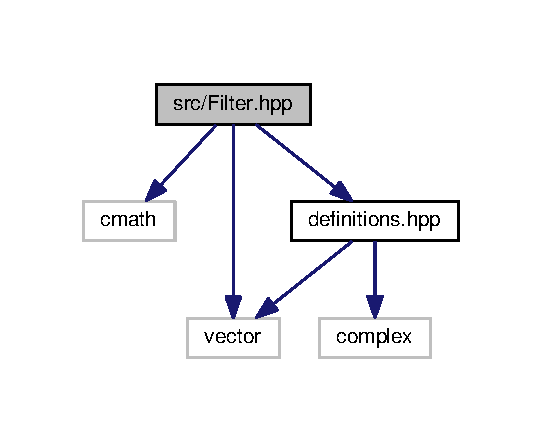
\includegraphics[width=260pt]{Filter_8hpp__incl}
\end{center}
\end{figure}
This graph shows which files directly or indirectly include this file\+:
\nopagebreak
\begin{figure}[H]
\begin{center}
\leavevmode
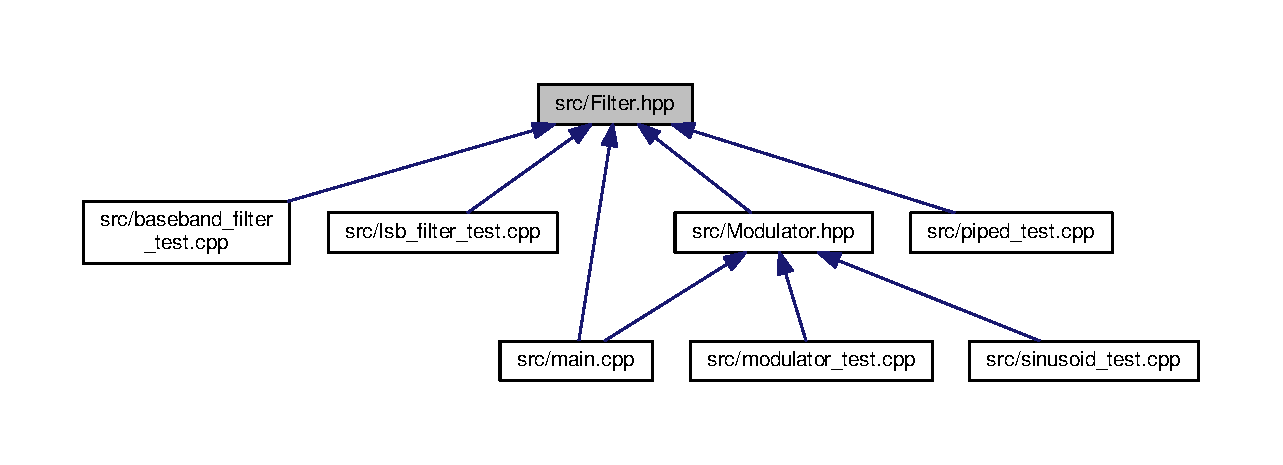
\includegraphics[width=350pt]{Filter_8hpp__dep__incl}
\end{center}
\end{figure}
\subsection*{Classes}
\begin{DoxyCompactItemize}
\item 
class \hyperlink{classradio_1_1Filter}{radio\+::\+Filter}
\end{DoxyCompactItemize}
\subsection*{Namespaces}
\begin{DoxyCompactItemize}
\item 
 \hyperlink{namespaceradio}{radio}
\begin{DoxyCompactList}\small\item\em contains helper-\/functions for \hyperlink{alsa__test_8cpp_ae66f6b31b5ad750f1fe042a706a4e3d4}{main()} \end{DoxyCompactList}\end{DoxyCompactItemize}


\subsection{Detailed Description}
Defines the Filter class. 

\begin{DoxyAuthor}{Author}
Samuel Andrew Wisner, \href{mailto:awisner94@gmail.com}{\tt awisner94@gmail.\+com} 
\end{DoxyAuthor}


Definition in file \hyperlink{Filter_8hpp_source}{Filter.\+hpp}.


\hypertarget{Filter_8hpp_source}{\section{Filter.\+hpp}
\label{Filter_8hpp_source}\index{src/\+Filter.\+hpp@{src/\+Filter.\+hpp}}
}

\begin{DoxyCode}
00001 
00008 \textcolor{preprocessor}{#ifndef Filter\_H}
00009 \textcolor{preprocessor}{#define Filter\_H}
00010 
00011 \textcolor{preprocessor}{#include <cmath>}
00012 \textcolor{preprocessor}{#include <vector>}
00013 
00014 \textcolor{preprocessor}{#include "\hyperlink{definitions_8hpp}{definitions.hpp}"}
00015 
00016 \textcolor{keyword}{namespace }\hyperlink{namespaceradio}{radio} \{
\hypertarget{Filter_8hpp_source_l00031}{}\hyperlink{classradio_1_1Filter}{00031}     \textcolor{keyword}{class }\hyperlink{classradio_1_1Filter}{Filter} \{
00032         \textcolor{keyword}{public}:
00047             \hyperlink{classradio_1_1Filter_a48ab268192e0135e5c9f74ad35a90fa1}{Filter}(\hyperlink{definitions_8hpp_aacdc525d6f7bddb3ae95d5c311bd06a1}{float32}* \hyperlink{classradio_1_1Filter_a25459a2b762120df0102f00553344be2}{data}, \hyperlink{definitions_8hpp_a1134b580f8da4de94ca6b1de4d37975e}{uint32} \hyperlink{classradio_1_1Filter_a7285b4c7263d8278e38abb14b5dca5d9}{size}, 
      \hyperlink{definitions_8hpp_a7615684c2af56be5f302c5b367d71f6b}{fparams}& \hyperlink{classradio_1_1Filter_abe705768a267844edfa2aaabfdac9f56}{diffEq});
00048 
00054             \textcolor{keywordtype}{void} \hyperlink{classradio_1_1Filter_ad2793821801780809af385463bf8f197}{Pass}();
00055 
00056         \textcolor{keyword}{protected}:
\hypertarget{Filter_8hpp_source_l00061}{}\hyperlink{classradio_1_1Filter_a26a32320c4dffa8925ab5f0f06689e8d}{00061}             \hyperlink{definitions_8hpp_adde6aaee8457bee49c2a92621fe22b79}{uint8} \hyperlink{classradio_1_1Filter_a26a32320c4dffa8925ab5f0f06689e8d}{eqLength};
00062 
\hypertarget{Filter_8hpp_source_l00066}{}\hyperlink{classradio_1_1Filter_a7285b4c7263d8278e38abb14b5dca5d9}{00066}             \hyperlink{definitions_8hpp_a1134b580f8da4de94ca6b1de4d37975e}{uint32} \hyperlink{classradio_1_1Filter_a7285b4c7263d8278e38abb14b5dca5d9}{size};
00067 
\hypertarget{Filter_8hpp_source_l00072}{}\hyperlink{classradio_1_1Filter_a25459a2b762120df0102f00553344be2}{00072}             \hyperlink{definitions_8hpp_aacdc525d6f7bddb3ae95d5c311bd06a1}{float32}* \hyperlink{classradio_1_1Filter_a25459a2b762120df0102f00553344be2}{data};
00073 
\hypertarget{Filter_8hpp_source_l00080}{}\hyperlink{classradio_1_1Filter_abe705768a267844edfa2aaabfdac9f56}{00080}             \hyperlink{definitions_8hpp_a7615684c2af56be5f302c5b367d71f6b}{fparams} \hyperlink{classradio_1_1Filter_abe705768a267844edfa2aaabfdac9f56}{diffEq};
00081     \};
00082 
\hypertarget{Filter_8hpp_source_l00083}{}\hyperlink{classradio_1_1Filter_a48ab268192e0135e5c9f74ad35a90fa1}{00083}     \hyperlink{classradio_1_1Filter_a48ab268192e0135e5c9f74ad35a90fa1}{Filter::Filter}(\hyperlink{definitions_8hpp_aacdc525d6f7bddb3ae95d5c311bd06a1}{float32}* data, \hyperlink{definitions_8hpp_a1134b580f8da4de94ca6b1de4d37975e}{uint32} size, 
      \hyperlink{definitions_8hpp_a7615684c2af56be5f302c5b367d71f6b}{fparams}& diffEq) \{
00084         this->data = \hyperlink{classradio_1_1Filter_a25459a2b762120df0102f00553344be2}{data};
00085         this->size = \hyperlink{classradio_1_1Filter_a7285b4c7263d8278e38abb14b5dca5d9}{size};
00086         this->diffEq = \hyperlink{classradio_1_1Filter_abe705768a267844edfa2aaabfdac9f56}{diffEq};
00087         \hyperlink{classradio_1_1Filter_a26a32320c4dffa8925ab5f0f06689e8d}{eqLength} = this->diffEq[\hyperlink{namespaceradio_aa2a4fb91116a2b9a094776a29cce0daca2fd2fe719e453d2bda50a402c0f49abe}{DEN}].size();
00088     \}
00089 
\hypertarget{Filter_8hpp_source_l00090}{}\hyperlink{classradio_1_1Filter_ad2793821801780809af385463bf8f197}{00090}     \textcolor{keywordtype}{void} \hyperlink{classradio_1_1Filter_ad2793821801780809af385463bf8f197}{Filter::Pass}() \{
00091         \hyperlink{definitions_8hpp_a232fad1b0d6dcc7c16aabde98b2e2a80}{float64} temp[\hyperlink{classradio_1_1Filter_a7285b4c7263d8278e38abb14b5dca5d9}{size}];
00092 
00093         \textcolor{comment}{// create first values in filtered data}
00094         \textcolor{keywordflow}{for}(\textcolor{keywordtype}{int} i = 0; i< \hyperlink{classradio_1_1Filter_a26a32320c4dffa8925ab5f0f06689e8d}{eqLength}; i++) \{
00095             temp[i] = 0;
00096 
00097             \textcolor{keywordflow}{for}(\textcolor{keywordtype}{int} j = 0; j < \hyperlink{classradio_1_1Filter_a26a32320c4dffa8925ab5f0f06689e8d}{eqLength}; j++) \{
00098                 temp[i] += \hyperlink{classradio_1_1Filter_abe705768a267844edfa2aaabfdac9f56}{diffEq}[\hyperlink{namespaceradio_aa2a4fb91116a2b9a094776a29cce0daca7436a425f0fd0f72aa39de328f2bdd48}{NUM}][j] * (j > i ? 0 : \hyperlink{classradio_1_1Filter_a25459a2b762120df0102f00553344be2}{data}[i - j]);
00099             \}
00100 
00101             \textcolor{keywordflow}{for}(\textcolor{keywordtype}{int} j = 1; j < \hyperlink{classradio_1_1Filter_a26a32320c4dffa8925ab5f0f06689e8d}{eqLength}; j++) \{
00102                 temp[i] -= \hyperlink{classradio_1_1Filter_abe705768a267844edfa2aaabfdac9f56}{diffEq}[\hyperlink{namespaceradio_aa2a4fb91116a2b9a094776a29cce0daca2fd2fe719e453d2bda50a402c0f49abe}{DEN}][j] * (j > i ? 0 : temp[i - j]);
00103             \}
00104         \}
00105 
00106         \textcolor{comment}{// create the REST of the values in filtered data}
00107         \textcolor{keywordflow}{for}(\textcolor{keywordtype}{int} i = eqLength; i < \hyperlink{classradio_1_1Filter_a7285b4c7263d8278e38abb14b5dca5d9}{size}; i++) \{
00108             temp[i] = 0;
00109 
00110             \textcolor{keywordflow}{for}(\textcolor{keywordtype}{int} j = 0; j < \hyperlink{classradio_1_1Filter_a26a32320c4dffa8925ab5f0f06689e8d}{eqLength}; j++) \{
00111                 temp[i] += \hyperlink{classradio_1_1Filter_abe705768a267844edfa2aaabfdac9f56}{diffEq}[\hyperlink{namespaceradio_aa2a4fb91116a2b9a094776a29cce0daca7436a425f0fd0f72aa39de328f2bdd48}{NUM}][j] * \hyperlink{classradio_1_1Filter_a25459a2b762120df0102f00553344be2}{data}[i - j];
00112             \}
00113 
00114             \textcolor{keywordflow}{for}(\textcolor{keywordtype}{int} j = 1; j < \hyperlink{classradio_1_1Filter_a26a32320c4dffa8925ab5f0f06689e8d}{eqLength}; j++) \{
00115                 temp[i] -= \hyperlink{classradio_1_1Filter_abe705768a267844edfa2aaabfdac9f56}{diffEq}[\hyperlink{namespaceradio_aa2a4fb91116a2b9a094776a29cce0daca2fd2fe719e453d2bda50a402c0f49abe}{DEN}][j] * temp[i - j];
00116             \}
00117         \}
00118 
00119         \textcolor{comment}{// save final values of data and filtered data}
00120     \textcolor{keywordflow}{for}(\textcolor{keywordtype}{int} i = 0; i < \hyperlink{classradio_1_1Filter_a7285b4c7263d8278e38abb14b5dca5d9}{size}; i++) \{
00121             \hyperlink{classradio_1_1Filter_a25459a2b762120df0102f00553344be2}{data}[i] = temp[i];
00122         \}
00123     \}
00124 \}
00125 
00126 \textcolor{preprocessor}{#endif}
\end{DoxyCode}

\hypertarget{fvectors_8hpp}{\section{src/fvectors.hpp File Reference}
\label{fvectors_8hpp}\index{src/fvectors.\+hpp@{src/fvectors.\+hpp}}
}


Defines the transfer function coefficients used in the instances of the Filter class in this program.  


{\ttfamily \#include $<$vector$>$}\\*
{\ttfamily \#include \char`\"{}definitions.\+hpp\char`\"{}}\\*
Include dependency graph for fvectors.\+hpp\+:
\nopagebreak
\begin{figure}[H]
\begin{center}
\leavevmode
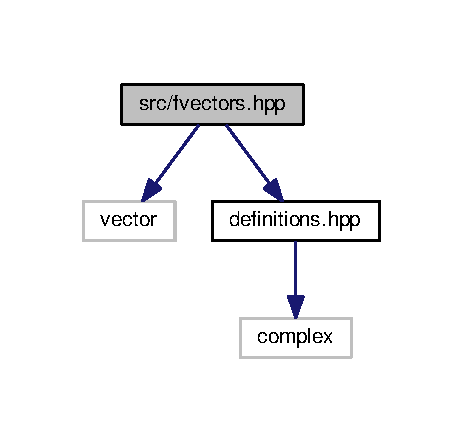
\includegraphics[width=222pt]{fvectors_8hpp__incl}
\end{center}
\end{figure}
This graph shows which files directly or indirectly include this file\+:
\nopagebreak
\begin{figure}[H]
\begin{center}
\leavevmode
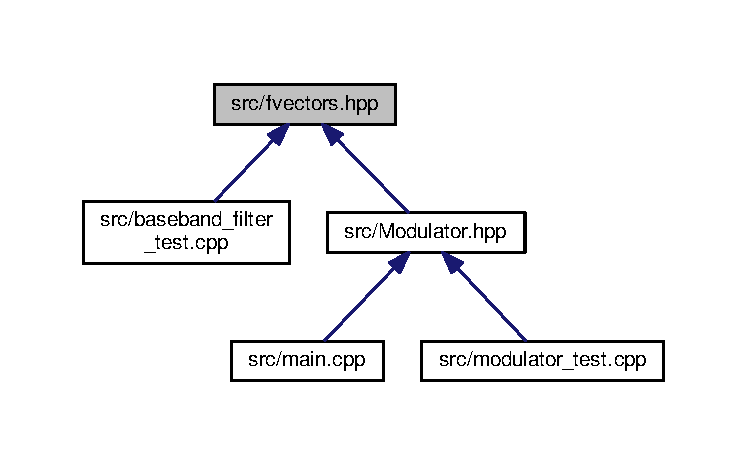
\includegraphics[width=296pt]{fvectors_8hpp__dep__incl}
\end{center}
\end{figure}
\subsection*{Namespaces}
\begin{DoxyCompactItemize}
\item 
 \hyperlink{namespaceradio}{radio}
\begin{DoxyCompactList}\small\item\em Contains the classes for the various types of modulation supported by the program. \end{DoxyCompactList}\end{DoxyCompactItemize}
\subsection*{Variables}
\begin{DoxyCompactItemize}
\item 
\hyperlink{definitions_8hpp_af19387f95516e2132a08cf60503f22a5}{fparams} \hyperlink{namespaceradio_a9bd902e9216499953a5906de73dc1796}{radio\+::\+F\+\_\+\+B\+A\+S\+E\+B\+A\+N\+D}
\item 
\hyperlink{definitions_8hpp_af19387f95516e2132a08cf60503f22a5}{fparams} \hyperlink{namespaceradio_a0ffd57d5a11ff70a1f55dbdc8ebe098d}{radio\+::\+F\+\_\+\+L\+O\+W\+E\+R\+S\+I\+D\+E\+B\+A\+N\+D}
\item 
\hyperlink{definitions_8hpp_af19387f95516e2132a08cf60503f22a5}{fparams} \hyperlink{namespaceradio_a0ec4548711b6d6ed6867c70b3fc2a413}{radio\+::\+F\+\_\+\+U\+P\+P\+E\+R\+S\+I\+D\+E\+B\+A\+N\+D}
\end{DoxyCompactItemize}


\subsection{Detailed Description}
Defines the transfer function coefficients used in the instances of the Filter class in this program. 

\begin{DoxyAuthor}{Author}
Samuel Andrew Wisner, \href{mailto:awisner94@gmail.com}{\tt awisner94@gmail.\+com} 
\end{DoxyAuthor}


Definition in file \hyperlink{fvectors_8hpp_source}{fvectors.\+hpp}.


\hypertarget{fvectors_8hpp_source}{\section{fvectors.\+hpp}
\label{fvectors_8hpp_source}\index{src/fvectors.\+hpp@{src/fvectors.\+hpp}}
}

\begin{DoxyCode}
00001 
00009 \textcolor{preprocessor}{#ifndef fvectors\_H}
00010 \textcolor{preprocessor}{#define fvectors\_H}
00011 
00012 \textcolor{preprocessor}{#include <vector>}
00013 
00014 \textcolor{preprocessor}{#include "\hyperlink{definitions_8hpp}{definitions.hpp}"}
00015 
00016 \textcolor{keyword}{namespace }\hyperlink{namespaceradio}{radio} \{
\hypertarget{fvectors_8hpp_source_l00020}{}\hyperlink{namespaceradio_a9bd902e9216499953a5906de73dc1796}{00020}     \hyperlink{definitions_8hpp_a7615684c2af56be5f302c5b367d71f6b}{fparams} \hyperlink{namespaceradio_a9bd902e9216499953a5906de73dc1796}{F\_BASEBAND} = \{ std::vector<float64> \{
00021         0.0008977019461,
00022             -0.002215694636,
00023             0.001372192986,
00024             0.001372192986,
00025             -0.002215694636,
00026             0.0008977019461 
00027     \}, std::vector<float64> \{
00028         1,
00029             -4.678616047,
00030             8.822912216,
00031             -8.379911423,
00032             4.007629871,
00033             -0.7719064355
00034     \} \};
00035 
\hypertarget{fvectors_8hpp_source_l00039}{}\hyperlink{namespaceradio_a0ffd57d5a11ff70a1f55dbdc8ebe098d}{00039}     \hyperlink{definitions_8hpp_a7615684c2af56be5f302c5b367d71f6b}{fparams} \hyperlink{namespaceradio_a0ffd57d5a11ff70a1f55dbdc8ebe098d}{F\_LOWERSIDEBAND} = \{ std::vector<float64> \{
00040         0.2758039069174,   
00041             2.763578787693,   
00042             12.83915022756,   
00043             36.47584850651,
00044             70.37084637368,   
00045             96.76893503179,   
00046             96.76893503179,   
00047             70.37084637368,
00048             36.47584850651,   
00049             12.83915022756,   
00050             2.763578787693,  
00051             0.2758039069174   
00052     \}, std::vector<float64> \{
00053         1,
00054             7.605497780083,   
00055             27.34180552438,   
00056             60.83375457605,
00057             92.60908886875,       
00058             100.8363857,    
00059             79.74796574736,     
00060             45.4982252145,
00061             18.13566776308,    
00062             4.690036472717,   
00063             0.6617552879305,   
00064             0.0281427334611
00065     \} \};
00066 
\hypertarget{fvectors_8hpp_source_l00070}{}\hyperlink{namespaceradio_a0ec4548711b6d6ed6867c70b3fc2a413}{00070}     \hyperlink{definitions_8hpp_a7615684c2af56be5f302c5b367d71f6b}{fparams} \hyperlink{namespaceradio_a0ec4548711b6d6ed6867c70b3fc2a413}{F\_UPPERSIDEBAND} = \{ std::vector<float64> \{
00071         0.001690387681463, 
00072             0.01145271586989, 
00073             0.03591799189724, 
00074             0.06576926098562,
00075             0.07119343282702,
00076             0.03156377419766,
00077             -0.03156377419766,
00078             -0.07119343282702,
00079             -0.06576926098562,
00080             -0.03591799189724,
00081             -0.01145271586989,
00082             -0.001690387681463
00083     \}, std::vector<float64> \{
00084         1,  
00085             9.465175013624,
00086             41.62402815905,
00087             112.0971027069,
00088             205.2097686473,    
00089             267.9378582311,     
00090             254.486805213,
00091             175.7772755115,
00092             86.51619894548,   
00093             28.89988093561,     
00094             5.89781461091,
00095             0.5572910543053   
00096     \} \};
00097 
00098 
00099 \}
00100 
00101 \textcolor{preprocessor}{#endif}
\end{DoxyCode}

\hypertarget{Gain_8hpp}{\section{src/\+Gain.hpp File Reference}
\label{Gain_8hpp}\index{src/\+Gain.\+hpp@{src/\+Gain.\+hpp}}
}


Contains the Gain class.  


{\ttfamily \#include $<$cmath$>$}\\*
{\ttfamily \#include \char`\"{}definitions.\+hpp\char`\"{}}\\*
Include dependency graph for Gain.\+hpp\+:
\nopagebreak
\begin{figure}[H]
\begin{center}
\leavevmode
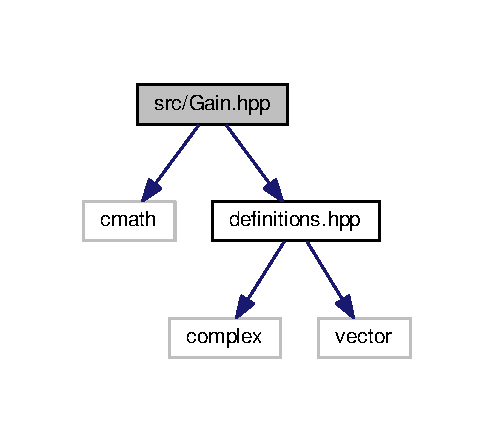
\includegraphics[width=237pt]{Gain_8hpp__incl}
\end{center}
\end{figure}
This graph shows which files directly or indirectly include this file\+:
\nopagebreak
\begin{figure}[H]
\begin{center}
\leavevmode
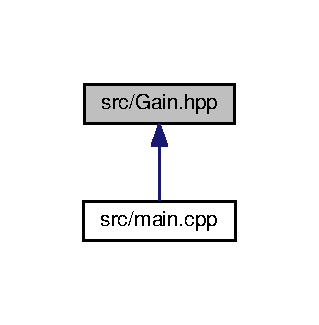
\includegraphics[width=153pt]{Gain_8hpp__dep__incl}
\end{center}
\end{figure}
\subsection*{Classes}
\begin{DoxyCompactItemize}
\item 
class \hyperlink{classradio_1_1Gain}{radio\+::\+Gain}
\end{DoxyCompactItemize}
\subsection*{Namespaces}
\begin{DoxyCompactItemize}
\item 
 \hyperlink{namespaceradio}{radio}
\end{DoxyCompactItemize}


\subsection{Detailed Description}
Contains the Gain class. 

\begin{DoxyAuthor}{Author}
Samuel Andrew Wisner, \href{mailto:awisner94@gmail.com}{\tt awisner94@gmail.\+com} 
\end{DoxyAuthor}


Definition in file \hyperlink{Gain_8hpp_source}{Gain.\+hpp}.


\hypertarget{Gain_8hpp_source}{\section{Gain.\+hpp}
\label{Gain_8hpp_source}\index{src/\+Gain.\+hpp@{src/\+Gain.\+hpp}}
}

\begin{DoxyCode}
00001 
00007 \textcolor{preprocessor}{#ifndef Gain\_H}
00008 \textcolor{preprocessor}{#define Gain\_H}
00009 
00010 \textcolor{preprocessor}{#include <cmath>}
00011 
00012 \textcolor{preprocessor}{#include "\hyperlink{definitions_8hpp}{definitions.hpp}"}
00013 
00014 \textcolor{keyword}{namespace }\hyperlink{namespaceradio}{radio} \{
\hypertarget{Gain_8hpp_source_l00018}{}\hyperlink{classradio_1_1Gain}{00018}     \textcolor{keyword}{class }\hyperlink{classradio_1_1Gain}{Gain} \{
00019         \textcolor{keyword}{public}:
00030             \hyperlink{classradio_1_1Gain_a11f137515c0ecc04333c7d92eea2cf79}{Gain}(\hyperlink{definitions_8hpp_aacdc525d6f7bddb3ae95d5c311bd06a1}{float32}* data, \hyperlink{definitions_8hpp_a1134b580f8da4de94ca6b1de4d37975e}{uint32} size, \hyperlink{definitions_8hpp_aacdc525d6f7bddb3ae95d5c311bd06a1}{float32} gaindB);
00031 
00035             \textcolor{keywordtype}{void} \hyperlink{classradio_1_1Gain_a8c6df2c5989da0e560c8f276e6138a2d}{Apply}();
00036 
00037         \textcolor{keyword}{private}:
00041             \hyperlink{definitions_8hpp_aacdc525d6f7bddb3ae95d5c311bd06a1}{float32}* data;
00042 
00046             \hyperlink{definitions_8hpp_aacdc525d6f7bddb3ae95d5c311bd06a1}{float32} gainCoeff;
00047 
00052             \textcolor{keywordtype}{bool} hasClipped = \textcolor{keyword}{false};
00053 
00057             \hyperlink{definitions_8hpp_a1134b580f8da4de94ca6b1de4d37975e}{uint32} size;
00058 
00059     \};
00060 
\hypertarget{Gain_8hpp_source_l00061}{}\hyperlink{classradio_1_1Gain_a11f137515c0ecc04333c7d92eea2cf79}{00061}     \hyperlink{classradio_1_1Gain_a11f137515c0ecc04333c7d92eea2cf79}{Gain::Gain}(\hyperlink{definitions_8hpp_aacdc525d6f7bddb3ae95d5c311bd06a1}{float32}* data, \hyperlink{definitions_8hpp_a1134b580f8da4de94ca6b1de4d37975e}{uint32} size, \hyperlink{definitions_8hpp_aacdc525d6f7bddb3ae95d5c311bd06a1}{float32} gaindB) \{
00062         this->data = data;
00063         this->size = size;
00064         gainCoeff = pow(10, gaindB / 20);
00065     \}
00066 
\hypertarget{Gain_8hpp_source_l00067}{}\hyperlink{classradio_1_1Gain_a8c6df2c5989da0e560c8f276e6138a2d}{00067}     \textcolor{keywordtype}{void} \hyperlink{classradio_1_1Gain_a8c6df2c5989da0e560c8f276e6138a2d}{Gain::Apply}() \{
00068         \textcolor{keywordflow}{for}(\hyperlink{definitions_8hpp_a1134b580f8da4de94ca6b1de4d37975e}{uint32} i = 0; i < size; i++) \{
00069             data[i] *= gainCoeff;
00070 
00071             \textcolor{keywordflow}{if}((data[i] > 1 || data[i] < -1) && !hasClipped) \{
00072                 hasClipped = \textcolor{keyword}{true};
00073                 std::cerr << \textcolor{stringliteral}{"Baseband clipping has occurred!"}
00074                     << std::endl;
00075             \}
00076         \}
00077     \}
00078 \}
00079 
00080 \textcolor{preprocessor}{#endif}
\end{DoxyCode}

\hypertarget{iq__test_8cpp}{\section{src/iq\+\_\+test.cpp File Reference}
\label{iq__test_8cpp}\index{src/iq\+\_\+test.\+cpp@{src/iq\+\_\+test.\+cpp}}
}


Generates test I\+Q signal.  


{\ttfamily \#include $<$iostream$>$}\\*
{\ttfamily \#include $<$cstdio$>$}\\*
{\ttfamily \#include $<$unistd.\+h$>$}\\*
{\ttfamily \#include \char`\"{}zdomain.\+hpp\char`\"{}}\\*
Include dependency graph for iq\+\_\+test.\+cpp\+:
\nopagebreak
\begin{figure}[H]
\begin{center}
\leavevmode
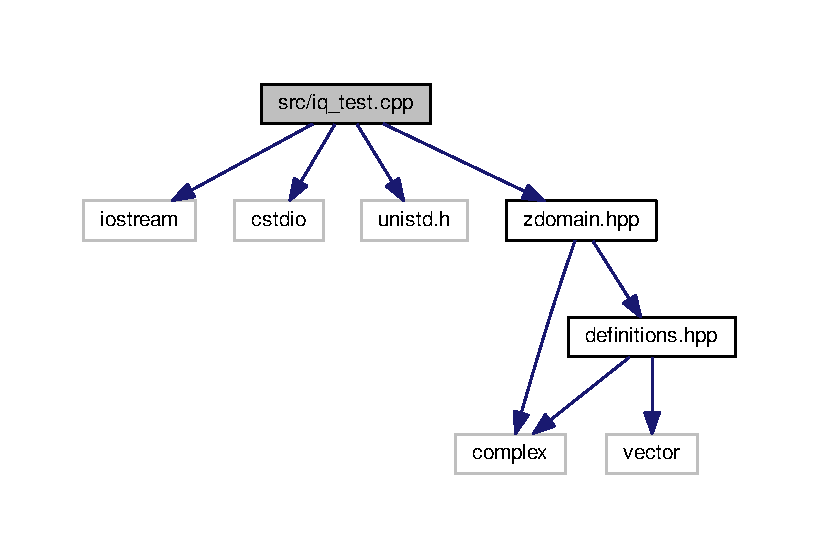
\includegraphics[width=350pt]{iq__test_8cpp__incl}
\end{center}
\end{figure}
\subsection*{Functions}
\begin{DoxyCompactItemize}
\item 
int \hyperlink{iq__test_8cpp_ae66f6b31b5ad750f1fe042a706a4e3d4}{main} ()
\end{DoxyCompactItemize}


\subsection{Detailed Description}
Generates test I\+Q signal. 

\begin{DoxyAuthor}{Author}
Samuel Andrew Wisner, \href{mailto:awisner94@gmail.com}{\tt awisner94@gmail.\+com} 
\end{DoxyAuthor}


Definition in file \hyperlink{iq__test_8cpp_source}{iq\+\_\+test.\+cpp}.



\subsection{Function Documentation}
\hypertarget{iq__test_8cpp_ae66f6b31b5ad750f1fe042a706a4e3d4}{\index{iq\+\_\+test.\+cpp@{iq\+\_\+test.\+cpp}!main@{main}}
\index{main@{main}!iq\+\_\+test.\+cpp@{iq\+\_\+test.\+cpp}}
\subsubsection[{main}]{\setlength{\rightskip}{0pt plus 5cm}int main (
\begin{DoxyParamCaption}
{}
\end{DoxyParamCaption}
)}}\label{iq__test_8cpp_ae66f6b31b5ad750f1fe042a706a4e3d4}
This small program demonstrates the I\+Q generation abilities of the \hyperlink{namespaceradio_a7166522e76ff88e8d482491b1b6e2275}{make\+I\+Q()} function. 

Definition at line 20 of file iq\+\_\+test.\+cpp.



Here is the call graph for this function\+:
\nopagebreak
\begin{figure}[H]
\begin{center}
\leavevmode
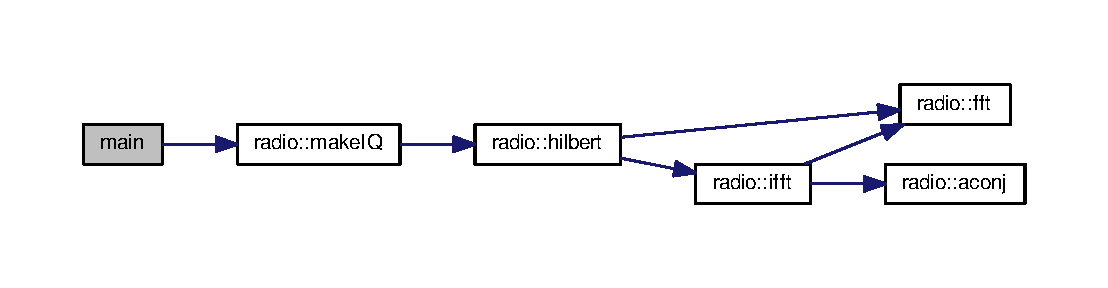
\includegraphics[width=350pt]{iq__test_8cpp_ae66f6b31b5ad750f1fe042a706a4e3d4_cgraph}
\end{center}
\end{figure}



\hypertarget{iq__test_8cpp_source}{\section{iq\+\_\+test.\+cpp}
\label{iq__test_8cpp_source}\index{src/iq\+\_\+test.\+cpp@{src/iq\+\_\+test.\+cpp}}
}

\begin{DoxyCode}
00001 
00007 \textcolor{preprocessor}{#include <iostream>}
00008 \textcolor{preprocessor}{#include <cstdio>}
00009 \textcolor{preprocessor}{#include <unistd.h>}
00010 
00011 \textcolor{preprocessor}{#include "\hyperlink{zdomain_8hpp}{zdomain.hpp}"}
00012 
00013 \textcolor{keyword}{using namespace }\hyperlink{namespacestd}{std};
00014 \textcolor{keyword}{using namespace }\hyperlink{namespaceradio}{radio};
00015 
\hypertarget{iq__test_8cpp_source_l00020}{}\hyperlink{iq__test_8cpp_ae66f6b31b5ad750f1fe042a706a4e3d4}{00020} \textcolor{keywordtype}{int} \hyperlink{iq__test_8cpp_ae66f6b31b5ad750f1fe042a706a4e3d4}{main}() \{
00021     \textcolor{keyword}{const} \hyperlink{definitions_8hpp_a05f6b0ae8f6a6e135b0e290c25fe0e4e}{uint16} len = 16384;
00022     \hyperlink{definitions_8hpp_aacdc525d6f7bddb3ae95d5c311bd06a1}{float32} data[len];
00023     \hyperlink{definitions_8hpp_aacdc525d6f7bddb3ae95d5c311bd06a1}{float32} iqData[2*len];
00024 
00025     \textcolor{keywordflow}{for}(\textcolor{keywordtype}{int} i = 0; i < len; i++) \{
00026         data[i] = sin(2*3.141592*170*i/len);
00027     \}
00028 
00029     \textcolor{keywordflow}{while}(\textcolor{keyword}{true}) \{
00030         read(STDIN\_FILENO, &data, len * \textcolor{keyword}{sizeof}(\hyperlink{definitions_8hpp_aacdc525d6f7bddb3ae95d5c311bd06a1}{float32}));
00031         \hyperlink{namespaceradio_a7166522e76ff88e8d482491b1b6e2275}{makeIQ}(data, iqData, len);
00032         write(STDOUT\_FILENO, &iqData,  2 * len * \textcolor{keyword}{sizeof}(\hyperlink{definitions_8hpp_aacdc525d6f7bddb3ae95d5c311bd06a1}{float32}));
00033     \}
00034 \}
\end{DoxyCode}

\hypertarget{lsb__filter__test_8cpp}{\section{src/lsb\+\_\+filter\+\_\+test.cpp File Reference}
\label{lsb__filter__test_8cpp}\index{src/lsb\+\_\+filter\+\_\+test.\+cpp@{src/lsb\+\_\+filter\+\_\+test.\+cpp}}
}


contains a program to test the L\+S\+B-\/via-\/filter implementation  


{\ttfamily \#include $<$iostream$>$}\\*
{\ttfamily \#include $<$cmath$>$}\\*
{\ttfamily \#include $<$cstdio$>$}\\*
{\ttfamily \#include $<$unistd.\+h$>$}\\*
{\ttfamily \#include \char`\"{}definitions.\+hpp\char`\"{}}\\*
{\ttfamily \#include \char`\"{}Filter.\+hpp\char`\"{}}\\*
{\ttfamily \#include \char`\"{}fvectors.\+hpp\char`\"{}}\\*
{\ttfamily \#include \char`\"{}zdomain.\+hpp\char`\"{}}\\*
Include dependency graph for lsb\+\_\+filter\+\_\+test.\+cpp\+:
\nopagebreak
\begin{figure}[H]
\begin{center}
\leavevmode
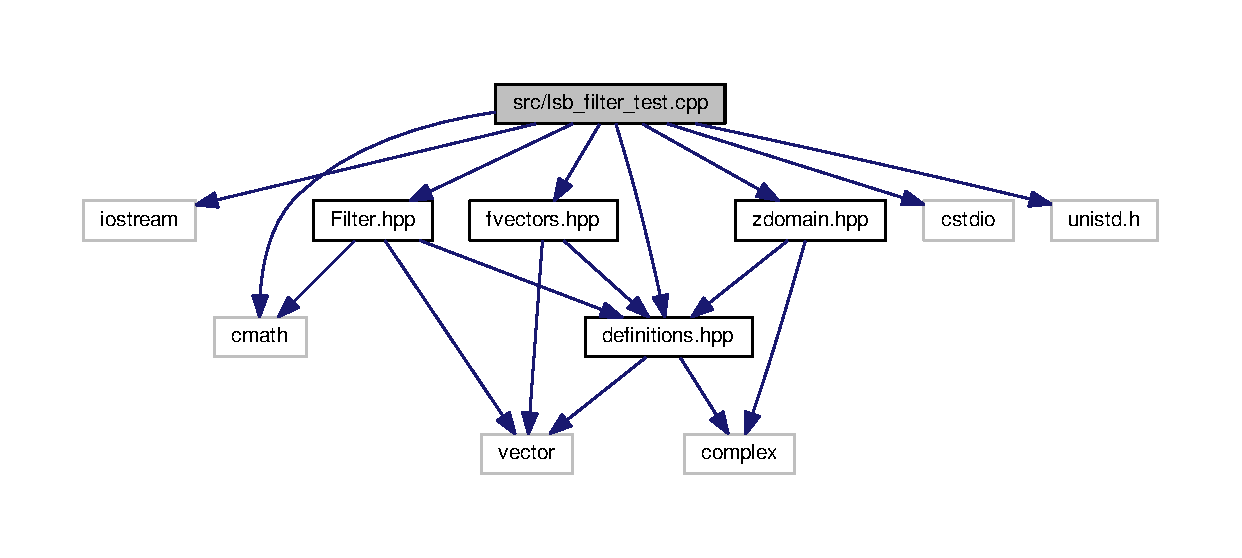
\includegraphics[width=350pt]{lsb__filter__test_8cpp__incl}
\end{center}
\end{figure}
\subsection*{Functions}
\begin{DoxyCompactItemize}
\item 
int \hyperlink{lsb__filter__test_8cpp_ae66f6b31b5ad750f1fe042a706a4e3d4}{main} ()
\end{DoxyCompactItemize}


\subsection{Detailed Description}
contains a program to test the L\+S\+B-\/via-\/filter implementation 

\begin{DoxyAuthor}{Author}
Samuel Andrew Wisner, \href{mailto:awisner94@gmail.com}{\tt awisner94@gmail.\+com} 
\end{DoxyAuthor}


Definition in file \hyperlink{lsb__filter__test_8cpp_source}{lsb\+\_\+filter\+\_\+test.\+cpp}.



\subsection{Function Documentation}
\hypertarget{lsb__filter__test_8cpp_ae66f6b31b5ad750f1fe042a706a4e3d4}{\index{lsb\+\_\+filter\+\_\+test.\+cpp@{lsb\+\_\+filter\+\_\+test.\+cpp}!main@{main}}
\index{main@{main}!lsb\+\_\+filter\+\_\+test.\+cpp@{lsb\+\_\+filter\+\_\+test.\+cpp}}
\subsubsection[{main}]{\setlength{\rightskip}{0pt plus 5cm}int main (
\begin{DoxyParamCaption}
{}
\end{DoxyParamCaption}
)}}\label{lsb__filter__test_8cpp_ae66f6b31b5ad750f1fe042a706a4e3d4}
Tests an implementation of L\+S\+B modulation through a filter. 

Definition at line 23 of file lsb\+\_\+filter\+\_\+test.\+cpp.



Here is the call graph for this function\+:
\nopagebreak
\begin{figure}[H]
\begin{center}
\leavevmode
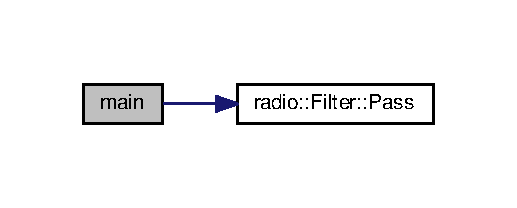
\includegraphics[width=248pt]{lsb__filter__test_8cpp_ae66f6b31b5ad750f1fe042a706a4e3d4_cgraph}
\end{center}
\end{figure}



\hypertarget{lsb__filter__test_8cpp_source}{\section{lsb\+\_\+filter\+\_\+test.\+cpp}
\label{lsb__filter__test_8cpp_source}\index{src/lsb\+\_\+filter\+\_\+test.\+cpp@{src/lsb\+\_\+filter\+\_\+test.\+cpp}}
}

\begin{DoxyCode}
00001 
00007 \textcolor{preprocessor}{#include <cstdio>}
00008 \textcolor{preprocessor}{#include <cstdlib>}
00009 \textcolor{preprocessor}{#include <iostream>}
00010 \textcolor{preprocessor}{#include <unistd.h>}
00011 
00012 \textcolor{preprocessor}{#include "\hyperlink{auxiliary_8hpp}{auxiliary.hpp}"}
00013 \textcolor{preprocessor}{#include "\hyperlink{definitions_8hpp}{definitions.hpp}"}
00014 \textcolor{preprocessor}{#include "\hyperlink{Filter_8hpp}{Filter.hpp}"}
00015 \textcolor{preprocessor}{#include "\hyperlink{fvectors_8hpp}{fvectors.hpp}"}
00016 \textcolor{preprocessor}{#include "\hyperlink{Sinusoid_8hpp}{Sinusoid.hpp}"}
00017 \textcolor{preprocessor}{#include "\hyperlink{zdomain_8hpp}{zdomain.hpp}"}
00018 
00019 \textcolor{keyword}{using namespace }\hyperlink{namespacestd}{std};
00020 \textcolor{keyword}{using namespace }\hyperlink{namespaceradio}{radio};
00021 
\hypertarget{lsb__filter__test_8cpp_source_l00025}{}\hyperlink{lsb__filter__test_8cpp_a0ddf1224851353fc92bfbff6f499fa97}{00025} \textcolor{keywordtype}{int} \hyperlink{lsb__filter__test_8cpp_a0ddf1224851353fc92bfbff6f499fa97}{main}(\textcolor{keywordtype}{int} argc, \textcolor{keywordtype}{char}* argv[]) \{
00026 
00027     \textcolor{comment}{// Constants}
00028     \textcolor{keyword}{const} \hyperlink{definitions_8hpp_a05f6b0ae8f6a6e135b0e290c25fe0e4e}{uint16} BUFFER\_SIZE = 48000;
00029 
00030     \textcolor{comment}{// Declare primative Variables}
00031     \hyperlink{definitions_8hpp_adde6aaee8457bee49c2a92621fe22b79}{uint8} i = 0;
00032     \hyperlink{definitions_8hpp_adde6aaee8457bee49c2a92621fe22b79}{uint8} size = 0;
00033     \hyperlink{definitions_8hpp_a05f6b0ae8f6a6e135b0e290c25fe0e4e}{uint16} delta = 250;
00034     \hyperlink{definitions_8hpp_aacdc525d6f7bddb3ae95d5c311bd06a1}{float32} dataBuffer[BUFFER\_SIZE];
00035     \hyperlink{definitions_8hpp_aacdc525d6f7bddb3ae95d5c311bd06a1}{float32} iqBuffer[2 * BUFFER\_SIZE];
00036 
00037     \textcolor{comment}{// create 1 sec of audio}
00038     \textcolor{keywordflow}{for}(\hyperlink{definitions_8hpp_a05f6b0ae8f6a6e135b0e290c25fe0e4e}{uint16} f = 17000; f <= 23000; f += delta, i++) \{
00039         \hyperlink{classradio_1_1Sinusoid}{Sinusoid} sinusoid(f);
00040 
00041         \textcolor{keywordflow}{for}(\hyperlink{definitions_8hpp_a05f6b0ae8f6a6e135b0e290c25fe0e4e}{uint16} i = 0; i < BUFFER\_SIZE; i++) \{
00042             dataBuffer[i] += sinusoid.\hyperlink{classradio_1_1Sinusoid_aab44298ea1bd5cb175d5826243cf56f2}{next}();
00043         \}
00044     \}
00045 
00046     size = i;
00047     
00048     \textcolor{comment}{// adjust dataBuffer so values are between -1 and 1}
00049     \textcolor{keywordflow}{for}(\hyperlink{definitions_8hpp_a05f6b0ae8f6a6e135b0e290c25fe0e4e}{uint16} i = 0; i < BUFFER\_SIZE; i++) \{
00050         dataBuffer[i] /= size;
00051     \}
00052     
00053     \hyperlink{classradio_1_1Filter}{Filter} filter(dataBuffer, BUFFER\_SIZE, \hyperlink{namespaceradio_a0ffd57d5a11ff70a1f55dbdc8ebe098d}{F\_LOWERSIDEBAND});
00054     filter.\hyperlink{classradio_1_1Filter_ad2793821801780809af385463bf8f197}{Pass}();
00055     \hyperlink{namespaceradio_a7166522e76ff88e8d482491b1b6e2275}{makeIQ}(dataBuffer, iqBuffer, BUFFER\_SIZE);
00056     \hyperlink{namespaceradio_ae4b2334c4366dcdf0311ad79d2067945}{to\_sint32}(iqBuffer, 2 * BUFFER\_SIZE);
00057 
00058     \textcolor{keywordflow}{while}(\textcolor{keyword}{true}) \{
00059         write(STDOUT\_FILENO, &iqBuffer, 2 * BUFFER\_SIZE * \textcolor{keyword}{sizeof}(\hyperlink{definitions_8hpp_a0573de65958b4fda3a0460ed417dafb8}{sint32}));
00060     \}
00061 \}
\end{DoxyCode}

\hypertarget{main_8cpp}{\section{src/main.cpp File Reference}
\label{main_8cpp}\index{src/main.\+cpp@{src/main.\+cpp}}
}


contains the \char`\"{}brains\char`\"{} of the entire project  


{\ttfamily \#include $<$cstdio$>$}\\*
{\ttfamily \#include $<$iostream$>$}\\*
{\ttfamily \#include $<$stdexcept$>$}\\*
{\ttfamily \#include $<$string$>$}\\*
{\ttfamily \#include $<$unistd.\+h$>$}\\*
{\ttfamily \#include \char`\"{}auxiliary.\+hpp\char`\"{}}\\*
{\ttfamily \#include \char`\"{}Filter.\+hpp\char`\"{}}\\*
{\ttfamily \#include \char`\"{}Gain.\+hpp\char`\"{}}\\*
{\ttfamily \#include \char`\"{}Modulator.\+hpp\char`\"{}}\\*
{\ttfamily \#include \char`\"{}Pl\+Tone.\+hpp\char`\"{}}\\*
{\ttfamily \#include \char`\"{}zdomain.\+hpp\char`\"{}}\\*
Include dependency graph for main.\+cpp\+:
\nopagebreak
\begin{figure}[H]
\begin{center}
\leavevmode
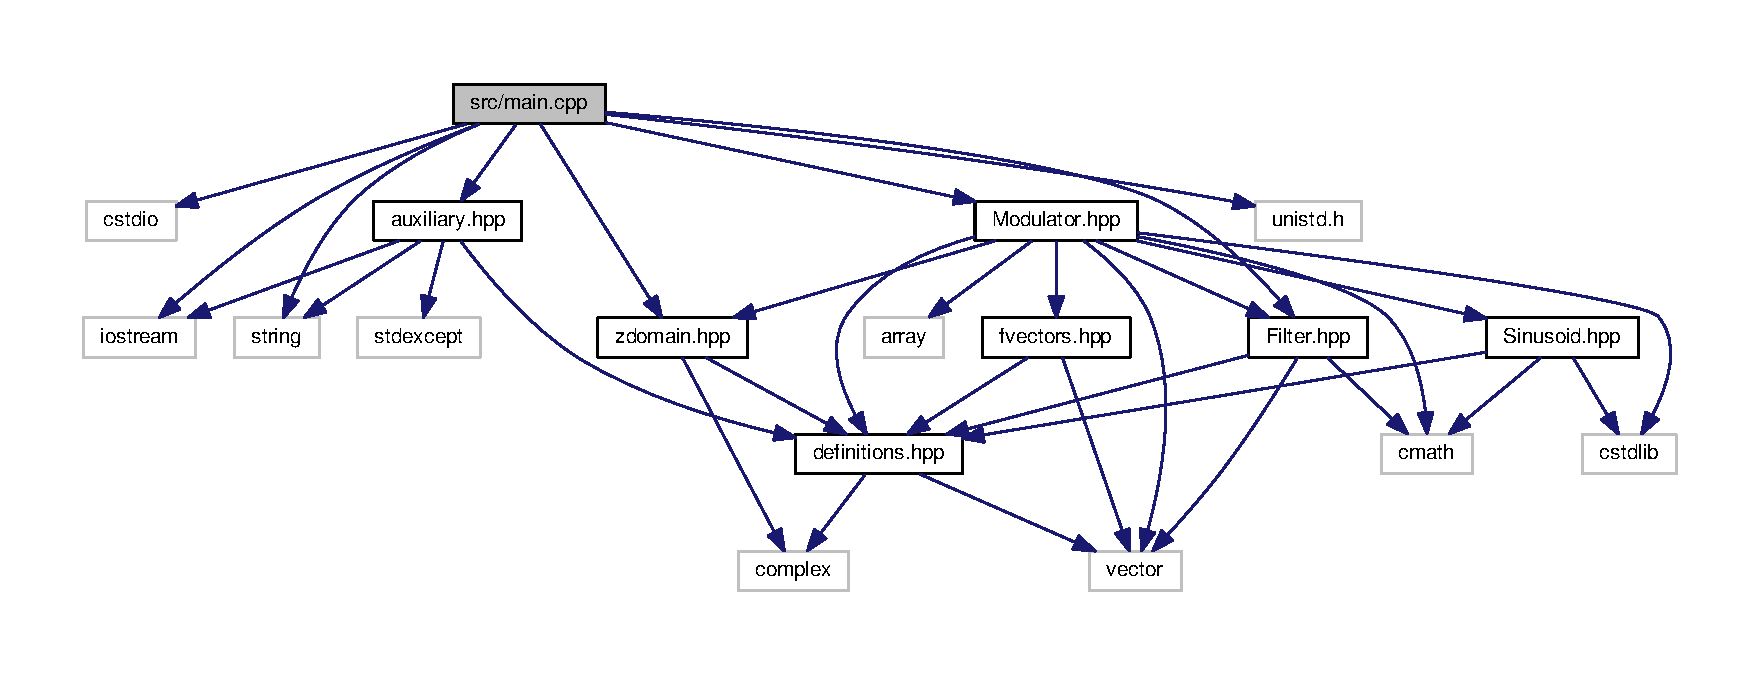
\includegraphics[width=350pt]{main_8cpp__incl}
\end{center}
\end{figure}
\subsection*{Functions}
\begin{DoxyCompactItemize}
\item 
int \hyperlink{main_8cpp_a0ddf1224851353fc92bfbff6f499fa97}{main} (int argc, char $\ast$argv\mbox{[}$\,$\mbox{]})
\end{DoxyCompactItemize}


\subsection{Detailed Description}
contains the \char`\"{}brains\char`\"{} of the entire project 

\begin{DoxyAuthor}{Author}
Samuel Andrew Wisner, \href{mailto:awisner94@gmail.com}{\tt awisner94@gmail.\+com} 
\end{DoxyAuthor}


Definition in file \hyperlink{main_8cpp_source}{main.\+cpp}.



\subsection{Function Documentation}
\hypertarget{main_8cpp_a0ddf1224851353fc92bfbff6f499fa97}{\index{main.\+cpp@{main.\+cpp}!main@{main}}
\index{main@{main}!main.\+cpp@{main.\+cpp}}
\subsubsection[{main}]{\setlength{\rightskip}{0pt plus 5cm}int main (
\begin{DoxyParamCaption}
\item[{int}]{argc, }
\item[{char $\ast$}]{argv\mbox{[}$\,$\mbox{]}}
\end{DoxyParamCaption}
)}}\label{main_8cpp_a0ddf1224851353fc92bfbff6f499fa97}
Final result of the entire project. Completes all goals and more! 

Definition at line 26 of file main.\+cpp.



Here is the call graph for this function\+:
\nopagebreak
\begin{figure}[H]
\begin{center}
\leavevmode
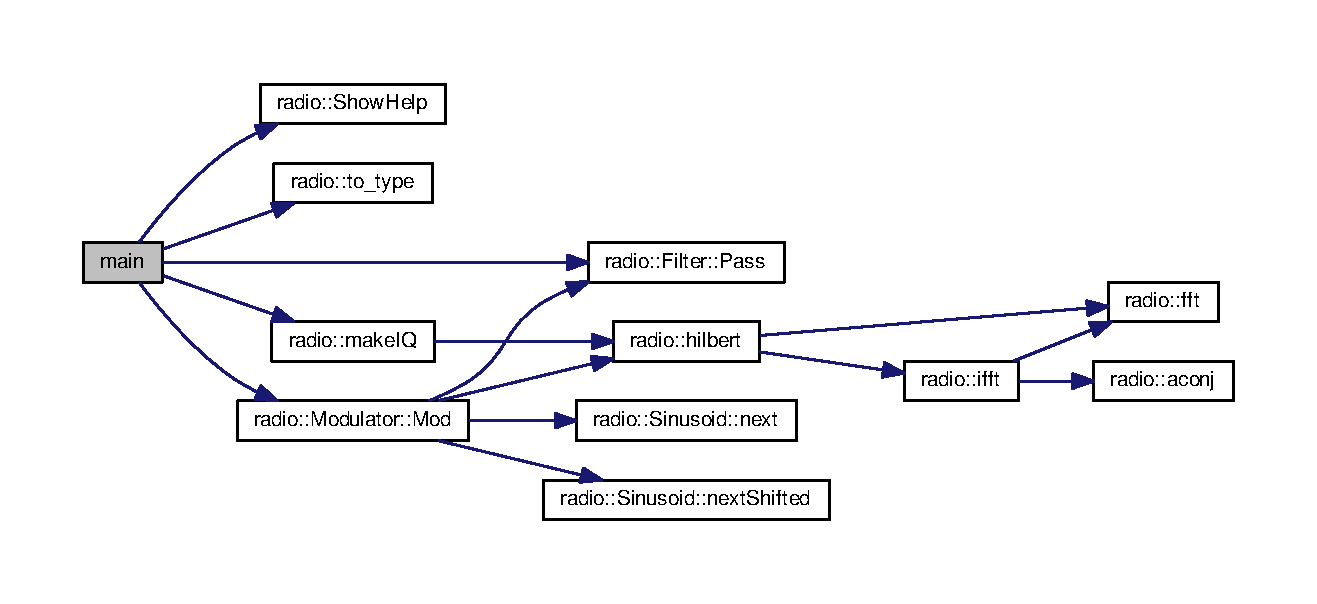
\includegraphics[width=350pt]{main_8cpp_a0ddf1224851353fc92bfbff6f499fa97_cgraph}
\end{center}
\end{figure}



\hypertarget{main_8cpp_source}{\section{main.\+cpp}
\label{main_8cpp_source}\index{src/main.\+cpp@{src/main.\+cpp}}
}

\begin{DoxyCode}
00001 
00007 \textcolor{preprocessor}{#include <cstdio>}
00008 \textcolor{preprocessor}{#include <iostream>}
00009 \textcolor{preprocessor}{#include <stdexcept>}
00010 \textcolor{preprocessor}{#include <string>}
00011 \textcolor{preprocessor}{#include <unistd.h>}
00012 
00013 \textcolor{preprocessor}{#include "\hyperlink{auxiliary_8hpp}{auxiliary.hpp}"}
00014 \textcolor{preprocessor}{#include "\hyperlink{Filter_8hpp}{Filter.hpp}"}
00015 \textcolor{preprocessor}{#include "\hyperlink{Gain_8hpp}{Gain.hpp}"}
00016 \textcolor{preprocessor}{#include "\hyperlink{Modulator_8hpp}{Modulator.hpp}"}
00017 \textcolor{preprocessor}{#include "\hyperlink{PlTone_8hpp}{PlTone.hpp}"}
00018 \textcolor{preprocessor}{#include "\hyperlink{zdomain_8hpp}{zdomain.hpp}"}
00019 
00020 \textcolor{keyword}{using namespace }\hyperlink{namespacestd}{std};
00021 \textcolor{keyword}{using namespace }\hyperlink{namespaceradio}{radio};
00022 
\hypertarget{main_8cpp_source_l00026}{}\hyperlink{main_8cpp_a0ddf1224851353fc92bfbff6f499fa97}{00026} \textcolor{keywordtype}{int} \hyperlink{main_8cpp_a0ddf1224851353fc92bfbff6f499fa97}{main}(\textcolor{keywordtype}{int} argc, \textcolor{keywordtype}{char}* argv[]) \{
00027 
00028     \textcolor{comment}{// Constants}
00029     \textcolor{keyword}{const} \hyperlink{definitions_8hpp_adde6aaee8457bee49c2a92621fe22b79}{uint8} NUM\_TYPES = 8;
00030     \textcolor{keyword}{const} \hyperlink{definitions_8hpp_a05f6b0ae8f6a6e135b0e290c25fe0e4e}{uint16} BUFFER\_SIZE = 16384;
00031     \textcolor{keyword}{const} \hyperlink{definitions_8hpp_a1134b580f8da4de94ca6b1de4d37975e}{uint32} BUFFER\_BYTE\_COUNT = BUFFER\_SIZE * \textcolor{keyword}{sizeof}(\hyperlink{definitions_8hpp_a0573de65958b4fda3a0460ed417dafb8}{sint32});
00032     \textcolor{keyword}{const} \hyperlink{definitions_8hpp_a1134b580f8da4de94ca6b1de4d37975e}{uint32} IQ\_BUFFER\_SIZE = 2 * BUFFER\_SIZE;
00033     \textcolor{keyword}{const} \hyperlink{definitions_8hpp_a1134b580f8da4de94ca6b1de4d37975e}{uint32} IQ\_BUFFER\_BYTE\_COUNT = BUFFER\_BYTE\_COUNT * 2;
00034     \textcolor{keyword}{const} \hyperlink{definitions_8hpp_a1134b580f8da4de94ca6b1de4d37975e}{uint32} \hyperlink{namespaceradio_a284213fea4beed2f74bb936927cbe654}{SAMPLING\_RATE} = 48000;
00035 
00036     \textcolor{comment}{// Ensure 1 or 2 arguments given}
00037     \textcolor{keywordflow}{if}(argc > 4) \{
00038         std::cerr << \textcolor{stringliteral}{"Error: too many arguments!"} << std::endl;
00039         \hyperlink{namespaceradio_a6db7c682d0f9aeac8cb5042717b8ae7f}{ShowHelp}();
00040         \textcolor{keywordflow}{return} \hyperlink{definitions_8hpp_a8fe83ac76edc595f6b98cd4a4127aed5}{ERROR};
00041     \} \textcolor{keywordflow}{else} \textcolor{keywordflow}{if}(argc < 2) \{
00042         std::cerr << \textcolor{stringliteral}{"Error: too few arguments!"} << std::endl;
00043         \hyperlink{namespaceradio_a6db7c682d0f9aeac8cb5042717b8ae7f}{ShowHelp}();
00044         \textcolor{keywordflow}{return} \hyperlink{definitions_8hpp_a8fe83ac76edc595f6b98cd4a4127aed5}{ERROR};
00045     \}
00046 
00047     \textcolor{comment}{// Declare primative Variables}
00048     \hyperlink{definitions_8hpp_aacdc525d6f7bddb3ae95d5c311bd06a1}{float32} micGain = 0;
00049     \hyperlink{definitions_8hpp_aacdc525d6f7bddb3ae95d5c311bd06a1}{float32} toneFreq = 0;
00050     \hyperlink{definitions_8hpp_aacdc525d6f7bddb3ae95d5c311bd06a1}{float32} dataBuffer[BUFFER\_SIZE];
00051     \hyperlink{definitions_8hpp_aacdc525d6f7bddb3ae95d5c311bd06a1}{float32} iqBuffer[IQ\_BUFFER\_SIZE];
00052     \hyperlink{namespaceradio_a46fb7299001138f28b7f69975c58399e}{ModulationType} type;
00053 
00054     \textcolor{comment}{// validate modulation type}
00055     \textcolor{keywordflow}{try}\{
00056         type = \hyperlink{namespaceradio_a402fe28e2e2bb2be7a0d2d9f74cc640d}{to\_type}(\textcolor{keywordtype}{string}(argv[1]));
00057     \} \textcolor{keywordflow}{catch}(std::exception ex) \{
00058         std::cerr << \textcolor{stringliteral}{"The given modulation type is invalid!"} << std::endl;
00059         \hyperlink{namespaceradio_a6db7c682d0f9aeac8cb5042717b8ae7f}{ShowHelp}();
00060     \}
00061 
00062     \textcolor{comment}{// process mic gain}
00063     \textcolor{keywordflow}{if}(argc >= 3) \{
00064         \textcolor{keywordflow}{try} \{
00065             micGain = std::stof(argv[2]);
00066         \} \textcolor{keywordflow}{catch}(std::invalid\_argument ex) \{
00067             std::cerr << \textcolor{stringliteral}{"The specified microphone gain is not a number."}
00068                 << std::endl;
00069             \hyperlink{namespaceradio_a6db7c682d0f9aeac8cb5042717b8ae7f}{ShowHelp}();
00070         \}
00071     \}
00072 
00073     \textcolor{comment}{// validate CTCSS tone}
00074     \textcolor{keywordflow}{if}(argc == 4) \{
00075         \textcolor{keywordflow}{try} \{
00076             toneFreq = std::stof(argv[3]);
00077 
00078             \textcolor{keywordflow}{if}(toneFreq < 60 || toneFreq > 260) \{
00079                 \textcolor{keywordflow}{throw} std::out\_of\_range(\textcolor{stringliteral}{""});
00080             \}
00081         \} \textcolor{keywordflow}{catch}(std::out\_of\_range ex) \{
00082             std::cerr << \textcolor{stringliteral}{"The specified CTCSS frequency is outside of the "}
00083                 \textcolor{stringliteral}{"standard PL tone range."} << std::endl;
00084             \hyperlink{namespaceradio_a6db7c682d0f9aeac8cb5042717b8ae7f}{ShowHelp}();
00085         \} \textcolor{keywordflow}{catch}(std::invalid\_argument ex) \{
00086             std::cerr << \textcolor{stringliteral}{"The specified CTCSS frequency is not a number."}
00087                 << std::endl;
00088             \hyperlink{namespaceradio_a6db7c682d0f9aeac8cb5042717b8ae7f}{ShowHelp}();
00089         \}
00090     \}
00091 
00092     \textcolor{comment}{// Declare objects}
00093     \hyperlink{classradio_1_1Filter}{Filter} baseFilter(dataBuffer, BUFFER\_SIZE, \hyperlink{namespaceradio_a9bd902e9216499953a5906de73dc1796}{F\_BASEBAND});
00094     \hyperlink{classradio_1_1Gain}{Gain} gain(dataBuffer, BUFFER\_SIZE, micGain);
00095     \hyperlink{classradio_1_1PlTone}{PlTone} pltone(0.15, dataBuffer, BUFFER\_SIZE, toneFreq, SAMPLING\_RATE);
00096     \hyperlink{classradio_1_1Modulator}{Modulator} modulator(dataBuffer, BUFFER\_SIZE, type, 20000);
00097 
00098     \textcolor{comment}{// SDR guts of the program}
00099     \textcolor{keywordflow}{while}(\textcolor{keyword}{true}) \{
00100         \textcolor{comment}{// get next samples}
00101         read(STDIN\_FILENO, &dataBuffer, BUFFER\_BYTE\_COUNT);
00102         
00103         \textcolor{comment}{// process/modulate samples}
00104         baseFilter.\hyperlink{classradio_1_1Filter_ad2793821801780809af385463bf8f197}{Pass}();
00105 \textcolor{comment}{//      pltone.Add();}
00106         gain.\hyperlink{classradio_1_1Gain_a8c6df2c5989da0e560c8f276e6138a2d}{Apply}();
00107         modulator.\hyperlink{classradio_1_1Modulator_ab5eac6e4900579486b5871b48e64cdab}{Mod}();
00108         \hyperlink{namespaceradio_a7166522e76ff88e8d482491b1b6e2275}{makeIQ}(dataBuffer, iqBuffer, BUFFER\_SIZE);
00109         \hyperlink{namespaceradio_ae4b2334c4366dcdf0311ad79d2067945}{to\_sint32}(iqBuffer, IQ\_BUFFER\_SIZE);
00110         
00111         \textcolor{comment}{// write samples}
00112         write(STDOUT\_FILENO, &iqBuffer, IQ\_BUFFER\_BYTE\_COUNT);
00113     \}
00114 \}
\end{DoxyCode}

\hypertarget{mic__test_8cpp}{\section{src/mic\+\_\+test.cpp File Reference}
\label{mic__test_8cpp}\index{src/mic\+\_\+test.\+cpp@{src/mic\+\_\+test.\+cpp}}
}


Tests getting mic input via A\+L\+S\+A  May not even compile at the moment.  


{\ttfamily \#include $<$cmath$>$}\\*
{\ttfamily \#include $<$climits$>$}\\*
{\ttfamily \#include $<$iostream$>$}\\*
{\ttfamily \#include $<$alsa/asoundlib.\+h$>$}\\*
{\ttfamily \#include \char`\"{}definitions.\+hpp\char`\"{}}\\*
Include dependency graph for mic\+\_\+test.\+cpp\+:
\nopagebreak
\begin{figure}[H]
\begin{center}
\leavevmode
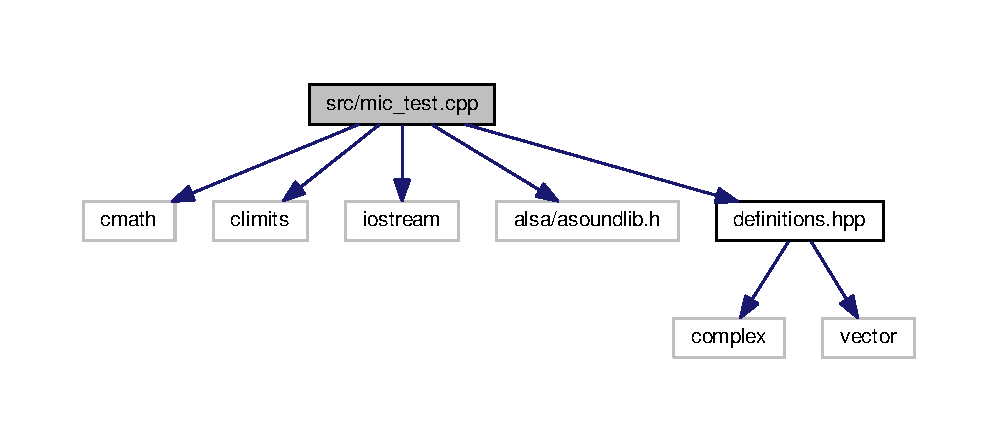
\includegraphics[width=350pt]{mic__test_8cpp__incl}
\end{center}
\end{figure}
\subsection*{Functions}
\begin{DoxyCompactItemize}
\item 
int \hyperlink{mic__test_8cpp_ae66f6b31b5ad750f1fe042a706a4e3d4}{main} ()
\end{DoxyCompactItemize}


\subsection{Detailed Description}
Tests getting mic input via A\+L\+S\+A  May not even compile at the moment. 

\begin{DoxyAuthor}{Author}
Samuel Andrew Wisner, \href{mailto:awisner94@gmail.com}{\tt awisner94@gmail.\+com} 
\end{DoxyAuthor}


Definition in file \hyperlink{mic__test_8cpp_source}{mic\+\_\+test.\+cpp}.



\subsection{Function Documentation}
\hypertarget{mic__test_8cpp_ae66f6b31b5ad750f1fe042a706a4e3d4}{\index{mic\+\_\+test.\+cpp@{mic\+\_\+test.\+cpp}!main@{main}}
\index{main@{main}!mic\+\_\+test.\+cpp@{mic\+\_\+test.\+cpp}}
\subsubsection[{main}]{\setlength{\rightskip}{0pt plus 5cm}int main (
\begin{DoxyParamCaption}
{}
\end{DoxyParamCaption}
)}}\label{mic__test_8cpp_ae66f6b31b5ad750f1fe042a706a4e3d4}
This program tests taking information from the microphone via the A\+L\+S\+A A\+P\+I. Not sure if it works. 

Definition at line \hyperlink{mic__test_8cpp_source_l00021}{21} of file \hyperlink{mic__test_8cpp_source}{mic\+\_\+test.\+cpp}.


\hypertarget{mic__test_8cpp_source}{\section{mic\+\_\+test.\+cpp}
\label{mic__test_8cpp_source}\index{src/mic\+\_\+test.\+cpp@{src/mic\+\_\+test.\+cpp}}
}

\begin{DoxyCode}
00001 
00008 \textcolor{preprocessor}{#include <cmath>}
00009 \textcolor{preprocessor}{#include <climits>}
00010 \textcolor{preprocessor}{#include <iostream>}
00011 \textcolor{preprocessor}{#include <alsa/asoundlib.h>}
00012 
00013 \textcolor{preprocessor}{#include "\hyperlink{definitions_8hpp}{definitions.hpp}"}
00014 
00015 \textcolor{keyword}{using namespace }\hyperlink{namespacestd}{std};
00016 
\hypertarget{mic__test_8cpp_source_l00021}{}\hyperlink{mic__test_8cpp_ae66f6b31b5ad750f1fe042a706a4e3d4}{00021} \textcolor{keywordtype}{int} \hyperlink{mic__test_8cpp_ae66f6b31b5ad750f1fe042a706a4e3d4}{main}() \{
00022     \textcolor{keywordtype}{int} ret;
00023 
00024     snd\_pcm\_t* pcm\_handle;  \textcolor{comment}{// device handle}
00025 \textcolor{comment}{//  snd\_pcm\_stream\_t stream = SND\_PCM\_STREAM\_PLAYBACK;}
00026     snd\_pcm\_stream\_t stream = SND\_PCM\_STREAM\_CAPTURE;
00027     snd\_pcm\_hw\_params\_t* hwparams;  \textcolor{comment}{// hardware information}
00028     \textcolor{keywordtype}{char}* pcm\_name = strdup(\textcolor{stringliteral}{"plughw:1,0"});  \textcolor{comment}{// on-board audio jack}
00029     \textcolor{comment}{//char* pcm\_name = strdup("plughw:0,0");  // on-board audio jack}
00030     \textcolor{keywordtype}{int} rate = 48000;
00031 
00032     \textcolor{keyword}{const} \hyperlink{definitions_8hpp_a05f6b0ae8f6a6e135b0e290c25fe0e4e}{uint16} freq = 440;
00033     \textcolor{keywordtype}{long} \textcolor{keywordtype}{unsigned} \textcolor{keywordtype}{int} bufferSize = 8192*4;
00034     \textcolor{keyword}{const} \hyperlink{definitions_8hpp_a1134b580f8da4de94ca6b1de4d37975e}{uint32} len = bufferSize*100;
00035     \textcolor{keyword}{const} \hyperlink{definitions_8hpp_aacdc525d6f7bddb3ae95d5c311bd06a1}{float32} arg = 2 * 3.141592 * freq / rate;
00036     \hyperlink{definitions_8hpp_a74df79fde3c518e55b29ce6360a9c76e}{sint16} vals[len];
00037 
00038     \textcolor{keywordtype}{float} test;
00039     \textcolor{keywordtype}{float} last = 0;
00040     \textcolor{keywordtype}{long} \textcolor{keywordtype}{unsigned} \textcolor{keywordtype}{int} count = 0;
00041     \textcolor{keywordtype}{int} count2 = 0;
00042 
00043     \textcolor{keywordflow}{for}(\textcolor{keywordtype}{int} i = 0; i < len; i = i + 2) \{
00044         \textcolor{keywordtype}{bool} lastWas = abs(sin(last)) < 0.01;
00045 
00046         last += arg;
00047         \textcolor{keywordflow}{if}(last > 2 * M\_PI) last -= 2 * M\_PI;
00048 
00049         test = 32000 * sin(last);
00050 
00051         \textcolor{keywordflow}{if}(abs(sin(last)) < 0.01 && lastWas) count++;
00052 
00053         vals[i] = (\hyperlink{definitions_8hpp_a74df79fde3c518e55b29ce6360a9c76e}{sint16})(test + 0.5);
00054         vals[i+1] = vals[i];
00055     \}
00056 
00057     cout << \textcolor{stringliteral}{"COUNT: "} << count << endl;
00058     snd\_pcm\_hw\_params\_alloca(&hwparams);
00059 
00060     ret = snd\_pcm\_open(&pcm\_handle, pcm\_name, stream, 0);
00061     cout << \textcolor{stringliteral}{"Opening: "} << snd\_strerror(ret) << endl;
00062 
00063     ret = snd\_pcm\_hw\_params\_any(pcm\_handle, hwparams);
00064     cout << \textcolor{stringliteral}{"Initializing hwparams structure: "} << snd\_strerror(ret) << endl;   
00065 
00066     ret = snd\_pcm\_hw\_params\_set\_access(pcm\_handle, hwparams,
00067             SND\_PCM\_ACCESS\_RW\_INTERLEAVED);
00068     cout << \textcolor{stringliteral}{"Setting access: "} << snd\_strerror(ret) << endl;
00069 
00070     ret = snd\_pcm\_hw\_params\_set\_format(pcm\_handle, hwparams,
00071             SND\_PCM\_FORMAT\_S16\_LE);
00072     cout << \textcolor{stringliteral}{"Setting format: "} << snd\_strerror(ret) << endl;
00073 
00074     ret = snd\_pcm\_hw\_params\_set\_rate(pcm\_handle, hwparams,
00075             rate, (\textcolor{keywordtype}{int})0);
00076     cout << \textcolor{stringliteral}{"Setting rate: "} << snd\_strerror(ret) << endl;
00077 
00078     ret = snd\_pcm\_hw\_params\_set\_channels(pcm\_handle, hwparams, 2); 
00079     cout << \textcolor{stringliteral}{"Setting channels: "} << snd\_strerror(ret) << endl;
00080 
00081     ret = snd\_pcm\_hw\_params\_set\_periods(pcm\_handle, hwparams, 2, 0);
00082     cout << \textcolor{stringliteral}{"Setting periods: "} << snd\_strerror(ret) << endl;
00083 
00084     ret = snd\_pcm\_hw\_params\_set\_buffer\_size\_near(pcm\_handle, hwparams,
00085             &bufferSize);
00086     cout << \textcolor{stringliteral}{"Setting buffer size: "} << snd\_strerror(ret) << endl;
00087 
00088     ret = snd\_pcm\_hw\_params(pcm\_handle, hwparams);
00089     cout << \textcolor{stringliteral}{"Applying parameters: "} << snd\_strerror(ret) << endl;
00090 
00091 \textcolor{comment}{/*  ret = snd\_pcm\_hw\_params\_get\_period\_size(hwparams, &count, &count2);}
00092 \textcolor{comment}{    cout << "Actual period size: " << count << endl;}
00093 \textcolor{comment}{    cout << "Returned: " << snd\_strerror(ret) << endl;*/}
00094 
00095     
00096 
00097     cout << endl << endl;
00098 
00099 
00100     \textcolor{comment}{//const void* ptr = (const void*)&vals;}
00101     \textcolor{keywordtype}{void}* ptr = (\textcolor{keywordtype}{void}*)&vals;
00102     \textcolor{keywordtype}{int} err;
00103 
00104     \textcolor{keywordflow}{for}(\textcolor{keywordtype}{int} i = 0; i < 100; i++) \{
00105         \textcolor{keywordflow}{do} \{
00106             ret = snd\_pcm\_readi(pcm\_handle,
00107                     ptr, bufferSize);
00108 
00109             \textcolor{keywordflow}{if}(ret < 0) \{
00110                 err = snd\_pcm\_prepare(pcm\_handle);
00111                 cout << \textcolor{stringliteral}{"Preparing: "} << snd\_strerror(err)
00112                     << endl;
00113             \}
00114         \} \textcolor{keywordflow}{while}(ret < 0);
00115 
00116         cout << \textcolor{stringliteral}{"Writing data: "} << ret << endl;
00117     \}
00118 \}
\end{DoxyCode}

\hypertarget{Modulator_8hpp}{\section{src/\+Modulator.hpp File Reference}
\label{Modulator_8hpp}\index{src/\+Modulator.\+hpp@{src/\+Modulator.\+hpp}}
}
{\ttfamily \#include $<$array$>$}\\*
{\ttfamily \#include $<$cmath$>$}\\*
{\ttfamily \#include $<$cstdlib$>$}\\*
{\ttfamily \#include $<$vector$>$}\\*
{\ttfamily \#include \char`\"{}definitions.\+hpp\char`\"{}}\\*
{\ttfamily \#include \char`\"{}Filter.\+hpp\char`\"{}}\\*
{\ttfamily \#include \char`\"{}fvectors.\+hpp\char`\"{}}\\*
{\ttfamily \#include \char`\"{}Sinusoid.\+hpp\char`\"{}}\\*
{\ttfamily \#include \char`\"{}zdomain.\+hpp\char`\"{}}\\*
Include dependency graph for Modulator.\+hpp\+:
\nopagebreak
\begin{figure}[H]
\begin{center}
\leavevmode
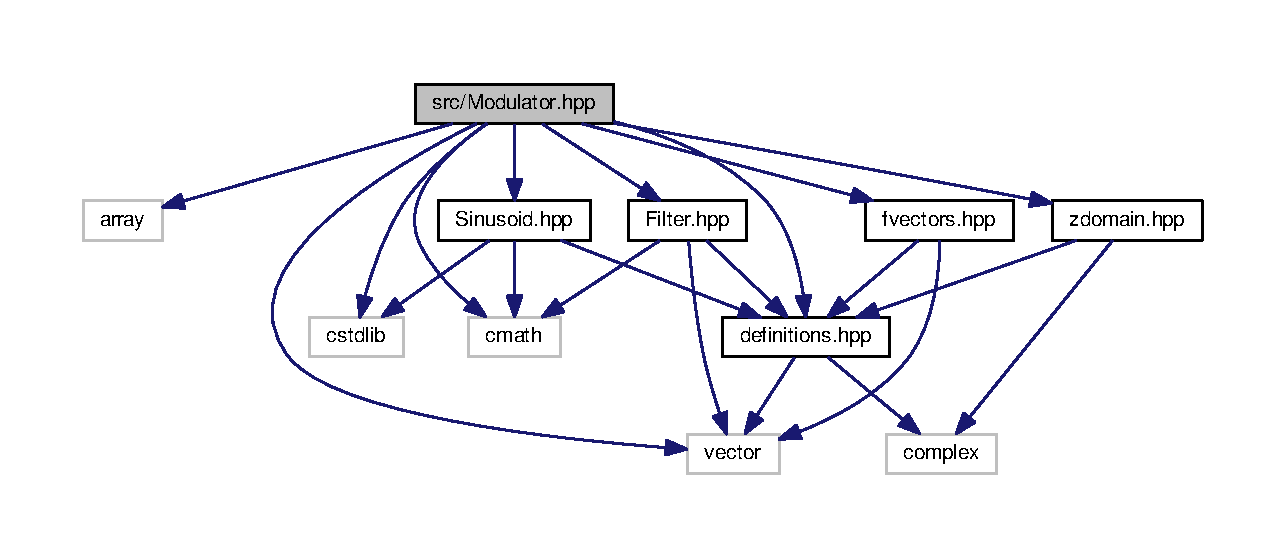
\includegraphics[width=350pt]{Modulator_8hpp__incl}
\end{center}
\end{figure}
This graph shows which files directly or indirectly include this file\+:
\nopagebreak
\begin{figure}[H]
\begin{center}
\leavevmode
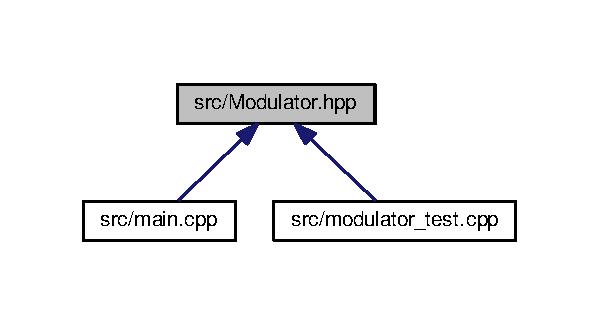
\includegraphics[width=288pt]{Modulator_8hpp__dep__incl}
\end{center}
\end{figure}
\subsection*{Classes}
\begin{DoxyCompactItemize}
\item 
class \hyperlink{classradio_1_1Modulator}{radio\+::\+Modulator}
\end{DoxyCompactItemize}
\subsection*{Namespaces}
\begin{DoxyCompactItemize}
\item 
 \hyperlink{namespaceradio}{radio}
\begin{DoxyCompactList}\small\item\em contains helper-\/functions for \hyperlink{alsa__test_8cpp_ae66f6b31b5ad750f1fe042a706a4e3d4}{main()} \end{DoxyCompactList}\end{DoxyCompactItemize}
\subsection*{Variables}
\begin{DoxyCompactItemize}
\item 
const \hyperlink{definitions_8hpp_a1134b580f8da4de94ca6b1de4d37975e}{uint32} \hyperlink{namespaceradio_aa82ddc6ba206798fd70ffc25665b3cb6}{radio\+::\+F\+R\+E\+Q\+\_\+\+I\+N\+T\+E\+R\+M\+E\+D\+I\+A\+T\+E} = 20000
\item 
const \hyperlink{definitions_8hpp_a1134b580f8da4de94ca6b1de4d37975e}{uint32} \hyperlink{namespaceradio_a284213fea4beed2f74bb936927cbe654}{radio\+::\+S\+A\+M\+P\+L\+I\+N\+G\+\_\+\+R\+A\+T\+E} = 48000
\end{DoxyCompactItemize}

\hypertarget{Modulator_8hpp_source}{\section{Modulator.\+hpp}
\label{Modulator_8hpp_source}\index{src/\+Modulator.\+hpp@{src/\+Modulator.\+hpp}}
}

\begin{DoxyCode}
00001 
00009 \textcolor{preprocessor}{#ifndef modulation\_H}
00010 \textcolor{preprocessor}{#define modulation\_H}
00011 
00012 \textcolor{preprocessor}{#include <array>}
00013 \textcolor{preprocessor}{#include <cmath>}
00014 \textcolor{preprocessor}{#include <cstdlib>}
00015 \textcolor{preprocessor}{#include <vector>}
00016 
00017 \textcolor{preprocessor}{#include "\hyperlink{definitions_8hpp}{definitions.hpp}"}
00018 \textcolor{preprocessor}{#include "\hyperlink{Filter_8hpp}{Filter.hpp}"}
00019 \textcolor{preprocessor}{#include "\hyperlink{fvectors_8hpp}{fvectors.hpp}"}
00020 \textcolor{preprocessor}{#include "\hyperlink{Sinusoid_8hpp}{Sinusoid.hpp}"}
00021 \textcolor{preprocessor}{#include "\hyperlink{zdomain_8hpp}{zdomain.hpp}"}
00022 
00023 \textcolor{keyword}{namespace }\hyperlink{namespaceradio}{radio} \{
00024 
\hypertarget{Modulator_8hpp_source_l00028}{}\hyperlink{namespaceradio_aa82ddc6ba206798fd70ffc25665b3cb6}{00028}     \textcolor{keyword}{const} \hyperlink{definitions_8hpp_a1134b580f8da4de94ca6b1de4d37975e}{uint32} \hyperlink{namespaceradio_aa82ddc6ba206798fd70ffc25665b3cb6}{FREQ\_INTERMEDIATE} = 20000;
00029 
\hypertarget{Modulator_8hpp_source_l00033}{}\hyperlink{namespaceradio_a284213fea4beed2f74bb936927cbe654}{00033}     \textcolor{keyword}{const} \hyperlink{definitions_8hpp_a1134b580f8da4de94ca6b1de4d37975e}{uint32} \hyperlink{namespaceradio_a284213fea4beed2f74bb936927cbe654}{SAMPLING\_RATE} = 48000;
00034 
\hypertarget{Modulator_8hpp_source_l00039}{}\hyperlink{classradio_1_1Modulator}{00039}     \textcolor{keyword}{class }\hyperlink{classradio_1_1Modulator}{Modulator} \{
00040         \textcolor{keyword}{public}:
00055             \hyperlink{classradio_1_1Modulator_ab202651b368986cc76673b6e997550b8}{Modulator}(\hyperlink{definitions_8hpp_aacdc525d6f7bddb3ae95d5c311bd06a1}{float32} data[], \hyperlink{definitions_8hpp_a1134b580f8da4de94ca6b1de4d37975e}{uint32} size, 
      \hyperlink{namespaceradio_a46fb7299001138f28b7f69975c58399e}{ModulationType} type,
00056                     \hyperlink{definitions_8hpp_aacdc525d6f7bddb3ae95d5c311bd06a1}{float32} freqInter = FREQ\_INTERMEDIATE,
00057                     \hyperlink{definitions_8hpp_a1134b580f8da4de94ca6b1de4d37975e}{uint32} rate = SAMPLING\_RATE);
00058 
00062             \hyperlink{classradio_1_1Modulator_a712e6e110c57b29ebdd754bd34bf269b}{~Modulator}();
00063 
00067             \textcolor{keywordtype}{void} \hyperlink{classradio_1_1Modulator_ab5eac6e4900579486b5871b48e64cdab}{Mod}();
00068 
00069         \textcolor{keyword}{private}:
00074             \hyperlink{definitions_8hpp_aacdc525d6f7bddb3ae95d5c311bd06a1}{float32}* data;
00075 
00079             \hyperlink{definitions_8hpp_aacdc525d6f7bddb3ae95d5c311bd06a1}{float32} freqCarrier;
00080 
00081 
00085             \hyperlink{definitions_8hpp_aacdc525d6f7bddb3ae95d5c311bd06a1}{float32}* hilData = \textcolor{keyword}{nullptr};
00086 
00090             \hyperlink{definitions_8hpp_aacdc525d6f7bddb3ae95d5c311bd06a1}{float32} rate;
00091 
00095             \hyperlink{definitions_8hpp_a1134b580f8da4de94ca6b1de4d37975e}{uint32} size;
00096 
00100             \hyperlink{namespaceradio_a46fb7299001138f28b7f69975c58399e}{ModulationType} type;
00101     \};
00102 
\hypertarget{Modulator_8hpp_source_l00103}{}\hyperlink{classradio_1_1Modulator_ab202651b368986cc76673b6e997550b8}{00103}     \hyperlink{classradio_1_1Modulator_ab202651b368986cc76673b6e997550b8}{Modulator::Modulator}(\hyperlink{definitions_8hpp_aacdc525d6f7bddb3ae95d5c311bd06a1}{float32} data[], \hyperlink{definitions_8hpp_a1134b580f8da4de94ca6b1de4d37975e}{uint32} size, 
      \hyperlink{namespaceradio_a46fb7299001138f28b7f69975c58399e}{ModulationType} type,
00104             \hyperlink{definitions_8hpp_aacdc525d6f7bddb3ae95d5c311bd06a1}{float32} freqInter, \hyperlink{definitions_8hpp_a1134b580f8da4de94ca6b1de4d37975e}{uint32} rate) \{
00105         freqCarrier = freqInter;
00106         this->rate = rate;
00107         this->data = data;
00108         this->size = size;
00109         this->type = type;
00110 
00111         \textcolor{keywordflow}{if}(type == \hyperlink{namespaceradio_a46fb7299001138f28b7f69975c58399ea1b14284e455bf5c311de662665312d13}{ModulationType::USB\_HILBERT}
00112                 || type == \hyperlink{namespaceradio_a46fb7299001138f28b7f69975c58399ea18f970daa5b5a8f72cbd45f7b49a6b6a}{ModulationType::LSB\_HILBERT}) \{
00113             hilData = (\hyperlink{definitions_8hpp_aacdc525d6f7bddb3ae95d5c311bd06a1}{float32}*)malloc(size*\textcolor{keyword}{sizeof}(\hyperlink{definitions_8hpp_aacdc525d6f7bddb3ae95d5c311bd06a1}{float32}));
00114         \}
00115     \}
00116 
\hypertarget{Modulator_8hpp_source_l00117}{}\hyperlink{classradio_1_1Modulator_a712e6e110c57b29ebdd754bd34bf269b}{00117}     \hyperlink{classradio_1_1Modulator_a712e6e110c57b29ebdd754bd34bf269b}{Modulator::~Modulator}() \{
00118         \textcolor{keywordflow}{if}(hilData != \textcolor{keyword}{nullptr}) free(hilData);
00119     \}
00120 
\hypertarget{Modulator_8hpp_source_l00121}{}\hyperlink{classradio_1_1Modulator_ab5eac6e4900579486b5871b48e64cdab}{00121}     \textcolor{keywordtype}{void} \hyperlink{classradio_1_1Modulator_ab5eac6e4900579486b5871b48e64cdab}{Modulator::Mod}() \{
00122         \textcolor{comment}{// these variables should only ever be created once}
00123         \textcolor{keyword}{static} \hyperlink{definitions_8hpp_aacdc525d6f7bddb3ae95d5c311bd06a1}{float32} fmArg = 2 * M\_PI * freqCarrier / (\hyperlink{definitions_8hpp_aacdc525d6f7bddb3ae95d5c311bd06a1}{float32})rate;
00124         \textcolor{keyword}{static} \hyperlink{definitions_8hpp_aacdc525d6f7bddb3ae95d5c311bd06a1}{float32} fmK = 2 * M\_PI / rate;
00125         \textcolor{keyword}{static} \hyperlink{definitions_8hpp_aacdc525d6f7bddb3ae95d5c311bd06a1}{float32} fmSum = 0;  \textcolor{comment}{// cummulative sum used in FM modulation}
00126         \textcolor{keyword}{static} \hyperlink{classradio_1_1Filter}{Filter} lsbFilter(data, size, \hyperlink{namespaceradio_a0ffd57d5a11ff70a1f55dbdc8ebe098d}{F\_LOWERSIDEBAND});
00127         \textcolor{keyword}{static} \hyperlink{classradio_1_1Sinusoid}{Sinusoid} sinusoid(freqCarrier, rate);  \textcolor{comment}{// IF carrier sinusoid}
00128         \textcolor{keyword}{static} \hyperlink{classradio_1_1Filter}{Filter} usbFilter(data, size, \hyperlink{namespaceradio_a0ec4548711b6d6ed6867c70b3fc2a413}{F\_UPPERSIDEBAND});
00129 
00130         \textcolor{comment}{// take hilbert transform if necessary}
00131         \textcolor{keywordflow}{if}(type == \hyperlink{namespaceradio_a46fb7299001138f28b7f69975c58399ea1b14284e455bf5c311de662665312d13}{ModulationType::USB\_HILBERT}
00132                 || type == \hyperlink{namespaceradio_a46fb7299001138f28b7f69975c58399ea18f970daa5b5a8f72cbd45f7b49a6b6a}{ModulationType::LSB\_HILBERT}) \{
00133             \hyperlink{namespaceradio_a285a47b4ed81e5662d2b6b4bae0188d0}{hilbert}(data, hilData, size);
00134         \} \textcolor{keywordflow}{else} \textcolor{keywordflow}{if}(type == \hyperlink{namespaceradio_a46fb7299001138f28b7f69975c58399ea7b4b1e7876b8d9de5b77b9264fbe556a}{ModulationType::FM\_NARROW}) \{
00135             fmK *= 2.5;
00136         \} \textcolor{keywordflow}{else} \textcolor{keywordflow}{if}(type == \hyperlink{namespaceradio_a46fb7299001138f28b7f69975c58399eafabee3b32b363b14950cb5f5b61e998c}{ModulationType::FM\_WIDE}) \{
00137             fmK *= 5;
00138         \}
00139 
00140         \textcolor{comment}{// perform main modulation}
00141         \textcolor{keywordflow}{for}(\hyperlink{definitions_8hpp_a1134b580f8da4de94ca6b1de4d37975e}{uint32} i = 0; i < size; i++) \{
00142             \textcolor{keywordflow}{switch}(type) \{
00143                 \textcolor{keywordflow}{case} \hyperlink{namespaceradio_a46fb7299001138f28b7f69975c58399eaf180dafbc98f54c6382ae29243cec902}{ModulationType::DSB\_LC}:
00144                     data[i] = ((data[i] + 1) * sinusoid.\hyperlink{classradio_1_1Sinusoid_aab44298ea1bd5cb175d5826243cf56f2}{next}()) / 2;
00145                     \textcolor{keywordflow}{break};
00146 
00147                 \textcolor{keywordflow}{case} \hyperlink{namespaceradio_a46fb7299001138f28b7f69975c58399ea92c257208ae8b0c6d88c80abcf15ec31}{ModulationType::DSB\_SC}:
00148                 \textcolor{keywordflow}{case} \hyperlink{namespaceradio_a46fb7299001138f28b7f69975c58399ea9d8eca0470206cddb0dd0297717eb876}{ModulationType::USB\_FILTERED}:
00149                 \textcolor{keywordflow}{case} \hyperlink{namespaceradio_a46fb7299001138f28b7f69975c58399eaa6fd9ffa81c9d5e4a255b0c3b2336bd8}{ModulationType::LSB\_FILTERED}:
00150                     data[i] = data[i] * sinusoid.\hyperlink{classradio_1_1Sinusoid_aab44298ea1bd5cb175d5826243cf56f2}{next}();
00151                     \textcolor{keywordflow}{break};
00152 
00153                 \textcolor{keywordflow}{case} \hyperlink{namespaceradio_a46fb7299001138f28b7f69975c58399ea1b14284e455bf5c311de662665312d13}{ModulationType::USB\_HILBERT}:
00154                     data[i] = data[i] * sinusoid.\hyperlink{classradio_1_1Sinusoid_aab44298ea1bd5cb175d5826243cf56f2}{next}()
00155                         - hilData[i] * sinusoid.\hyperlink{classradio_1_1Sinusoid_a3f2741e9dd30291e5fa87f2eb2243e7c}{nextShifted}();
00156                     \textcolor{keywordflow}{break};
00157 
00158                 \textcolor{keywordflow}{case} \hyperlink{namespaceradio_a46fb7299001138f28b7f69975c58399ea18f970daa5b5a8f72cbd45f7b49a6b6a}{ModulationType::LSB\_HILBERT}:
00159                     data[i] = data[i] * sinusoid.\hyperlink{classradio_1_1Sinusoid_aab44298ea1bd5cb175d5826243cf56f2}{next}()
00160                         + hilData[i] * sinusoid.\hyperlink{classradio_1_1Sinusoid_a3f2741e9dd30291e5fa87f2eb2243e7c}{nextShifted}();
00161                     \textcolor{keywordflow}{break};
00162 
00163                 \textcolor{keywordflow}{case} \hyperlink{namespaceradio_a46fb7299001138f28b7f69975c58399ea7b4b1e7876b8d9de5b77b9264fbe556a}{ModulationType::FM\_NARROW}:
00164                 \textcolor{keywordflow}{case} \hyperlink{namespaceradio_a46fb7299001138f28b7f69975c58399eafabee3b32b363b14950cb5f5b61e998c}{ModulationType::FM\_WIDE}:
00165                     fmSum += fmK * data[i];
00166                     data[i] = cos(fmArg * i + fmSum);
00167                     \textcolor{keywordflow}{break};
00168             \}
00169         \}
00170 
00171         \textcolor{comment}{// filter out a sideband if using filtered SSB modulation}
00172         \textcolor{keywordflow}{if}(type == \hyperlink{namespaceradio_a46fb7299001138f28b7f69975c58399eaa6fd9ffa81c9d5e4a255b0c3b2336bd8}{ModulationType::LSB\_FILTERED}) \{
00173             lsbFilter.\hyperlink{classradio_1_1Filter_ad2793821801780809af385463bf8f197}{Pass}();
00174         \} \textcolor{keywordflow}{else} \textcolor{keywordflow}{if}(type == \hyperlink{namespaceradio_a46fb7299001138f28b7f69975c58399ea9d8eca0470206cddb0dd0297717eb876}{ModulationType::USB\_FILTERED}) \{
00175             usbFilter.\hyperlink{classradio_1_1Filter_ad2793821801780809af385463bf8f197}{Pass}();
00176         \}
00177     \}
00178 \}
00179 
00180 \textcolor{preprocessor}{#endif}
\end{DoxyCode}

\hypertarget{modulator__test_8cpp}{\section{src/modulator\+\_\+test.cpp File Reference}
\label{modulator__test_8cpp}\index{src/modulator\+\_\+test.\+cpp@{src/modulator\+\_\+test.\+cpp}}
}


contains a test program to test the Modulator class  


{\ttfamily \#include $<$cstdio$>$}\\*
{\ttfamily \#include $<$cstdlib$>$}\\*
{\ttfamily \#include $<$iostream$>$}\\*
{\ttfamily \#include $<$string$>$}\\*
{\ttfamily \#include $<$unistd.\+h$>$}\\*
{\ttfamily \#include \char`\"{}auxiliary.\+hpp\char`\"{}}\\*
{\ttfamily \#include \char`\"{}Modulator.\+hpp\char`\"{}}\\*
{\ttfamily \#include \char`\"{}Pl\+Tone.\+hpp\char`\"{}}\\*
Include dependency graph for modulator\+\_\+test.\+cpp\+:
\nopagebreak
\begin{figure}[H]
\begin{center}
\leavevmode
\includegraphics[width=350pt]{modulator__test_8cpp__incl}
\end{center}
\end{figure}
\subsection*{Functions}
\begin{DoxyCompactItemize}
\item 
int \hyperlink{modulator__test_8cpp_a0ddf1224851353fc92bfbff6f499fa97}{main} (int argc, char $\ast$argv\mbox{[}$\,$\mbox{]})
\end{DoxyCompactItemize}


\subsection{Detailed Description}
contains a test program to test the Modulator class 

\begin{DoxyAuthor}{Author}
Samuel Andrew Wisner, \href{mailto:awisner94@gmail.com}{\tt awisner94@gmail.\+com} 
\end{DoxyAuthor}
\begin{DoxyRefDesc}{Bug}
\item[\hyperlink{bug__bug000005}{Bug}]filtered S\+S\+B clicking \end{DoxyRefDesc}


Definition in file \hyperlink{modulator__test_8cpp_source}{modulator\+\_\+test.\+cpp}.



\subsection{Function Documentation}
\hypertarget{modulator__test_8cpp_a0ddf1224851353fc92bfbff6f499fa97}{\index{modulator\+\_\+test.\+cpp@{modulator\+\_\+test.\+cpp}!main@{main}}
\index{main@{main}!modulator\+\_\+test.\+cpp@{modulator\+\_\+test.\+cpp}}
\subsubsection[{main}]{\setlength{\rightskip}{0pt plus 5cm}int main (
\begin{DoxyParamCaption}
\item[{int}]{argc, }
\item[{char $\ast$}]{argv\mbox{[}$\,$\mbox{]}}
\end{DoxyParamCaption}
)}}\label{modulator__test_8cpp_a0ddf1224851353fc92bfbff6f499fa97}
Program to test the Modulator class with a self-\/generated sinusoidal input. 

Definition at line \hyperlink{modulator__test_8cpp_source_l00024}{24} of file \hyperlink{modulator__test_8cpp_source}{modulator\+\_\+test.\+cpp}.



Here is the call graph for this function\+:
\nopagebreak
\begin{figure}[H]
\begin{center}
\leavevmode
\includegraphics[width=350pt]{modulator__test_8cpp_a0ddf1224851353fc92bfbff6f499fa97_cgraph}
\end{center}
\end{figure}



\hypertarget{modulator__test_8cpp_source}{\section{modulator\+\_\+test.\+cpp}
\label{modulator__test_8cpp_source}\index{src/modulator\+\_\+test.\+cpp@{src/modulator\+\_\+test.\+cpp}}
}

\begin{DoxyCode}
00001 
00008 \textcolor{preprocessor}{#include <cstdio>}
00009 \textcolor{preprocessor}{#include <cstdlib>}
00010 \textcolor{preprocessor}{#include <iostream>}
00011 \textcolor{preprocessor}{#include <string>}
00012 \textcolor{preprocessor}{#include <unistd.h>}
00013 
00014 \textcolor{preprocessor}{#include "\hyperlink{auxiliary_8hpp}{auxiliary.hpp}"}
00015 \textcolor{preprocessor}{#include "\hyperlink{Modulator_8hpp}{Modulator.hpp}"}
00016 \textcolor{preprocessor}{#include "\hyperlink{PlTone_8hpp}{PlTone.hpp}"}
00017 
00018 \textcolor{keyword}{using namespace }\hyperlink{namespacestd}{std};
00019 \textcolor{keyword}{using namespace }\hyperlink{namespaceradio}{radio};
00020 
\hypertarget{modulator__test_8cpp_source_l00024}{}\hyperlink{modulator__test_8cpp_a0ddf1224851353fc92bfbff6f499fa97}{00024} \textcolor{keywordtype}{int} \hyperlink{modulator__test_8cpp_a0ddf1224851353fc92bfbff6f499fa97}{main}(\textcolor{keywordtype}{int} argc, \textcolor{keywordtype}{char}* argv[]) \{
00025 
00026     \textcolor{comment}{// Constants}
00027     \textcolor{keyword}{const} \hyperlink{definitions_8hpp_a05f6b0ae8f6a6e135b0e290c25fe0e4e}{uint16} BUFFER\_SIZE = 16384;
00028 
00029     \textcolor{comment}{// Declare primative Variables}
00030     \hyperlink{definitions_8hpp_aacdc525d6f7bddb3ae95d5c311bd06a1}{float32} dataBuffer[BUFFER\_SIZE];
00031     \hyperlink{definitions_8hpp_aacdc525d6f7bddb3ae95d5c311bd06a1}{float32} iqBuffer[2 * BUFFER\_SIZE];
00032     \hyperlink{namespaceradio_a46fb7299001138f28b7f69975c58399e}{ModulationType} type;
00033     \hyperlink{definitions_8hpp_aacdc525d6f7bddb3ae95d5c311bd06a1}{float32} freq = atof(argv[2]);
00034     \hyperlink{definitions_8hpp_aacdc525d6f7bddb3ae95d5c311bd06a1}{float32} tone = 0;
00035 
00036     \textcolor{keywordflow}{if}(argc >= 4) tone = atof(argv[3]);
00037 
00038     \textcolor{keywordflow}{try}\{
00039         type = \hyperlink{namespaceradio_a402fe28e2e2bb2be7a0d2d9f74cc640d}{to\_type}(\textcolor{keywordtype}{string}(argv[1]));
00040     \} \textcolor{keywordflow}{catch}(std::exception ex) \{
00041         std::cerr << ex.what() << std::endl << std::endl;
00042         \textcolor{keywordflow}{return} \hyperlink{definitions_8hpp_a8fe83ac76edc595f6b98cd4a4127aed5}{ERROR};
00043     \}
00044 
00045     \textcolor{keywordflow}{if}(freq < 0) \{
00046         cerr << \textcolor{stringliteral}{"The given tone was invalid."} << endl;
00047         \textcolor{keywordflow}{return} \hyperlink{definitions_8hpp_a8fe83ac76edc595f6b98cd4a4127aed5}{ERROR};
00048     \}
00049 
00050     \textcolor{comment}{// Declare objects}
00051     \hyperlink{classradio_1_1Modulator}{Modulator} modulator(dataBuffer, BUFFER\_SIZE, type, 20000);
00052     \hyperlink{classradio_1_1Sinusoid}{Sinusoid} sinusoid(freq);
00053     \hyperlink{classradio_1_1PlTone}{PlTone}(tone > 0 ? 0.15 : 0, dataBuffer, BUFFER\_SIZE, tone, 48000);
00054 
00055     \textcolor{keywordflow}{while}(\textcolor{keyword}{true}) \{
00056         \textcolor{keywordflow}{for}(\hyperlink{definitions_8hpp_a05f6b0ae8f6a6e135b0e290c25fe0e4e}{uint16} i = 0; i < BUFFER\_SIZE; i++) \{
00057             dataBuffer[i] = sinusoid.\hyperlink{classradio_1_1Sinusoid_aab44298ea1bd5cb175d5826243cf56f2}{next}();
00058         \}
00059 
00060         modulator.\hyperlink{classradio_1_1Modulator_ab5eac6e4900579486b5871b48e64cdab}{Mod}();
00061         \hyperlink{namespaceradio_a7166522e76ff88e8d482491b1b6e2275}{makeIQ}(dataBuffer, iqBuffer, BUFFER\_SIZE);
00062         \hyperlink{namespaceradio_ae4b2334c4366dcdf0311ad79d2067945}{to\_sint32}(iqBuffer, 2 * BUFFER\_SIZE);
00063         write(STDOUT\_FILENO, &iqBuffer,  2 * BUFFER\_SIZE * \textcolor{keyword}{sizeof}(\hyperlink{definitions_8hpp_a0573de65958b4fda3a0460ed417dafb8}{sint32}));
00064     \}
00065 \}
\end{DoxyCode}

\hypertarget{multi__sinusoid__test_8cpp}{\section{src/multi\+\_\+sinusoid\+\_\+test.cpp File Reference}
\label{multi__sinusoid__test_8cpp}\index{src/multi\+\_\+sinusoid\+\_\+test.\+cpp@{src/multi\+\_\+sinusoid\+\_\+test.\+cpp}}
}
{\ttfamily \#include $<$cstdio$>$}\\*
{\ttfamily \#include $<$cstdlib$>$}\\*
{\ttfamily \#include $<$iostream$>$}\\*
{\ttfamily \#include $<$string$>$}\\*
{\ttfamily \#include $<$unistd.\+h$>$}\\*
{\ttfamily \#include $<$vector$>$}\\*
{\ttfamily \#include \char`\"{}auxiliary.\+hpp\char`\"{}}\\*
{\ttfamily \#include \char`\"{}definitions.\+hpp\char`\"{}}\\*
{\ttfamily \#include \char`\"{}Sinusoid.\+hpp\char`\"{}}\\*
{\ttfamily \#include \char`\"{}zdomain.\+hpp\char`\"{}}\\*
Include dependency graph for multi\+\_\+sinusoid\+\_\+test.\+cpp\+:
\nopagebreak
\begin{figure}[H]
\begin{center}
\leavevmode
\includegraphics[width=350pt]{multi__sinusoid__test_8cpp__incl}
\end{center}
\end{figure}
\subsection*{Functions}
\begin{DoxyCompactItemize}
\item 
int \hyperlink{multi__sinusoid__test_8cpp_a0ddf1224851353fc92bfbff6f499fa97}{main} (int argc, char $\ast$argv\mbox{[}$\,$\mbox{]})
\end{DoxyCompactItemize}


\subsection{Function Documentation}
\hypertarget{multi__sinusoid__test_8cpp_a0ddf1224851353fc92bfbff6f499fa97}{\index{multi\+\_\+sinusoid\+\_\+test.\+cpp@{multi\+\_\+sinusoid\+\_\+test.\+cpp}!main@{main}}
\index{main@{main}!multi\+\_\+sinusoid\+\_\+test.\+cpp@{multi\+\_\+sinusoid\+\_\+test.\+cpp}}
\subsubsection[{main}]{\setlength{\rightskip}{0pt plus 5cm}int main (
\begin{DoxyParamCaption}
\item[{int}]{argc, }
\item[{char $\ast$}]{argv\mbox{[}$\,$\mbox{]}}
\end{DoxyParamCaption}
)}}\label{multi__sinusoid__test_8cpp_a0ddf1224851353fc92bfbff6f499fa97}
Program to test the Sinusoid class and demonstrate the frequency range of the sound card. 

Definition at line 26 of file multi\+\_\+sinusoid\+\_\+test.\+cpp.



Here is the call graph for this function\+:
\nopagebreak
\begin{figure}[H]
\begin{center}
\leavevmode
\includegraphics[width=350pt]{multi__sinusoid__test_8cpp_a0ddf1224851353fc92bfbff6f499fa97_cgraph}
\end{center}
\end{figure}



\hypertarget{multi__sinusoid__test_8cpp_source}{\section{multi\+\_\+sinusoid\+\_\+test.\+cpp}
\label{multi__sinusoid__test_8cpp_source}\index{src/multi\+\_\+sinusoid\+\_\+test.\+cpp@{src/multi\+\_\+sinusoid\+\_\+test.\+cpp}}
}

\begin{DoxyCode}
00001 
00008 \textcolor{preprocessor}{#include <cstdio>}
00009 \textcolor{preprocessor}{#include <cstdlib>}
00010 \textcolor{preprocessor}{#include <iostream>}
00011 \textcolor{preprocessor}{#include <string>}
00012 \textcolor{preprocessor}{#include <unistd.h>}
00013 \textcolor{preprocessor}{#include <vector>}
00014 
00015 \textcolor{preprocessor}{#include "\hyperlink{auxiliary_8hpp}{auxiliary.hpp}"}
00016 \textcolor{preprocessor}{#include "\hyperlink{definitions_8hpp}{definitions.hpp}"}
00017 \textcolor{preprocessor}{#include "\hyperlink{Sinusoid_8hpp}{Sinusoid.hpp}"}
00018 \textcolor{preprocessor}{#include "\hyperlink{zdomain_8hpp}{zdomain.hpp}"}
00019 
00020 \textcolor{keyword}{using namespace }\hyperlink{namespacestd}{std};
00021 \textcolor{keyword}{using namespace }\hyperlink{namespaceradio}{radio};
00022 
\hypertarget{multi__sinusoid__test_8cpp_source_l00027}{}\hyperlink{multi__sinusoid__test_8cpp_a0ddf1224851353fc92bfbff6f499fa97}{00027} \textcolor{keywordtype}{int} \hyperlink{multi__sinusoid__test_8cpp_a0ddf1224851353fc92bfbff6f499fa97}{main}(\textcolor{keywordtype}{int} argc, \textcolor{keywordtype}{char}* argv[]) \{
00028 
00029     \textcolor{comment}{// Constants}
00030     \textcolor{keyword}{const} \hyperlink{definitions_8hpp_a05f6b0ae8f6a6e135b0e290c25fe0e4e}{uint16} BUFFER\_SIZE = 48000;
00031 
00032     \textcolor{comment}{// Declare primative Variables}
00033     \hyperlink{definitions_8hpp_adde6aaee8457bee49c2a92621fe22b79}{uint8} i = 0;
00034     \hyperlink{definitions_8hpp_adde6aaee8457bee49c2a92621fe22b79}{uint8} size = 0;
00035     \hyperlink{definitions_8hpp_a05f6b0ae8f6a6e135b0e290c25fe0e4e}{uint16} delta = 100;
00036     \hyperlink{definitions_8hpp_aacdc525d6f7bddb3ae95d5c311bd06a1}{float32} dataBuffer[BUFFER\_SIZE];
00037     \hyperlink{definitions_8hpp_aacdc525d6f7bddb3ae95d5c311bd06a1}{float32} iqBuffer[2 * BUFFER\_SIZE];
00038 
00039     \textcolor{keywordflow}{for}(\hyperlink{definitions_8hpp_a05f6b0ae8f6a6e135b0e290c25fe0e4e}{uint16} f = 100; f < 24000; f += delta, i++) \{
00040         \hyperlink{classradio_1_1Sinusoid}{Sinusoid} sinusoid(f);
00041 
00042         \textcolor{keywordflow}{for}(\hyperlink{definitions_8hpp_a05f6b0ae8f6a6e135b0e290c25fe0e4e}{uint16} i = 0; i < BUFFER\_SIZE; i++) \{
00043             dataBuffer[i] += sinusoid.\hyperlink{classradio_1_1Sinusoid_aab44298ea1bd5cb175d5826243cf56f2}{next}();
00044         \}
00045 
00046         \textcolor{keywordflow}{switch}(f) \{
00047             \textcolor{keywordflow}{case} 500:
00048                 delta = 1000;
00049                 f = 1000;
00050                 \textcolor{keywordflow}{break};
00051 
00052             \textcolor{keywordflow}{case} 2000:
00053                 delta = 2000;
00054                 \textcolor{keywordflow}{break};
00055         \}
00056     \}
00057 
00058     size = i;
00059     
00060     \textcolor{keywordflow}{for}(\hyperlink{definitions_8hpp_a05f6b0ae8f6a6e135b0e290c25fe0e4e}{uint16} i = 0; i < BUFFER\_SIZE; i++) \{
00061         dataBuffer[i] /= size;
00062     \}
00063     
00064     \hyperlink{namespaceradio_a7166522e76ff88e8d482491b1b6e2275}{makeIQ}(dataBuffer, iqBuffer, BUFFER\_SIZE);
00065     \hyperlink{namespaceradio_ae4b2334c4366dcdf0311ad79d2067945}{to\_sint32}(iqBuffer, 2 * BUFFER\_SIZE);
00066 
00067     \textcolor{keywordflow}{while}(\textcolor{keyword}{true}) \{
00068         write(STDOUT\_FILENO, &iqBuffer, 2 * BUFFER\_SIZE * \textcolor{keyword}{sizeof}(\hyperlink{definitions_8hpp_a0573de65958b4fda3a0460ed417dafb8}{sint32}));
00069     \}
00070 \}
\end{DoxyCode}

\hypertarget{piped__test_8cpp}{\section{src/piped\+\_\+test.cpp File Reference}
\label{piped__test_8cpp}\index{src/piped\+\_\+test.\+cpp@{src/piped\+\_\+test.\+cpp}}
}


Contains the original program used to test the piping-\/in idea.  


{\ttfamily \#include $<$cstdio$>$}\\*
{\ttfamily \#include $<$iostream$>$}\\*
{\ttfamily \#include $<$unistd.\+h$>$}\\*
{\ttfamily \#include \char`\"{}Filter.\+hpp\char`\"{}}\\*
{\ttfamily \#include \char`\"{}Modulator.\+hpp\char`\"{}}\\*
{\ttfamily \#include \char`\"{}zdomain.\+hpp\char`\"{}}\\*
Include dependency graph for piped\+\_\+test.\+cpp\+:
\nopagebreak
\begin{figure}[H]
\begin{center}
\leavevmode
\includegraphics[width=350pt]{piped__test_8cpp__incl}
\end{center}
\end{figure}
\subsection*{Functions}
\begin{DoxyCompactItemize}
\item 
int \hyperlink{piped__test_8cpp_ae66f6b31b5ad750f1fe042a706a4e3d4}{main} ()
\end{DoxyCompactItemize}


\subsection{Detailed Description}
Contains the original program used to test the piping-\/in idea. 

\begin{DoxyAuthor}{Author}
Samuel Andrew Wisner, \href{mailto:awisner94@gmail.com}{\tt awisner94@gmail.\+com} 
\end{DoxyAuthor}


Definition in file \hyperlink{piped__test_8cpp_source}{piped\+\_\+test.\+cpp}.



\subsection{Function Documentation}
\hypertarget{piped__test_8cpp_ae66f6b31b5ad750f1fe042a706a4e3d4}{\index{piped\+\_\+test.\+cpp@{piped\+\_\+test.\+cpp}!main@{main}}
\index{main@{main}!piped\+\_\+test.\+cpp@{piped\+\_\+test.\+cpp}}
\subsubsection[{main}]{\setlength{\rightskip}{0pt plus 5cm}int main (
\begin{DoxyParamCaption}
{}
\end{DoxyParamCaption}
)}}\label{piped__test_8cpp_ae66f6b31b5ad750f1fe042a706a4e3d4}
Program originally used to test whether baseband audio could be piped into the program in real time. 

Definition at line \hyperlink{piped__test_8cpp_source_l00022}{22} of file \hyperlink{piped__test_8cpp_source}{piped\+\_\+test.\+cpp}.



Here is the call graph for this function\+:
\nopagebreak
\begin{figure}[H]
\begin{center}
\leavevmode
\includegraphics[width=350pt]{piped__test_8cpp_ae66f6b31b5ad750f1fe042a706a4e3d4_cgraph}
\end{center}
\end{figure}



\hypertarget{piped__test_8cpp_source}{\section{piped\+\_\+test.\+cpp}
\label{piped__test_8cpp_source}\index{src/piped\+\_\+test.\+cpp@{src/piped\+\_\+test.\+cpp}}
}

\begin{DoxyCode}
00001 
00007 \textcolor{preprocessor}{#include <iostream>}
00008 \textcolor{preprocessor}{#include <cstdio>}
00009 \textcolor{preprocessor}{#include <unistd.h>}
00010 
00011 \textcolor{preprocessor}{#include "\hyperlink{Filter_8hpp}{Filter.hpp}"}
00012 \textcolor{preprocessor}{#include "modulation.hpp"}
00013 \textcolor{preprocessor}{#include "\hyperlink{zdomain_8hpp}{zdomain.hpp}"}
00014 
00015 \textcolor{keyword}{using namespace }\hyperlink{namespacestd}{std};
00016 \textcolor{keyword}{using namespace }\hyperlink{namespacelolz}{lolz};
00017 
\hypertarget{piped__test_8cpp_source_l00022}{}\hyperlink{piped__test_8cpp_ae66f6b31b5ad750f1fe042a706a4e3d4}{00022} \textcolor{keywordtype}{int} \hyperlink{piped__test_8cpp_ae66f6b31b5ad750f1fe042a706a4e3d4}{main}() \{
00023     \textcolor{keyword}{const} \hyperlink{definitions_8hpp_a05f6b0ae8f6a6e135b0e290c25fe0e4e}{uint16} len = 16384;
00024     \hyperlink{definitions_8hpp_aacdc525d6f7bddb3ae95d5c311bd06a1}{float32} data[len];
00025     \hyperlink{definitions_8hpp_aacdc525d6f7bddb3ae95d5c311bd06a1}{float32} iqData[2*len];
00026 
00027     \textcolor{keywordflow}{while}(\textcolor{keyword}{true}) \{
00028         read(STDIN\_FILENO, &data, len * \textcolor{keyword}{sizeof}(\hyperlink{definitions_8hpp_aacdc525d6f7bddb3ae95d5c311bd06a1}{float32}));
00029         \hyperlink{namespaceradio_a7166522e76ff88e8d482491b1b6e2275}{makeIQ}(data, iqData, len);
00030         write(STDOUT\_FILENO, &iqData,  2 * len * \textcolor{keyword}{sizeof}(\hyperlink{definitions_8hpp_aacdc525d6f7bddb3ae95d5c311bd06a1}{float32}));
00031     \}
00032 
00033 \}
\end{DoxyCode}

\hypertarget{pl__tone__test_8cpp}{\section{src/pl\+\_\+tone\+\_\+test.cpp File Reference}
\label{pl__tone__test_8cpp}\index{src/pl\+\_\+tone\+\_\+test.\+cpp@{src/pl\+\_\+tone\+\_\+test.\+cpp}}
}


Contains a test program to test the Pl\+Tone class.  


{\ttfamily \#include $<$cstdio$>$}\\*
{\ttfamily \#include $<$cstdlib$>$}\\*
{\ttfamily \#include $<$iostream$>$}\\*
{\ttfamily \#include $<$string$>$}\\*
{\ttfamily \#include $<$unistd.\+h$>$}\\*
{\ttfamily \#include \char`\"{}auxiliary.\+hpp\char`\"{}}\\*
{\ttfamily \#include \char`\"{}Pl\+Tone.\+hpp\char`\"{}}\\*
{\ttfamily \#include \char`\"{}zdomain.\+hpp\char`\"{}}\\*
Include dependency graph for pl\+\_\+tone\+\_\+test.\+cpp\+:
\nopagebreak
\begin{figure}[H]
\begin{center}
\leavevmode
\includegraphics[width=350pt]{pl__tone__test_8cpp__incl}
\end{center}
\end{figure}
\subsection*{Functions}
\begin{DoxyCompactItemize}
\item 
int \hyperlink{pl__tone__test_8cpp_a0ddf1224851353fc92bfbff6f499fa97}{main} (int argc, char $\ast$argv\mbox{[}$\,$\mbox{]})
\end{DoxyCompactItemize}


\subsection{Detailed Description}
Contains a test program to test the Pl\+Tone class. 

\begin{DoxyAuthor}{Author}
Samuel Andrew Wisner, \href{mailto:awisner94@gmail.com}{\tt awisner94@gmail.\+com} 
\end{DoxyAuthor}


Definition in file \hyperlink{pl__tone__test_8cpp_source}{pl\+\_\+tone\+\_\+test.\+cpp}.



\subsection{Function Documentation}
\hypertarget{pl__tone__test_8cpp_a0ddf1224851353fc92bfbff6f499fa97}{\index{pl\+\_\+tone\+\_\+test.\+cpp@{pl\+\_\+tone\+\_\+test.\+cpp}!main@{main}}
\index{main@{main}!pl\+\_\+tone\+\_\+test.\+cpp@{pl\+\_\+tone\+\_\+test.\+cpp}}
\subsubsection[{main}]{\setlength{\rightskip}{0pt plus 5cm}int main (
\begin{DoxyParamCaption}
\item[{int}]{argc, }
\item[{char $\ast$}]{argv\mbox{[}$\,$\mbox{]}}
\end{DoxyParamCaption}
)}}\label{pl__tone__test_8cpp_a0ddf1224851353fc92bfbff6f499fa97}
Program to test the Pl\+Tone class. 

Definition at line \hyperlink{pl__tone__test_8cpp_source_l00023}{23} of file \hyperlink{pl__tone__test_8cpp_source}{pl\+\_\+tone\+\_\+test.\+cpp}.



Here is the call graph for this function\+:
\nopagebreak
\begin{figure}[H]
\begin{center}
\leavevmode
\includegraphics[width=350pt]{pl__tone__test_8cpp_a0ddf1224851353fc92bfbff6f499fa97_cgraph}
\end{center}
\end{figure}



\hypertarget{pl__tone__test_8cpp_source}{\section{pl\+\_\+tone\+\_\+test.\+cpp}
\label{pl__tone__test_8cpp_source}\index{src/pl\+\_\+tone\+\_\+test.\+cpp@{src/pl\+\_\+tone\+\_\+test.\+cpp}}
}

\begin{DoxyCode}
00001 
00007 \textcolor{preprocessor}{#include <cstdio>}
00008 \textcolor{preprocessor}{#include <cstdlib>}
00009 \textcolor{preprocessor}{#include <iostream>}
00010 \textcolor{preprocessor}{#include <string>}
00011 \textcolor{preprocessor}{#include <unistd.h>}
00012 
00013 \textcolor{preprocessor}{#include "\hyperlink{auxiliary_8hpp}{auxiliary.hpp}"}
00014 \textcolor{preprocessor}{#include "\hyperlink{PlTone_8hpp}{PlTone.hpp}"}
00015 \textcolor{preprocessor}{#include "\hyperlink{zdomain_8hpp}{zdomain.hpp}"}
00016 
00017 \textcolor{keyword}{using namespace }\hyperlink{namespacestd}{std};
00018 \textcolor{keyword}{using namespace }\hyperlink{namespaceradio}{radio};
00019 
\hypertarget{pl__tone__test_8cpp_source_l00023}{}\hyperlink{pl__tone__test_8cpp_a0ddf1224851353fc92bfbff6f499fa97}{00023} \textcolor{keywordtype}{int} \hyperlink{pl__tone__test_8cpp_a0ddf1224851353fc92bfbff6f499fa97}{main}(\textcolor{keywordtype}{int} argc, \textcolor{keywordtype}{char}* argv[]) \{
00024     \textcolor{comment}{// Constants}
00025     \textcolor{keyword}{const} \hyperlink{definitions_8hpp_a05f6b0ae8f6a6e135b0e290c25fe0e4e}{uint16} BUFFER\_SIZE = 16384;
00026 
00027     \textcolor{comment}{// Declare primative Variables}
00028     \hyperlink{definitions_8hpp_aacdc525d6f7bddb3ae95d5c311bd06a1}{float32} dataBuffer[BUFFER\_SIZE];
00029     \hyperlink{definitions_8hpp_aacdc525d6f7bddb3ae95d5c311bd06a1}{float32} iqBuffer[2 * BUFFER\_SIZE];
00030     \hyperlink{definitions_8hpp_aacdc525d6f7bddb3ae95d5c311bd06a1}{float32} freq = atof(argv[1]);
00031 
00032     \textcolor{keywordflow}{if}(freq < 0) \{
00033         cerr << \textcolor{stringliteral}{"The given tone was invalid."} << endl;
00034         \textcolor{keywordflow}{return} \hyperlink{definitions_8hpp_a8fe83ac76edc595f6b98cd4a4127aed5}{ERROR};
00035     \}
00036 
00037     \hyperlink{classradio_1_1PlTone}{PlTone} tone(0.15, dataBuffer, BUFFER\_SIZE, freq, 48000);
00038 
00039     \textcolor{keywordflow}{while}(\textcolor{keyword}{true}) \{
00040         \textcolor{keywordflow}{for}(\hyperlink{definitions_8hpp_a05f6b0ae8f6a6e135b0e290c25fe0e4e}{uint16} i = 0; i < BUFFER\_SIZE; i ++) \{
00041             dataBuffer[i] = 1;
00042         \}
00043         
00044         tone.\hyperlink{classradio_1_1PlTone_a9e19b2d5106b35626d4839f04f9b9f95}{Add}();
00045         \hyperlink{namespaceradio_a7166522e76ff88e8d482491b1b6e2275}{makeIQ}(dataBuffer, iqBuffer, BUFFER\_SIZE);
00046         \hyperlink{namespaceradio_ae4b2334c4366dcdf0311ad79d2067945}{to\_sint32}(iqBuffer, 2 * BUFFER\_SIZE);
00047         write(STDOUT\_FILENO, &iqBuffer, 2 * BUFFER\_SIZE * \textcolor{keyword}{sizeof}(\hyperlink{definitions_8hpp_a0573de65958b4fda3a0460ed417dafb8}{sint32}));
00048     \}
00049 \}
\end{DoxyCode}

\hypertarget{PlTone_8hpp}{\section{src/\+Pl\+Tone.hpp File Reference}
\label{PlTone_8hpp}\index{src/\+Pl\+Tone.\+hpp@{src/\+Pl\+Tone.\+hpp}}
}


Contains the Pl\+Tone class.  


{\ttfamily \#include \char`\"{}definitions.\+hpp\char`\"{}}\\*
{\ttfamily \#include \char`\"{}Sinusoid.\+hpp\char`\"{}}\\*
Include dependency graph for Pl\+Tone.\+hpp\+:
\nopagebreak
\begin{figure}[H]
\begin{center}
\leavevmode
\includegraphics[width=305pt]{PlTone_8hpp__incl}
\end{center}
\end{figure}
This graph shows which files directly or indirectly include this file\+:
\nopagebreak
\begin{figure}[H]
\begin{center}
\leavevmode
\includegraphics[width=350pt]{PlTone_8hpp__dep__incl}
\end{center}
\end{figure}
\subsection*{Classes}
\begin{DoxyCompactItemize}
\item 
class \hyperlink{classradio_1_1PlTone}{radio\+::\+Pl\+Tone}
\end{DoxyCompactItemize}
\subsection*{Namespaces}
\begin{DoxyCompactItemize}
\item 
 \hyperlink{namespaceradio}{radio}
\end{DoxyCompactItemize}


\subsection{Detailed Description}
Contains the Pl\+Tone class. 

\begin{DoxyAuthor}{Author}
Samuel Andrew Wisner, \href{mailto:awisner94@gmail.com}{\tt awisner94@gmail.\+com} 
\end{DoxyAuthor}


Definition in file \hyperlink{PlTone_8hpp_source}{Pl\+Tone.\+hpp}.


\hypertarget{PlTone_8hpp_source}{\section{Pl\+Tone.\+hpp}
\label{PlTone_8hpp_source}\index{src/\+Pl\+Tone.\+hpp@{src/\+Pl\+Tone.\+hpp}}
}

\begin{DoxyCode}
00001 
00007 \textcolor{preprocessor}{#ifndef PlTone\_H}
00008 \textcolor{preprocessor}{#define PlTone\_H}
00009 
00010 \textcolor{preprocessor}{#include "\hyperlink{definitions_8hpp}{definitions.hpp}"}
00011 \textcolor{preprocessor}{#include "\hyperlink{Sinusoid_8hpp}{Sinusoid.hpp}"}
00012 
00013 \textcolor{keyword}{namespace }\hyperlink{namespaceradio}{radio} \{
\hypertarget{PlTone_8hpp_source_l00018}{}\hyperlink{classradio_1_1PlTone}{00018}     \textcolor{keyword}{class }\hyperlink{classradio_1_1PlTone}{PlTone} : \hyperlink{classradio_1_1Sinusoid}{Sinusoid} \{
00019         \textcolor{keyword}{public}:
00037             \hyperlink{classradio_1_1PlTone_a4fc745767c58044e79c4537fdc23d2a5}{PlTone}(\hyperlink{definitions_8hpp_aacdc525d6f7bddb3ae95d5c311bd06a1}{float32} amplitude, \hyperlink{definitions_8hpp_aacdc525d6f7bddb3ae95d5c311bd06a1}{float32}* data, \hyperlink{definitions_8hpp_a1134b580f8da4de94ca6b1de4d37975e}{uint32} size,
00038                     \hyperlink{definitions_8hpp_aacdc525d6f7bddb3ae95d5c311bd06a1}{float32} \hyperlink{classradio_1_1Sinusoid_ad429b5dd330e96aaf89a0d48ef59d3f2}{frequency}, \hyperlink{definitions_8hpp_a1134b580f8da4de94ca6b1de4d37975e}{uint32} \hyperlink{classradio_1_1Sinusoid_a964d64aae9acc4ea5d752534a33d76b8}{samplingRate} = 48000);
00039 
00043             \textcolor{keywordtype}{void} \hyperlink{classradio_1_1PlTone_a9e19b2d5106b35626d4839f04f9b9f95}{Add}();
00044 
00045         \textcolor{keyword}{private}:
00050             \hyperlink{definitions_8hpp_aacdc525d6f7bddb3ae95d5c311bd06a1}{float32} amplitude;
00051 
00055             \hyperlink{definitions_8hpp_aacdc525d6f7bddb3ae95d5c311bd06a1}{float32}* data;
00056 
00060             \hyperlink{definitions_8hpp_a1134b580f8da4de94ca6b1de4d37975e}{uint32} size;
00061     \};
00062 
\hypertarget{PlTone_8hpp_source_l00063}{}\hyperlink{classradio_1_1PlTone_a4fc745767c58044e79c4537fdc23d2a5}{00063}     \hyperlink{classradio_1_1PlTone_a4fc745767c58044e79c4537fdc23d2a5}{PlTone::PlTone}(\hyperlink{definitions_8hpp_aacdc525d6f7bddb3ae95d5c311bd06a1}{float32} amplitude, \hyperlink{definitions_8hpp_aacdc525d6f7bddb3ae95d5c311bd06a1}{float32}* data,
00064             \hyperlink{definitions_8hpp_a1134b580f8da4de94ca6b1de4d37975e}{uint32} size, \hyperlink{definitions_8hpp_aacdc525d6f7bddb3ae95d5c311bd06a1}{float32} frequency, \hyperlink{definitions_8hpp_a1134b580f8da4de94ca6b1de4d37975e}{uint32} samplingRate)
00065         : \hyperlink{classradio_1_1Sinusoid}{Sinusoid}(frequency, samplingRate) \{
00066         this->data = data;
00067         this->amplitude = amplitude;
00068         this->size = size;
00069 
00070         \textcolor{keywordflow}{for}(\hyperlink{definitions_8hpp_a1134b580f8da4de94ca6b1de4d37975e}{uint32} i = 0; i < \hyperlink{classradio_1_1Sinusoid_a964d64aae9acc4ea5d752534a33d76b8}{samplingRate}; i++) \{
00071             \hyperlink{classradio_1_1Sinusoid_a56556c3d3e08d1c9481c18e087ff1c85}{sinusoid}[i] *= amplitude;
00072         \}
00073     \}
00074 
\hypertarget{PlTone_8hpp_source_l00075}{}\hyperlink{classradio_1_1PlTone_a9e19b2d5106b35626d4839f04f9b9f95}{00075}     \textcolor{keywordtype}{void} \hyperlink{classradio_1_1PlTone_a9e19b2d5106b35626d4839f04f9b9f95}{PlTone::Add}() \{
00076         \textcolor{keywordflow}{for}(\hyperlink{definitions_8hpp_a1134b580f8da4de94ca6b1de4d37975e}{uint32} i = 0; i < size; i++) \{
00077             data[i] += amplitude * \hyperlink{classradio_1_1Sinusoid_aab44298ea1bd5cb175d5826243cf56f2}{next}();
00078             data[i] /= (1 + amplitude);  \textcolor{comment}{// ensures value <= 1}
00079         \}
00080     \}
00081 \}
00082 
00083 \textcolor{preprocessor}{#endif}
\end{DoxyCode}

\hypertarget{Sinusoid_8hpp}{\section{src/\+Sinusoid.hpp File Reference}
\label{Sinusoid_8hpp}\index{src/\+Sinusoid.\+hpp@{src/\+Sinusoid.\+hpp}}
}
{\ttfamily \#include $<$cmath$>$}\\*
{\ttfamily \#include $<$cstdlib$>$}\\*
{\ttfamily \#include \char`\"{}definitions.\+hpp\char`\"{}}\\*
Include dependency graph for Sinusoid.\+hpp\+:
\nopagebreak
\begin{figure}[H]
\begin{center}
\leavevmode
\includegraphics[width=301pt]{Sinusoid_8hpp__incl}
\end{center}
\end{figure}
This graph shows which files directly or indirectly include this file\+:
\nopagebreak
\begin{figure}[H]
\begin{center}
\leavevmode
\includegraphics[width=335pt]{Sinusoid_8hpp__dep__incl}
\end{center}
\end{figure}
\subsection*{Classes}
\begin{DoxyCompactItemize}
\item 
class \hyperlink{classradio_1_1Sinusoid}{radio\+::\+Sinusoid}
\end{DoxyCompactItemize}
\subsection*{Namespaces}
\begin{DoxyCompactItemize}
\item 
 \hyperlink{namespaceradio}{radio}
\begin{DoxyCompactList}\small\item\em contains helper-\/functions for \hyperlink{alsa__test_8cpp_ae66f6b31b5ad750f1fe042a706a4e3d4}{main()} \end{DoxyCompactList}\end{DoxyCompactItemize}

\hypertarget{Sinusoid_8hpp_source}{\section{Sinusoid.\+hpp}
\label{Sinusoid_8hpp_source}\index{src/\+Sinusoid.\+hpp@{src/\+Sinusoid.\+hpp}}
}

\begin{DoxyCode}
00001 
00007 \textcolor{preprocessor}{#ifndef Sinusoid\_H}
00008 \textcolor{preprocessor}{#define Sinusoid\_H}
00009 
00010 \textcolor{preprocessor}{#include <cmath>}
00011 \textcolor{preprocessor}{#include <cstdlib>}
00012 
00013 \textcolor{preprocessor}{#include "\hyperlink{definitions_8hpp}{definitions.hpp}"}
00014 
00015 \textcolor{keyword}{namespace }\hyperlink{namespaceradio}{radio} \{
\hypertarget{Sinusoid_8hpp_source_l00020}{}\hyperlink{classradio_1_1Sinusoid}{00020}     \textcolor{keyword}{class }\hyperlink{classradio_1_1Sinusoid}{Sinusoid} \{
00021         \textcolor{keyword}{public}:
00025             \hyperlink{classradio_1_1Sinusoid_a9494c3cb2bca12effdf770e10dfbe8a5}{Sinusoid}(\hyperlink{definitions_8hpp_aacdc525d6f7bddb3ae95d5c311bd06a1}{float32} \hyperlink{classradio_1_1Sinusoid_ad429b5dd330e96aaf89a0d48ef59d3f2}{frequency}, \hyperlink{definitions_8hpp_a1134b580f8da4de94ca6b1de4d37975e}{uint32} 
      \hyperlink{classradio_1_1Sinusoid_a964d64aae9acc4ea5d752534a33d76b8}{samplingRate} = 48000);
00026 
00030             \hyperlink{classradio_1_1Sinusoid_ad9e8edf233f8146891a14f20d1c903d2}{~Sinusoid}();
00031 
00036             \hyperlink{definitions_8hpp_aacdc525d6f7bddb3ae95d5c311bd06a1}{float32} \hyperlink{classradio_1_1Sinusoid_aab44298ea1bd5cb175d5826243cf56f2}{next}();
00037 
00042             \hyperlink{definitions_8hpp_aacdc525d6f7bddb3ae95d5c311bd06a1}{float32} \hyperlink{classradio_1_1Sinusoid_a3f2741e9dd30291e5fa87f2eb2243e7c}{nextShifted}();
00043 
00044         \textcolor{keyword}{protected}:
\hypertarget{Sinusoid_8hpp_source_l00048}{}\hyperlink{classradio_1_1Sinusoid_ad429b5dd330e96aaf89a0d48ef59d3f2}{00048}             \hyperlink{definitions_8hpp_aacdc525d6f7bddb3ae95d5c311bd06a1}{float32} \hyperlink{classradio_1_1Sinusoid_ad429b5dd330e96aaf89a0d48ef59d3f2}{frequency};
00049 
\hypertarget{Sinusoid_8hpp_source_l00053}{}\hyperlink{classradio_1_1Sinusoid_a2e7d029c5e7307967c77959367cc0224}{00053}             \hyperlink{definitions_8hpp_a1134b580f8da4de94ca6b1de4d37975e}{uint32} \hyperlink{classradio_1_1Sinusoid_a2e7d029c5e7307967c77959367cc0224}{sinIndex} = 0;
00054 
\hypertarget{Sinusoid_8hpp_source_l00058}{}\hyperlink{classradio_1_1Sinusoid_a4acf2add824249c39046fe87f9a64f93}{00058}             \hyperlink{definitions_8hpp_a1134b580f8da4de94ca6b1de4d37975e}{uint32} \hyperlink{classradio_1_1Sinusoid_a4acf2add824249c39046fe87f9a64f93}{sinIndexShifted} = 0;
00059         
\hypertarget{Sinusoid_8hpp_source_l00063}{}\hyperlink{classradio_1_1Sinusoid_a964d64aae9acc4ea5d752534a33d76b8}{00063}             \hyperlink{definitions_8hpp_a1134b580f8da4de94ca6b1de4d37975e}{uint32} \hyperlink{classradio_1_1Sinusoid_a964d64aae9acc4ea5d752534a33d76b8}{samplingRate};
00064 
\hypertarget{Sinusoid_8hpp_source_l00068}{}\hyperlink{classradio_1_1Sinusoid_a56556c3d3e08d1c9481c18e087ff1c85}{00068}             \hyperlink{definitions_8hpp_aacdc525d6f7bddb3ae95d5c311bd06a1}{float32}* \hyperlink{classradio_1_1Sinusoid_a56556c3d3e08d1c9481c18e087ff1c85}{sinusoid};
00069 
\hypertarget{Sinusoid_8hpp_source_l00074}{}\hyperlink{classradio_1_1Sinusoid_a556db1dca1d5af3d9c6ba2d51f9e3cf8}{00074}             \hyperlink{definitions_8hpp_aacdc525d6f7bddb3ae95d5c311bd06a1}{float32}* \hyperlink{classradio_1_1Sinusoid_a556db1dca1d5af3d9c6ba2d51f9e3cf8}{sinusoidShift90};
00075     \};
00076 
\hypertarget{Sinusoid_8hpp_source_l00077}{}\hyperlink{classradio_1_1Sinusoid_a9494c3cb2bca12effdf770e10dfbe8a5}{00077}     \hyperlink{classradio_1_1Sinusoid_a9494c3cb2bca12effdf770e10dfbe8a5}{Sinusoid::Sinusoid}(\hyperlink{definitions_8hpp_aacdc525d6f7bddb3ae95d5c311bd06a1}{float32} frequency, \hyperlink{definitions_8hpp_a1134b580f8da4de94ca6b1de4d37975e}{uint32} samplingRate) \{
00078         this->frequency = \hyperlink{classradio_1_1Sinusoid_ad429b5dd330e96aaf89a0d48ef59d3f2}{frequency};
00079         this->samplingRate = \hyperlink{classradio_1_1Sinusoid_a964d64aae9acc4ea5d752534a33d76b8}{samplingRate};
00080         \hyperlink{classradio_1_1Sinusoid_a56556c3d3e08d1c9481c18e087ff1c85}{sinusoid} = (\hyperlink{definitions_8hpp_aacdc525d6f7bddb3ae95d5c311bd06a1}{float32}*)std::malloc(samplingRate * \textcolor{keyword}{sizeof}(
      \hyperlink{definitions_8hpp_aacdc525d6f7bddb3ae95d5c311bd06a1}{float32}));
00081         \hyperlink{classradio_1_1Sinusoid_a556db1dca1d5af3d9c6ba2d51f9e3cf8}{sinusoidShift90} = (\hyperlink{definitions_8hpp_aacdc525d6f7bddb3ae95d5c311bd06a1}{float32}*)std::malloc(samplingRate * \textcolor{keyword}{sizeof}(
      \hyperlink{definitions_8hpp_aacdc525d6f7bddb3ae95d5c311bd06a1}{float32}));
00082 
00083         \hyperlink{definitions_8hpp_aacdc525d6f7bddb3ae95d5c311bd06a1}{float32} arg = 2 * M\_PI * frequency / \hyperlink{classradio_1_1Sinusoid_a964d64aae9acc4ea5d752534a33d76b8}{samplingRate};
00084 
00085         \textcolor{keywordflow}{for}(\hyperlink{definitions_8hpp_a1134b580f8da4de94ca6b1de4d37975e}{uint32} i = 0; i < \hyperlink{classradio_1_1Sinusoid_a964d64aae9acc4ea5d752534a33d76b8}{samplingRate}; i++) \{
00086             \textcolor{comment}{// cosine argument evaluates as float due to M\_PI and frequency}
00087             \hyperlink{classradio_1_1Sinusoid_a56556c3d3e08d1c9481c18e087ff1c85}{sinusoid}[i] = cos(arg * i);
00088             \hyperlink{classradio_1_1Sinusoid_a556db1dca1d5af3d9c6ba2d51f9e3cf8}{sinusoidShift90}[i] = sin(arg * i);
00089         \}
00090     \}
00091 
\hypertarget{Sinusoid_8hpp_source_l00092}{}\hyperlink{classradio_1_1Sinusoid_ad9e8edf233f8146891a14f20d1c903d2}{00092}     \hyperlink{classradio_1_1Sinusoid_ad9e8edf233f8146891a14f20d1c903d2}{Sinusoid::~Sinusoid}() \{
00093         free(\hyperlink{classradio_1_1Sinusoid_a56556c3d3e08d1c9481c18e087ff1c85}{sinusoid});
00094         free(\hyperlink{classradio_1_1Sinusoid_a556db1dca1d5af3d9c6ba2d51f9e3cf8}{sinusoidShift90});
00095     \}
00096 
\hypertarget{Sinusoid_8hpp_source_l00097}{}\hyperlink{classradio_1_1Sinusoid_aab44298ea1bd5cb175d5826243cf56f2}{00097}     \hyperlink{definitions_8hpp_aacdc525d6f7bddb3ae95d5c311bd06a1}{float32} \hyperlink{classradio_1_1Sinusoid_aab44298ea1bd5cb175d5826243cf56f2}{Sinusoid::next}() \{
00098         \textcolor{keywordflow}{if}(\hyperlink{classradio_1_1Sinusoid_a2e7d029c5e7307967c77959367cc0224}{sinIndex} >= \hyperlink{classradio_1_1Sinusoid_a964d64aae9acc4ea5d752534a33d76b8}{samplingRate}) \hyperlink{classradio_1_1Sinusoid_a2e7d029c5e7307967c77959367cc0224}{sinIndex} = 0;
00099         \textcolor{keywordflow}{return} \hyperlink{classradio_1_1Sinusoid_a56556c3d3e08d1c9481c18e087ff1c85}{sinusoid}[\hyperlink{classradio_1_1Sinusoid_a2e7d029c5e7307967c77959367cc0224}{sinIndex}++];
00100     \}
00101 
\hypertarget{Sinusoid_8hpp_source_l00102}{}\hyperlink{classradio_1_1Sinusoid_a3f2741e9dd30291e5fa87f2eb2243e7c}{00102}     \hyperlink{definitions_8hpp_aacdc525d6f7bddb3ae95d5c311bd06a1}{float32} \hyperlink{classradio_1_1Sinusoid_a3f2741e9dd30291e5fa87f2eb2243e7c}{Sinusoid::nextShifted}() \{
00103         \textcolor{keywordflow}{if}(\hyperlink{classradio_1_1Sinusoid_a4acf2add824249c39046fe87f9a64f93}{sinIndexShifted} >= \hyperlink{classradio_1_1Sinusoid_a964d64aae9acc4ea5d752534a33d76b8}{samplingRate}) 
      \hyperlink{classradio_1_1Sinusoid_a4acf2add824249c39046fe87f9a64f93}{sinIndexShifted} = 0;
00104         \textcolor{keywordflow}{return} \hyperlink{classradio_1_1Sinusoid_a556db1dca1d5af3d9c6ba2d51f9e3cf8}{sinusoidShift90}[\hyperlink{classradio_1_1Sinusoid_a4acf2add824249c39046fe87f9a64f93}{sinIndexShifted}++];
00105     \}
00106 \}
00107 
00108 \textcolor{preprocessor}{#endif}
\end{DoxyCode}

\hypertarget{sinusoid__test_8cpp}{\section{src/sinusoid\+\_\+test.cpp File Reference}
\label{sinusoid__test_8cpp}\index{src/sinusoid\+\_\+test.\+cpp@{src/sinusoid\+\_\+test.\+cpp}}
}


contains a test program to test the Sinusoid class  


{\ttfamily \#include $<$cstdio$>$}\\*
{\ttfamily \#include $<$cstdlib$>$}\\*
{\ttfamily \#include $<$iostream$>$}\\*
{\ttfamily \#include $<$string$>$}\\*
{\ttfamily \#include $<$unistd.\+h$>$}\\*
{\ttfamily \#include \char`\"{}auxiliary.\+hpp\char`\"{}}\\*
{\ttfamily \#include \char`\"{}Sinusoid.\+hpp\char`\"{}}\\*
{\ttfamily \#include \char`\"{}zdomain.\+hpp\char`\"{}}\\*
Include dependency graph for sinusoid\+\_\+test.\+cpp\+:
\nopagebreak
\begin{figure}[H]
\begin{center}
\leavevmode
\includegraphics[width=350pt]{sinusoid__test_8cpp__incl}
\end{center}
\end{figure}
\subsection*{Functions}
\begin{DoxyCompactItemize}
\item 
int \hyperlink{sinusoid__test_8cpp_a0ddf1224851353fc92bfbff6f499fa97}{main} (int argc, char $\ast$argv\mbox{[}$\,$\mbox{]})
\end{DoxyCompactItemize}


\subsection{Detailed Description}
contains a test program to test the Sinusoid class 

\begin{DoxyAuthor}{Author}
Samuel Andrew Wisner, \href{mailto:awisner94@gmail.com}{\tt awisner94@gmail.\+com} 
\end{DoxyAuthor}


Definition in file \hyperlink{sinusoid__test_8cpp_source}{sinusoid\+\_\+test.\+cpp}.



\subsection{Function Documentation}
\hypertarget{sinusoid__test_8cpp_a0ddf1224851353fc92bfbff6f499fa97}{\index{sinusoid\+\_\+test.\+cpp@{sinusoid\+\_\+test.\+cpp}!main@{main}}
\index{main@{main}!sinusoid\+\_\+test.\+cpp@{sinusoid\+\_\+test.\+cpp}}
\subsubsection[{main}]{\setlength{\rightskip}{0pt plus 5cm}int main (
\begin{DoxyParamCaption}
\item[{int}]{argc, }
\item[{char $\ast$}]{argv\mbox{[}$\,$\mbox{]}}
\end{DoxyParamCaption}
)}}\label{sinusoid__test_8cpp_a0ddf1224851353fc92bfbff6f499fa97}
Program to test the Sinusoid class. 

Definition at line \hyperlink{sinusoid__test_8cpp_source_l00023}{23} of file \hyperlink{sinusoid__test_8cpp_source}{sinusoid\+\_\+test.\+cpp}.


\begin{DoxyCode}
00023                                  \{
00024 
00025     \textcolor{comment}{// Constants}
00026     \textcolor{keyword}{const} \hyperlink{definitions_8hpp_a05f6b0ae8f6a6e135b0e290c25fe0e4e}{uint16} BUFFER\_SIZE = 16384;
00027 
00028     \textcolor{comment}{// Declare primative Variables}
00029     \hyperlink{definitions_8hpp_aacdc525d6f7bddb3ae95d5c311bd06a1}{float32} dataBuffer[BUFFER\_SIZE];
00030     \hyperlink{definitions_8hpp_aacdc525d6f7bddb3ae95d5c311bd06a1}{float32} iqBuffer[2 * BUFFER\_SIZE];
00031     \hyperlink{definitions_8hpp_aacdc525d6f7bddb3ae95d5c311bd06a1}{float32} freq = atof(argv[1]);
00032 
00033     \textcolor{keywordflow}{if}(freq < 0) \{
00034         cerr << \textcolor{stringliteral}{"The given tone was invalid."} << endl;
00035         \textcolor{keywordflow}{return} \hyperlink{definitions_8hpp_a8fe83ac76edc595f6b98cd4a4127aed5}{ERROR};
00036     \}
00037 
00038     \hyperlink{classradio_1_1Sinusoid}{Sinusoid} sinusoid(freq, 48000);
00039 
00040     \textcolor{keywordflow}{while}(\textcolor{keyword}{true}) \{
00041         \textcolor{keywordflow}{for}(\hyperlink{definitions_8hpp_a05f6b0ae8f6a6e135b0e290c25fe0e4e}{uint16} i = 0; i < BUFFER\_SIZE; i++) \{
00042             dataBuffer[i] = sinusoid.next();
00043         \}
00044         
00045         \hyperlink{namespaceradio_a7166522e76ff88e8d482491b1b6e2275}{makeIQ}(dataBuffer, iqBuffer, BUFFER\_SIZE);
00046         \hyperlink{namespaceradio_ae4b2334c4366dcdf0311ad79d2067945}{to\_sint32}(iqBuffer, 2 * BUFFER\_SIZE);
00047         write(STDOUT\_FILENO, &iqBuffer, 2 * BUFFER\_SIZE * \textcolor{keyword}{sizeof}(\hyperlink{definitions_8hpp_a0573de65958b4fda3a0460ed417dafb8}{sint32}));
00048     \}
00049 \}
\end{DoxyCode}


Here is the call graph for this function\+:
\nopagebreak
\begin{figure}[H]
\begin{center}
\leavevmode
\includegraphics[width=350pt]{sinusoid__test_8cpp_a0ddf1224851353fc92bfbff6f499fa97_cgraph}
\end{center}
\end{figure}



\hypertarget{sinusoid__test_8cpp_source}{\section{sinusoid\+\_\+test.\+cpp}
\label{sinusoid__test_8cpp_source}\index{src/sinusoid\+\_\+test.\+cpp@{src/sinusoid\+\_\+test.\+cpp}}
}

\begin{DoxyCode}
00001 
00007 \textcolor{preprocessor}{#include <cstdio>}
00008 \textcolor{preprocessor}{#include <cstdlib>}
00009 \textcolor{preprocessor}{#include <iostream>}
00010 \textcolor{preprocessor}{#include <string>}
00011 \textcolor{preprocessor}{#include <unistd.h>}
00012 
00013 \textcolor{preprocessor}{#include "\hyperlink{auxiliary_8hpp}{auxiliary.hpp}"}
00014 \textcolor{preprocessor}{#include "\hyperlink{Sinusoid_8hpp}{Sinusoid.hpp}"}
00015 \textcolor{preprocessor}{#include "\hyperlink{zdomain_8hpp}{zdomain.hpp}"}
00016 
00017 \textcolor{keyword}{using namespace }\hyperlink{namespacestd}{std};
00018 \textcolor{keyword}{using namespace }\hyperlink{namespaceradio}{radio};
00019 
\hypertarget{sinusoid__test_8cpp_source_l00023}{}\hyperlink{sinusoid__test_8cpp_a0ddf1224851353fc92bfbff6f499fa97}{00023} \textcolor{keywordtype}{int} \hyperlink{sinusoid__test_8cpp_a0ddf1224851353fc92bfbff6f499fa97}{main}(\textcolor{keywordtype}{int} argc, \textcolor{keywordtype}{char}* argv[]) \{
00024 
00025     \textcolor{comment}{// Constants}
00026     \textcolor{keyword}{const} \hyperlink{definitions_8hpp_a05f6b0ae8f6a6e135b0e290c25fe0e4e}{uint16} BUFFER\_SIZE = 16384;
00027 
00028     \textcolor{comment}{// Declare primative Variables}
00029     \hyperlink{definitions_8hpp_aacdc525d6f7bddb3ae95d5c311bd06a1}{float32} dataBuffer[BUFFER\_SIZE];
00030     \hyperlink{definitions_8hpp_aacdc525d6f7bddb3ae95d5c311bd06a1}{float32} iqBuffer[2 * BUFFER\_SIZE];
00031     \hyperlink{definitions_8hpp_aacdc525d6f7bddb3ae95d5c311bd06a1}{float32} freq = atof(argv[1]);
00032 
00033     \textcolor{keywordflow}{if}(freq < 0) \{
00034         cerr << \textcolor{stringliteral}{"The given tone was invalid."} << endl;
00035         \textcolor{keywordflow}{return} \hyperlink{definitions_8hpp_a8fe83ac76edc595f6b98cd4a4127aed5}{ERROR};
00036     \}
00037 
00038     \hyperlink{classradio_1_1Sinusoid}{Sinusoid} sinusoid(freq, 48000);
00039 
00040     \textcolor{keywordflow}{while}(\textcolor{keyword}{true}) \{
00041         \textcolor{keywordflow}{for}(\hyperlink{definitions_8hpp_a05f6b0ae8f6a6e135b0e290c25fe0e4e}{uint16} i = 0; i < BUFFER\_SIZE; i++) \{
00042             dataBuffer[i] = sinusoid.\hyperlink{classradio_1_1Sinusoid_aab44298ea1bd5cb175d5826243cf56f2}{next}();
00043         \}
00044         
00045         \hyperlink{namespaceradio_a7166522e76ff88e8d482491b1b6e2275}{makeIQ}(dataBuffer, iqBuffer, BUFFER\_SIZE);
00046         \hyperlink{namespaceradio_ae4b2334c4366dcdf0311ad79d2067945}{to\_sint32}(iqBuffer, 2 * BUFFER\_SIZE);
00047         write(STDOUT\_FILENO, &iqBuffer, 2 * BUFFER\_SIZE * \textcolor{keyword}{sizeof}(\hyperlink{definitions_8hpp_a0573de65958b4fda3a0460ed417dafb8}{sint32}));
00048     \}
00049 \}
\end{DoxyCode}

\hypertarget{usb__filter__test_8cpp}{\section{src/usb\+\_\+filter\+\_\+test.cpp File Reference}
\label{usb__filter__test_8cpp}\index{src/usb\+\_\+filter\+\_\+test.\+cpp@{src/usb\+\_\+filter\+\_\+test.\+cpp}}
}


Contains a program to demonstrate the the U\+S\+B filter.  


{\ttfamily \#include $<$cstdio$>$}\\*
{\ttfamily \#include $<$cstdlib$>$}\\*
{\ttfamily \#include $<$iostream$>$}\\*
{\ttfamily \#include $<$unistd.\+h$>$}\\*
{\ttfamily \#include \char`\"{}auxiliary.\+hpp\char`\"{}}\\*
{\ttfamily \#include \char`\"{}definitions.\+hpp\char`\"{}}\\*
{\ttfamily \#include \char`\"{}Filter.\+hpp\char`\"{}}\\*
{\ttfamily \#include \char`\"{}fvectors.\+hpp\char`\"{}}\\*
{\ttfamily \#include \char`\"{}Sinusoid.\+hpp\char`\"{}}\\*
{\ttfamily \#include \char`\"{}zdomain.\+hpp\char`\"{}}\\*
Include dependency graph for usb\+\_\+filter\+\_\+test.\+cpp\+:
\nopagebreak
\begin{figure}[H]
\begin{center}
\leavevmode
\includegraphics[width=350pt]{usb__filter__test_8cpp__incl}
\end{center}
\end{figure}
\subsection*{Functions}
\begin{DoxyCompactItemize}
\item 
int \hyperlink{usb__filter__test_8cpp_a0ddf1224851353fc92bfbff6f499fa97}{main} (int argc, char $\ast$argv\mbox{[}$\,$\mbox{]})
\end{DoxyCompactItemize}


\subsection{Detailed Description}
Contains a program to demonstrate the the U\+S\+B filter. 

\begin{DoxyAuthor}{Author}
Samuel Andrew Wisner, \href{mailto:awisner94@gmail.com}{\tt awisner94@gmail.\+com} 
\end{DoxyAuthor}
\begin{DoxyRefDesc}{Bug}
\item[\hyperlink{bug__bug000006}{Bug}]Clicking occurs at start of each filter pass \end{DoxyRefDesc}


Definition in file \hyperlink{usb__filter__test_8cpp_source}{usb\+\_\+filter\+\_\+test.\+cpp}.



\subsection{Function Documentation}
\hypertarget{usb__filter__test_8cpp_a0ddf1224851353fc92bfbff6f499fa97}{\index{usb\+\_\+filter\+\_\+test.\+cpp@{usb\+\_\+filter\+\_\+test.\+cpp}!main@{main}}
\index{main@{main}!usb\+\_\+filter\+\_\+test.\+cpp@{usb\+\_\+filter\+\_\+test.\+cpp}}
\subsubsection[{main}]{\setlength{\rightskip}{0pt plus 5cm}int main (
\begin{DoxyParamCaption}
\item[{int}]{argc, }
\item[{char $\ast$}]{argv\mbox{[}$\,$\mbox{]}}
\end{DoxyParamCaption}
)}}\label{usb__filter__test_8cpp_a0ddf1224851353fc92bfbff6f499fa97}
Program to test the Filter class and the U\+S\+B filter coefficients. 

Definition at line \hyperlink{usb__filter__test_8cpp_source_l00026}{26} of file \hyperlink{usb__filter__test_8cpp_source}{usb\+\_\+filter\+\_\+test.\+cpp}.



Here is the call graph for this function\+:
\nopagebreak
\begin{figure}[H]
\begin{center}
\leavevmode
\includegraphics[width=350pt]{usb__filter__test_8cpp_a0ddf1224851353fc92bfbff6f499fa97_cgraph}
\end{center}
\end{figure}



\hypertarget{usb__filter__test_8cpp_source}{\section{usb\+\_\+filter\+\_\+test.\+cpp}
\label{usb__filter__test_8cpp_source}\index{src/usb\+\_\+filter\+\_\+test.\+cpp@{src/usb\+\_\+filter\+\_\+test.\+cpp}}
}

\begin{DoxyCode}
00001 
00007 \textcolor{preprocessor}{#include <cstdio>}
00008 \textcolor{preprocessor}{#include <cstdlib>}
00009 \textcolor{preprocessor}{#include <iostream>}
00010 \textcolor{preprocessor}{#include <unistd.h>}
00011 
00012 \textcolor{preprocessor}{#include "\hyperlink{auxiliary_8hpp}{auxiliary.hpp}"}
00013 \textcolor{preprocessor}{#include "\hyperlink{definitions_8hpp}{definitions.hpp}"}
00014 \textcolor{preprocessor}{#include "\hyperlink{Filter_8hpp}{Filter.hpp}"}
00015 \textcolor{preprocessor}{#include "\hyperlink{fvectors_8hpp}{fvectors.hpp}"}
00016 \textcolor{preprocessor}{#include "\hyperlink{Sinusoid_8hpp}{Sinusoid.hpp}"}
00017 \textcolor{preprocessor}{#include "\hyperlink{zdomain_8hpp}{zdomain.hpp}"}
00018 
00019 \textcolor{keyword}{using namespace }\hyperlink{namespacestd}{std};
00020 \textcolor{keyword}{using namespace }\hyperlink{namespaceradio}{radio};
00021 
\hypertarget{usb__filter__test_8cpp_source_l00025}{}\hyperlink{usb__filter__test_8cpp_a0ddf1224851353fc92bfbff6f499fa97}{00025} \textcolor{keywordtype}{int} \hyperlink{usb__filter__test_8cpp_a0ddf1224851353fc92bfbff6f499fa97}{main}(\textcolor{keywordtype}{int} argc, \textcolor{keywordtype}{char}* argv[]) \{
00026 
00027     \textcolor{comment}{// Constants}
00028     \textcolor{keyword}{const} \hyperlink{definitions_8hpp_a05f6b0ae8f6a6e135b0e290c25fe0e4e}{uint16} BUFFER\_SIZE = 48000;
00029 
00030     \textcolor{comment}{// Declare primative Variables}
00031     \hyperlink{definitions_8hpp_adde6aaee8457bee49c2a92621fe22b79}{uint8} i = 0;
00032     \hyperlink{definitions_8hpp_adde6aaee8457bee49c2a92621fe22b79}{uint8} size = 0;
00033     \hyperlink{definitions_8hpp_a05f6b0ae8f6a6e135b0e290c25fe0e4e}{uint16} delta = 250;
00034     \hyperlink{definitions_8hpp_aacdc525d6f7bddb3ae95d5c311bd06a1}{float32} dataBuffer[BUFFER\_SIZE];
00035     \hyperlink{definitions_8hpp_aacdc525d6f7bddb3ae95d5c311bd06a1}{float32} iqBuffer[2 * BUFFER\_SIZE];
00036 
00037     \textcolor{comment}{// create 1 sec of audio}
00038     \textcolor{keywordflow}{for}(\hyperlink{definitions_8hpp_a05f6b0ae8f6a6e135b0e290c25fe0e4e}{uint16} f = 17000; f <= 23000; f += delta, i++) \{
00039         \hyperlink{classradio_1_1Sinusoid}{Sinusoid} sinusoid(f);
00040 
00041         \textcolor{keywordflow}{for}(\hyperlink{definitions_8hpp_a05f6b0ae8f6a6e135b0e290c25fe0e4e}{uint16} i = 0; i < BUFFER\_SIZE; i++) \{
00042             dataBuffer[i] += sinusoid.\hyperlink{classradio_1_1Sinusoid_aab44298ea1bd5cb175d5826243cf56f2}{next}();
00043         \}
00044     \}
00045 
00046     size = i;
00047     
00048     \textcolor{comment}{// adjust dataBuffer so values are between -1 and 1}
00049     \textcolor{keywordflow}{for}(\hyperlink{definitions_8hpp_a05f6b0ae8f6a6e135b0e290c25fe0e4e}{uint16} i = 0; i < BUFFER\_SIZE; i++) \{
00050         dataBuffer[i] /= size;
00051     \}
00052     
00053     \hyperlink{classradio_1_1Filter}{Filter} filter(dataBuffer, BUFFER\_SIZE, \hyperlink{namespaceradio_a0ec4548711b6d6ed6867c70b3fc2a413}{F\_UPPERSIDEBAND});
00054     filter.\hyperlink{classradio_1_1Filter_ad2793821801780809af385463bf8f197}{Pass}();
00055     \hyperlink{namespaceradio_a7166522e76ff88e8d482491b1b6e2275}{makeIQ}(dataBuffer, iqBuffer, BUFFER\_SIZE);
00056     \hyperlink{namespaceradio_ae4b2334c4366dcdf0311ad79d2067945}{to\_sint32}(iqBuffer, 2 * BUFFER\_SIZE);
00057 
00058     \textcolor{keywordflow}{while}(\textcolor{keyword}{true}) \{
00059         write(STDOUT\_FILENO, &iqBuffer, 2 * BUFFER\_SIZE * \textcolor{keyword}{sizeof}(\hyperlink{definitions_8hpp_a0573de65958b4fda3a0460ed417dafb8}{sint32}));
00060     \}
00061 \}
\end{DoxyCode}

\hypertarget{zdomain_8hpp}{\section{src/zdomain.hpp File Reference}
\label{zdomain_8hpp}\index{src/zdomain.\+hpp@{src/zdomain.\+hpp}}
}


Contains the functions to manipulate sequential data in the frequency (z) domain.  


{\ttfamily \#include $<$complex$>$}\\*
{\ttfamily \#include \char`\"{}definitions.\+hpp\char`\"{}}\\*
Include dependency graph for zdomain.\+hpp\+:
\nopagebreak
\begin{figure}[H]
\begin{center}
\leavevmode
\includegraphics[width=215pt]{zdomain_8hpp__incl}
\end{center}
\end{figure}
This graph shows which files directly or indirectly include this file\+:
\nopagebreak
\begin{figure}[H]
\begin{center}
\leavevmode
\includegraphics[width=350pt]{zdomain_8hpp__dep__incl}
\end{center}
\end{figure}
\subsection*{Namespaces}
\begin{DoxyCompactItemize}
\item 
 \hyperlink{namespaceradio}{radio}
\begin{DoxyCompactList}\small\item\em Contains the classes for the various types of modulation supported by the program. \end{DoxyCompactList}\end{DoxyCompactItemize}
\subsection*{Functions}
\begin{DoxyCompactItemize}
\item 
void \hyperlink{namespaceradio_aa04bb922c40cafb00a5603f1fc6d9c26}{radio\+::aconj} (\hyperlink{definitions_8hpp_a960be6b6614c08090c16574dba10a421}{cfloat32} $\ast$data, \hyperlink{definitions_8hpp_a1134b580f8da4de94ca6b1de4d37975e}{uint32} size)
\item 
void \hyperlink{namespaceradio_ab146b5bf7f1c005939b024c9c4910a77}{radio\+::fft} (\hyperlink{definitions_8hpp_a960be6b6614c08090c16574dba10a421}{cfloat32} $\ast$data, \hyperlink{definitions_8hpp_a1134b580f8da4de94ca6b1de4d37975e}{uint32} size)
\item 
void \hyperlink{namespaceradio_a285a47b4ed81e5662d2b6b4bae0188d0}{radio\+::hilbert} (\hyperlink{definitions_8hpp_aacdc525d6f7bddb3ae95d5c311bd06a1}{float32} $\ast$data, \hyperlink{definitions_8hpp_aacdc525d6f7bddb3ae95d5c311bd06a1}{float32} $\ast$dest, \hyperlink{definitions_8hpp_a1134b580f8da4de94ca6b1de4d37975e}{uint32} size)
\item 
void \hyperlink{namespaceradio_a51add4e2faf6d58cabc3b4a3892420eb}{radio\+::ifft} (\hyperlink{definitions_8hpp_a960be6b6614c08090c16574dba10a421}{cfloat32} $\ast$data, \hyperlink{definitions_8hpp_a1134b580f8da4de94ca6b1de4d37975e}{uint32} size)
\item 
void \hyperlink{namespaceradio_a7166522e76ff88e8d482491b1b6e2275}{radio\+::make\+I\+Q} (\hyperlink{definitions_8hpp_aacdc525d6f7bddb3ae95d5c311bd06a1}{float32} $\ast$data, \hyperlink{definitions_8hpp_aacdc525d6f7bddb3ae95d5c311bd06a1}{float32} $\ast$dest, \hyperlink{definitions_8hpp_a1134b580f8da4de94ca6b1de4d37975e}{uint32} size)
\end{DoxyCompactItemize}


\subsection{Detailed Description}
Contains the functions to manipulate sequential data in the frequency (z) domain. 

\begin{DoxyAuthor}{Author}
Samuel Andrew Wisner, \href{mailto:awisner94@gmail.com}{\tt awisner94@gmail.\+com} 
\end{DoxyAuthor}


Definition in file \hyperlink{zdomain_8hpp_source}{zdomain.\+hpp}.


\hypertarget{zdomain_8hpp_source}{\section{zdomain.\+hpp}
\label{zdomain_8hpp_source}\index{src/zdomain.\+hpp@{src/zdomain.\+hpp}}
}

\begin{DoxyCode}
00001 
00008 \textcolor{preprocessor}{#ifndef zdomain\_H}
00009 \textcolor{preprocessor}{#define zdomain\_H}
00010 
00011 \textcolor{preprocessor}{#include <complex>}
00012 
00013 \textcolor{preprocessor}{#include "\hyperlink{definitions_8hpp}{definitions.hpp}"}
00014 
00015 \textcolor{keyword}{namespace }\hyperlink{namespaceradio}{radio} \{
00016 
00026     \textcolor{keywordtype}{void} \hyperlink{namespaceradio_aa04bb922c40cafb00a5603f1fc6d9c26}{aconj}(\hyperlink{definitions_8hpp_a960be6b6614c08090c16574dba10a421}{cfloat32}* data, \hyperlink{definitions_8hpp_a1134b580f8da4de94ca6b1de4d37975e}{uint32} size);
00027 
00039     \textcolor{keywordtype}{void} \hyperlink{namespaceradio_ab146b5bf7f1c005939b024c9c4910a77}{fft}(\hyperlink{definitions_8hpp_a960be6b6614c08090c16574dba10a421}{cfloat32}* data, \hyperlink{definitions_8hpp_a1134b580f8da4de94ca6b1de4d37975e}{uint32} size);
00040 
00052     \textcolor{keywordtype}{void} \hyperlink{namespaceradio_a285a47b4ed81e5662d2b6b4bae0188d0}{hilbert}(\hyperlink{definitions_8hpp_aacdc525d6f7bddb3ae95d5c311bd06a1}{float32}* data, \hyperlink{definitions_8hpp_aacdc525d6f7bddb3ae95d5c311bd06a1}{float32}* dest, \hyperlink{definitions_8hpp_a1134b580f8da4de94ca6b1de4d37975e}{uint32} size);
00053 
00066     \textcolor{keywordtype}{void} \hyperlink{namespaceradio_a51add4e2faf6d58cabc3b4a3892420eb}{ifft}(\hyperlink{definitions_8hpp_a960be6b6614c08090c16574dba10a421}{cfloat32}* data, \hyperlink{definitions_8hpp_a1134b580f8da4de94ca6b1de4d37975e}{uint32} size);
00067 
00082     \textcolor{keywordtype}{void} \hyperlink{namespaceradio_a7166522e76ff88e8d482491b1b6e2275}{makeIQ}(\hyperlink{definitions_8hpp_aacdc525d6f7bddb3ae95d5c311bd06a1}{float32}* data, \hyperlink{definitions_8hpp_aacdc525d6f7bddb3ae95d5c311bd06a1}{float32}* dest, \hyperlink{definitions_8hpp_a1134b580f8da4de94ca6b1de4d37975e}{uint32} size);
00083 
\hypertarget{zdomain_8hpp_source_l00084}{}\hyperlink{namespaceradio_aa04bb922c40cafb00a5603f1fc6d9c26}{00084}     \textcolor{keywordtype}{void} \hyperlink{namespaceradio_aa04bb922c40cafb00a5603f1fc6d9c26}{aconj}(\hyperlink{definitions_8hpp_a960be6b6614c08090c16574dba10a421}{cfloat32}* data, \hyperlink{definitions_8hpp_a1134b580f8da4de94ca6b1de4d37975e}{uint32} size) \{
00085         \textcolor{keywordflow}{for}(\textcolor{keywordtype}{int} i = 0; i < size; i++) \{
00086             data[i] = std::conj(data[i]);
00087         \}
00088     \}
00089 
\hypertarget{zdomain_8hpp_source_l00090}{}\hyperlink{namespaceradio_ab146b5bf7f1c005939b024c9c4910a77}{00090}     \textcolor{keywordtype}{void} \hyperlink{namespaceradio_ab146b5bf7f1c005939b024c9c4910a77}{fft}(\hyperlink{definitions_8hpp_a960be6b6614c08090c16574dba10a421}{cfloat32}* data, \hyperlink{definitions_8hpp_a1134b580f8da4de94ca6b1de4d37975e}{uint32} size) \{
00091         \textcolor{comment}{// DFT}
00092         \hyperlink{definitions_8hpp_a1134b580f8da4de94ca6b1de4d37975e}{uint32} k = size;
00093         \hyperlink{definitions_8hpp_a1134b580f8da4de94ca6b1de4d37975e}{uint32} n;
00094         \hyperlink{definitions_8hpp_aacdc525d6f7bddb3ae95d5c311bd06a1}{float32} thetaT = M\_PI / size;
00095         \hyperlink{definitions_8hpp_a960be6b6614c08090c16574dba10a421}{cfloat32} phiT(cos(thetaT), sin(thetaT));
00096         \hyperlink{definitions_8hpp_a960be6b6614c08090c16574dba10a421}{cfloat32} T;
00097 
00098         \textcolor{keywordflow}{while}(k > 1) \{
00099             n = k;
00100             k >>= 1;
00101             phiT = phiT * phiT;
00102             T = 1.0L;
00103 
00104             \textcolor{keywordflow}{for}(\hyperlink{definitions_8hpp_a1134b580f8da4de94ca6b1de4d37975e}{uint32} l = 0; l < k; l++) \{
00105                 \textcolor{keywordflow}{for}(\hyperlink{definitions_8hpp_a1134b580f8da4de94ca6b1de4d37975e}{uint32} a = l; a < size; a += n) \{
00106                     \hyperlink{definitions_8hpp_a1134b580f8da4de94ca6b1de4d37975e}{uint32} b = a + k;
00107                     \hyperlink{definitions_8hpp_a960be6b6614c08090c16574dba10a421}{cfloat32} t = data[a] -data[b];
00108                     data[a] +=data[b];
00109                     data[b] = t * T;
00110                 \}
00111 
00112                 T *= phiT;
00113             \}
00114         \}
00115 
00116         \textcolor{comment}{// Decimate}
00117         \hyperlink{definitions_8hpp_a1134b580f8da4de94ca6b1de4d37975e}{uint32} m = (\hyperlink{definitions_8hpp_a1134b580f8da4de94ca6b1de4d37975e}{uint32})log2(size);
00118 
00119         \textcolor{keywordflow}{for}(\hyperlink{definitions_8hpp_a1134b580f8da4de94ca6b1de4d37975e}{uint32} a = 0; a < size; a++) \{
00120             \hyperlink{definitions_8hpp_a1134b580f8da4de94ca6b1de4d37975e}{uint32} b = a;
00121 
00122             \textcolor{comment}{// Reverse bits}
00123             b = (((b & 0xaaaaaaaa) >> 1) | ((b & 0x55555555) << 1));
00124             b = (((b & 0xcccccccc) >> 2) | ((b & 0x33333333) << 2));
00125             b = (((b & 0xf0f0f0f0) >> 4) | ((b & 0x0f0f0f0f) << 4));
00126             b = (((b & 0xff00ff00) >> 8) | ((b & 0x00ff00ff) << 8));
00127             b = ((b >> 16) | (b << 16)) >> (32 - m);
00128 
00129             \textcolor{keywordflow}{if} (b > a)
00130             \{
00131                 \hyperlink{definitions_8hpp_a960be6b6614c08090c16574dba10a421}{cfloat32} t = data[a];
00132                 data[a] =data[b];
00133                 data[b] = t;
00134             \}
00135         \}
00136     \}
00137 
\hypertarget{zdomain_8hpp_source_l00138}{}\hyperlink{namespaceradio_a285a47b4ed81e5662d2b6b4bae0188d0}{00138}     \textcolor{keywordtype}{void} \hyperlink{namespaceradio_a285a47b4ed81e5662d2b6b4bae0188d0}{hilbert}(\hyperlink{definitions_8hpp_aacdc525d6f7bddb3ae95d5c311bd06a1}{float32}* data, \hyperlink{definitions_8hpp_aacdc525d6f7bddb3ae95d5c311bd06a1}{float32}* dest, \hyperlink{definitions_8hpp_a1134b580f8da4de94ca6b1de4d37975e}{uint32} size) \{
00139         \hyperlink{definitions_8hpp_a960be6b6614c08090c16574dba10a421}{cfloat32}* temp = (\hyperlink{definitions_8hpp_a960be6b6614c08090c16574dba10a421}{cfloat32}*)std::malloc(\textcolor{keyword}{sizeof}(\hyperlink{definitions_8hpp_a960be6b6614c08090c16574dba10a421}{cfloat32}) * size);
00140 
00141         \textcolor{keywordflow}{for}(\textcolor{keywordtype}{int} i = 0; i < size; i++) \{
00142             temp[i] = data[i];
00143         \}
00144         
00145         \hyperlink{namespaceradio_ab146b5bf7f1c005939b024c9c4910a77}{fft}(temp, size);
00146 
00147         \textcolor{keywordflow}{for}(\textcolor{keywordtype}{int} i = size/2; i < size; i++) \{
00148             temp[i] = 0;
00149         \}
00150 
00151         \hyperlink{namespaceradio_a51add4e2faf6d58cabc3b4a3892420eb}{ifft}(temp, size);
00152 
00153         \textcolor{keywordflow}{for}(\textcolor{keywordtype}{int} i = 0; i < size; i++) \{
00154             \textcolor{comment}{// parentheses around temp prevent free() error}
00155             dest[i] = -2 * (temp[i].imag());
00156         \}
00157 
00158         free(temp);
00159     \}
00160 
\hypertarget{zdomain_8hpp_source_l00161}{}\hyperlink{namespaceradio_a51add4e2faf6d58cabc3b4a3892420eb}{00161}     \textcolor{keywordtype}{void} \hyperlink{namespaceradio_a51add4e2faf6d58cabc3b4a3892420eb}{ifft}(\hyperlink{definitions_8hpp_a960be6b6614c08090c16574dba10a421}{cfloat32}* data, \hyperlink{definitions_8hpp_a1134b580f8da4de94ca6b1de4d37975e}{uint32} size) \{
00162         \hyperlink{namespaceradio_aa04bb922c40cafb00a5603f1fc6d9c26}{aconj}(data, size);
00163         \hyperlink{namespaceradio_ab146b5bf7f1c005939b024c9c4910a77}{fft}(data, size);
00164         \hyperlink{namespaceradio_aa04bb922c40cafb00a5603f1fc6d9c26}{aconj}(data, size);
00165 
00166         \textcolor{keywordflow}{for}(\textcolor{keywordtype}{int} i = 0; i < size; i++) \{
00167             data[i] /= size;
00168         \}
00169     \}
00170 
\hypertarget{zdomain_8hpp_source_l00171}{}\hyperlink{namespaceradio_a7166522e76ff88e8d482491b1b6e2275}{00171}     \textcolor{keywordtype}{void} \hyperlink{namespaceradio_a7166522e76ff88e8d482491b1b6e2275}{makeIQ}(\hyperlink{definitions_8hpp_aacdc525d6f7bddb3ae95d5c311bd06a1}{float32}* data, \hyperlink{definitions_8hpp_aacdc525d6f7bddb3ae95d5c311bd06a1}{float32}* dest, \hyperlink{definitions_8hpp_a1134b580f8da4de94ca6b1de4d37975e}{uint32} size) \{
00172         \hyperlink{definitions_8hpp_aacdc525d6f7bddb3ae95d5c311bd06a1}{float32} quadData[size];
00173         \hyperlink{namespaceradio_a285a47b4ed81e5662d2b6b4bae0188d0}{hilbert}(data, quadData, size);
00174 
00175         \textcolor{keywordflow}{for}(\textcolor{keywordtype}{int} i = 0; i < 2 * size; i += 2) \{
00176             dest[i] = quadData[i/2];
00177             dest[i+1] = data[i/2];
00178         \}
00179     \}
00180 \}
00181 
00182 \textcolor{preprocessor}{#endif}
\end{DoxyCode}

%--- End generated contents ---

% Index
\newpage
\phantomsection
\addcontentsline{toc}{chapter}{Index}
\printindex

\end{document}
